% Options for packages loaded elsewhere
\PassOptionsToPackage{unicode}{hyperref}
\PassOptionsToPackage{hyphens}{url}
\PassOptionsToPackage{dvipsnames,svgnames,x11names}{xcolor}
%
\documentclass[
  letterpaper,
  DIV=11,
  numbers=noendperiod]{scrreprt}

\usepackage{amsmath,amssymb}
\usepackage{iftex}
\ifPDFTeX
  \usepackage[T1]{fontenc}
  \usepackage[utf8]{inputenc}
  \usepackage{textcomp} % provide euro and other symbols
\else % if luatex or xetex
  \usepackage{unicode-math}
  \defaultfontfeatures{Scale=MatchLowercase}
  \defaultfontfeatures[\rmfamily]{Ligatures=TeX,Scale=1}
\fi
\usepackage{lmodern}
\ifPDFTeX\else  
    % xetex/luatex font selection
\fi
% Use upquote if available, for straight quotes in verbatim environments
\IfFileExists{upquote.sty}{\usepackage{upquote}}{}
\IfFileExists{microtype.sty}{% use microtype if available
  \usepackage[]{microtype}
  \UseMicrotypeSet[protrusion]{basicmath} % disable protrusion for tt fonts
}{}
\makeatletter
\@ifundefined{KOMAClassName}{% if non-KOMA class
  \IfFileExists{parskip.sty}{%
    \usepackage{parskip}
  }{% else
    \setlength{\parindent}{0pt}
    \setlength{\parskip}{6pt plus 2pt minus 1pt}}
}{% if KOMA class
  \KOMAoptions{parskip=half}}
\makeatother
\usepackage{xcolor}
\setlength{\emergencystretch}{3em} % prevent overfull lines
\setcounter{secnumdepth}{5}
% Make \paragraph and \subparagraph free-standing
\makeatletter
\ifx\paragraph\undefined\else
  \let\oldparagraph\paragraph
  \renewcommand{\paragraph}{
    \@ifstar
      \xxxParagraphStar
      \xxxParagraphNoStar
  }
  \newcommand{\xxxParagraphStar}[1]{\oldparagraph*{#1}\mbox{}}
  \newcommand{\xxxParagraphNoStar}[1]{\oldparagraph{#1}\mbox{}}
\fi
\ifx\subparagraph\undefined\else
  \let\oldsubparagraph\subparagraph
  \renewcommand{\subparagraph}{
    \@ifstar
      \xxxSubParagraphStar
      \xxxSubParagraphNoStar
  }
  \newcommand{\xxxSubParagraphStar}[1]{\oldsubparagraph*{#1}\mbox{}}
  \newcommand{\xxxSubParagraphNoStar}[1]{\oldsubparagraph{#1}\mbox{}}
\fi
\makeatother

\usepackage{color}
\usepackage{fancyvrb}
\newcommand{\VerbBar}{|}
\newcommand{\VERB}{\Verb[commandchars=\\\{\}]}
\DefineVerbatimEnvironment{Highlighting}{Verbatim}{commandchars=\\\{\}}
% Add ',fontsize=\small' for more characters per line
\usepackage{framed}
\definecolor{shadecolor}{RGB}{241,243,245}
\newenvironment{Shaded}{\begin{snugshade}}{\end{snugshade}}
\newcommand{\AlertTok}[1]{\textcolor[rgb]{0.68,0.00,0.00}{#1}}
\newcommand{\AnnotationTok}[1]{\textcolor[rgb]{0.37,0.37,0.37}{#1}}
\newcommand{\AttributeTok}[1]{\textcolor[rgb]{0.40,0.45,0.13}{#1}}
\newcommand{\BaseNTok}[1]{\textcolor[rgb]{0.68,0.00,0.00}{#1}}
\newcommand{\BuiltInTok}[1]{\textcolor[rgb]{0.00,0.23,0.31}{#1}}
\newcommand{\CharTok}[1]{\textcolor[rgb]{0.13,0.47,0.30}{#1}}
\newcommand{\CommentTok}[1]{\textcolor[rgb]{0.37,0.37,0.37}{#1}}
\newcommand{\CommentVarTok}[1]{\textcolor[rgb]{0.37,0.37,0.37}{\textit{#1}}}
\newcommand{\ConstantTok}[1]{\textcolor[rgb]{0.56,0.35,0.01}{#1}}
\newcommand{\ControlFlowTok}[1]{\textcolor[rgb]{0.00,0.23,0.31}{\textbf{#1}}}
\newcommand{\DataTypeTok}[1]{\textcolor[rgb]{0.68,0.00,0.00}{#1}}
\newcommand{\DecValTok}[1]{\textcolor[rgb]{0.68,0.00,0.00}{#1}}
\newcommand{\DocumentationTok}[1]{\textcolor[rgb]{0.37,0.37,0.37}{\textit{#1}}}
\newcommand{\ErrorTok}[1]{\textcolor[rgb]{0.68,0.00,0.00}{#1}}
\newcommand{\ExtensionTok}[1]{\textcolor[rgb]{0.00,0.23,0.31}{#1}}
\newcommand{\FloatTok}[1]{\textcolor[rgb]{0.68,0.00,0.00}{#1}}
\newcommand{\FunctionTok}[1]{\textcolor[rgb]{0.28,0.35,0.67}{#1}}
\newcommand{\ImportTok}[1]{\textcolor[rgb]{0.00,0.46,0.62}{#1}}
\newcommand{\InformationTok}[1]{\textcolor[rgb]{0.37,0.37,0.37}{#1}}
\newcommand{\KeywordTok}[1]{\textcolor[rgb]{0.00,0.23,0.31}{\textbf{#1}}}
\newcommand{\NormalTok}[1]{\textcolor[rgb]{0.00,0.23,0.31}{#1}}
\newcommand{\OperatorTok}[1]{\textcolor[rgb]{0.37,0.37,0.37}{#1}}
\newcommand{\OtherTok}[1]{\textcolor[rgb]{0.00,0.23,0.31}{#1}}
\newcommand{\PreprocessorTok}[1]{\textcolor[rgb]{0.68,0.00,0.00}{#1}}
\newcommand{\RegionMarkerTok}[1]{\textcolor[rgb]{0.00,0.23,0.31}{#1}}
\newcommand{\SpecialCharTok}[1]{\textcolor[rgb]{0.37,0.37,0.37}{#1}}
\newcommand{\SpecialStringTok}[1]{\textcolor[rgb]{0.13,0.47,0.30}{#1}}
\newcommand{\StringTok}[1]{\textcolor[rgb]{0.13,0.47,0.30}{#1}}
\newcommand{\VariableTok}[1]{\textcolor[rgb]{0.07,0.07,0.07}{#1}}
\newcommand{\VerbatimStringTok}[1]{\textcolor[rgb]{0.13,0.47,0.30}{#1}}
\newcommand{\WarningTok}[1]{\textcolor[rgb]{0.37,0.37,0.37}{\textit{#1}}}

\providecommand{\tightlist}{%
  \setlength{\itemsep}{0pt}\setlength{\parskip}{0pt}}\usepackage{longtable,booktabs,array}
\usepackage{calc} % for calculating minipage widths
% Correct order of tables after \paragraph or \subparagraph
\usepackage{etoolbox}
\makeatletter
\patchcmd\longtable{\par}{\if@noskipsec\mbox{}\fi\par}{}{}
\makeatother
% Allow footnotes in longtable head/foot
\IfFileExists{footnotehyper.sty}{\usepackage{footnotehyper}}{\usepackage{footnote}}
\makesavenoteenv{longtable}
\usepackage{graphicx}
\makeatletter
\def\maxwidth{\ifdim\Gin@nat@width>\linewidth\linewidth\else\Gin@nat@width\fi}
\def\maxheight{\ifdim\Gin@nat@height>\textheight\textheight\else\Gin@nat@height\fi}
\makeatother
% Scale images if necessary, so that they will not overflow the page
% margins by default, and it is still possible to overwrite the defaults
% using explicit options in \includegraphics[width, height, ...]{}
\setkeys{Gin}{width=\maxwidth,height=\maxheight,keepaspectratio}
% Set default figure placement to htbp
\makeatletter
\def\fps@figure{htbp}
\makeatother
% definitions for citeproc citations
\NewDocumentCommand\citeproctext{}{}
\NewDocumentCommand\citeproc{mm}{%
  \begingroup\def\citeproctext{#2}\cite{#1}\endgroup}
\makeatletter
 % allow citations to break across lines
 \let\@cite@ofmt\@firstofone
 % avoid brackets around text for \cite:
 \def\@biblabel#1{}
 \def\@cite#1#2{{#1\if@tempswa , #2\fi}}
\makeatother
\newlength{\cslhangindent}
\setlength{\cslhangindent}{1.5em}
\newlength{\csllabelwidth}
\setlength{\csllabelwidth}{3em}
\newenvironment{CSLReferences}[2] % #1 hanging-indent, #2 entry-spacing
 {\begin{list}{}{%
  \setlength{\itemindent}{0pt}
  \setlength{\leftmargin}{0pt}
  \setlength{\parsep}{0pt}
  % turn on hanging indent if param 1 is 1
  \ifodd #1
   \setlength{\leftmargin}{\cslhangindent}
   \setlength{\itemindent}{-1\cslhangindent}
  \fi
  % set entry spacing
  \setlength{\itemsep}{#2\baselineskip}}}
 {\end{list}}
\usepackage{calc}
\newcommand{\CSLBlock}[1]{\hfill\break\parbox[t]{\linewidth}{\strut\ignorespaces#1\strut}}
\newcommand{\CSLLeftMargin}[1]{\parbox[t]{\csllabelwidth}{\strut#1\strut}}
\newcommand{\CSLRightInline}[1]{\parbox[t]{\linewidth - \csllabelwidth}{\strut#1\strut}}
\newcommand{\CSLIndent}[1]{\hspace{\cslhangindent}#1}

\KOMAoption{captions}{tableheading}
\makeatletter
\@ifpackageloaded{bookmark}{}{\usepackage{bookmark}}
\makeatother
\makeatletter
\@ifpackageloaded{caption}{}{\usepackage{caption}}
\AtBeginDocument{%
\ifdefined\contentsname
  \renewcommand*\contentsname{Table of contents}
\else
  \newcommand\contentsname{Table of contents}
\fi
\ifdefined\listfigurename
  \renewcommand*\listfigurename{List of Figures}
\else
  \newcommand\listfigurename{List of Figures}
\fi
\ifdefined\listtablename
  \renewcommand*\listtablename{List of Tables}
\else
  \newcommand\listtablename{List of Tables}
\fi
\ifdefined\figurename
  \renewcommand*\figurename{Figure}
\else
  \newcommand\figurename{Figure}
\fi
\ifdefined\tablename
  \renewcommand*\tablename{Table}
\else
  \newcommand\tablename{Table}
\fi
}
\@ifpackageloaded{float}{}{\usepackage{float}}
\floatstyle{ruled}
\@ifundefined{c@chapter}{\newfloat{codelisting}{h}{lop}}{\newfloat{codelisting}{h}{lop}[chapter]}
\floatname{codelisting}{Listing}
\newcommand*\listoflistings{\listof{codelisting}{List of Listings}}
\usepackage{amsthm}
\theoremstyle{plain}
\newtheorem{theorem}{Theorem}[chapter]
\theoremstyle{definition}
\newtheorem{definition}{Definition}[chapter]
\theoremstyle{definition}
\newtheorem{example}{Example}[chapter]
\theoremstyle{remark}
\AtBeginDocument{\renewcommand*{\proofname}{Proof}}
\newtheorem*{remark}{Remark}
\newtheorem*{solution}{Solution}
\newtheorem{refremark}{Remark}[chapter]
\newtheorem{refsolution}{Solution}[chapter]
\makeatother
\makeatletter
\makeatother
\makeatletter
\@ifpackageloaded{caption}{}{\usepackage{caption}}
\@ifpackageloaded{subcaption}{}{\usepackage{subcaption}}
\makeatother

\ifLuaTeX
  \usepackage{selnolig}  % disable illegal ligatures
\fi
\usepackage{bookmark}

\IfFileExists{xurl.sty}{\usepackage{xurl}}{} % add URL line breaks if available
\urlstyle{same} % disable monospaced font for URLs
\hypersetup{
  pdftitle={Introdução à Inferência Bayesiana},
  pdfauthor={James D Santos},
  colorlinks=true,
  linkcolor={blue},
  filecolor={Maroon},
  citecolor={Blue},
  urlcolor={Blue},
  pdfcreator={LaTeX via pandoc}}


\title{Introdução à Inferência Bayesiana}
\author{James D Santos}
\date{2023-10-03}

\begin{document}
\maketitle

\renewcommand*\contentsname{Table of contents}
{
\hypersetup{linkcolor=}
\setcounter{tocdepth}{2}
\tableofcontents
}

\bookmarksetup{startatroot}

\chapter*{Preface}\label{preface}
\addcontentsline{toc}{chapter}{Preface}

\markboth{Preface}{Preface}

Este material foi criado para a disciplina Introdução à Inferência
Bayesiana, do curso de bacharelado em Estatística, da Universidade
Federal do Amazonas.

\bookmarksetup{startatroot}

\chapter{}\label{section}

\bookmarksetup{startatroot}

\chapter{Introdução}\label{introduuxe7uxe3o}

Os objetivos desta aula são:

\begin{enumerate}
\def\labelenumi{\arabic{enumi}.}
\tightlist
\item
  Apresentar a notação
\item
  Explicar sobre as fontes de informação
\item
  Apresentar as inferências básicas
\item
  Discutir como se dá o processo de elicitação de prioris
\end{enumerate}

\section{Dados que serão utilizados nesse
capítulo}\label{dados-que-seruxe3o-utilizados-nesse-capuxedtulo}

A amostra abaixo se refere ao número mensal de suicídios registrados no
Amazonas nos anos 2021, 2022 e 2023.

\begin{Shaded}
\begin{Highlighting}[]
\NormalTok{no\_suicidios }\OtherTok{\textless{}{-}} \FunctionTok{c}\NormalTok{(}\DecValTok{19}\NormalTok{, }\DecValTok{26}\NormalTok{, }\DecValTok{30}\NormalTok{, }\DecValTok{28}\NormalTok{, }\DecValTok{25}\NormalTok{, }\DecValTok{23}\NormalTok{,}\DecValTok{23}\NormalTok{, }\DecValTok{21}\NormalTok{,}
\DecValTok{22}\NormalTok{, }\DecValTok{27}\NormalTok{, }\DecValTok{31}\NormalTok{, }\DecValTok{22}\NormalTok{, }\DecValTok{23}\NormalTok{, }\DecValTok{21}\NormalTok{, }\DecValTok{29}\NormalTok{, }\DecValTok{27}\NormalTok{, }\DecValTok{26}\NormalTok{, }\DecValTok{23}\NormalTok{,}
\DecValTok{36}\NormalTok{, }\DecValTok{27}\NormalTok{, }\DecValTok{24}\NormalTok{, }\DecValTok{21}\NormalTok{, }\DecValTok{18}\NormalTok{, }\DecValTok{22}\NormalTok{, }\DecValTok{34}\NormalTok{, }\DecValTok{27}\NormalTok{, }\DecValTok{26}\NormalTok{, }\DecValTok{26}\NormalTok{, }\DecValTok{34}\NormalTok{,}
\DecValTok{22}\NormalTok{, }\DecValTok{27}\NormalTok{, }\DecValTok{25}\NormalTok{, }\DecValTok{32}\NormalTok{, }\DecValTok{36}\NormalTok{, }\DecValTok{28}\NormalTok{, }\DecValTok{22}\NormalTok{ )}
\end{Highlighting}
\end{Shaded}

Desta amostra, inferimos que a média mensal é de 25,9 registros e que a
variância é 21,05.

\section{Notação}\label{notauxe7uxe3o}

Variáveis aleatórias cujos valores podem ser observados serão denotadas
por letras maiúsculas. Exemplos:

\begin{itemize}
\item
  \(X\) é o número de acidentes diários na Avenida Torquato Tapajós
\item
  \(Y\) é o nível máximo diário do Rio Negro
\end{itemize}

Valores observados de variáveis aleatórias serão denotados pela
respectiva letra minúscula.

Parâmetros serão considerados aleatórios, mas serão representados por
letras gregas minúsculas, como \(\theta\), \(\lambda\), etc.

Vetores aleatórios serão representados por letras em negrito. Exemplos:

\begin{itemize}
\item
  \(\mathbf{X} = \{X_1 , \ldots , X_n \}\) é um vetor de variáveis
  aleatórias.
\item
  \(\mathbf{x} = \{x_1 ,\ldots , x_n \}\) é um vetor observado de
  variáveis aleatórias.
\item
  \(\theta=\{\alpha,\beta\}\) é um vetor de parâmetros.
\end{itemize}

\begin{definition}[]\protect\hypertarget{def-Suporte}{}\label{def-Suporte}

O suporte de uma variável aleatória é o conjunto de todos os seus
possíveis valores. Quando necessário, o suporte de variáveis aleatórias
é representado pela versão caligráfica de sua letra correspondente.

Exemplos: o suporte de \(X\) é \(\mathcal{X}\) ; o suporte de Y é
\(\mathcal{Y}\) ; o suporte de \(Z\) é \(\mathcal{Z}\).

\end{definition}

\begin{definition}[]\protect\hypertarget{def-Espaco}{}\label{def-Espaco}

O espaço paramétrico é o conjunto de todos os possíveis valores do
parâmetro. Ele é representado pela versão maiúscula da letra grega
utilizada para seu respectivo parâmetro.

Exemplo: o espaço paramétrico do parâmetro \(\theta\) é representado por
\(\Theta\).

\end{definition}

Tanto a função de densidade quanto a de probabilidade serão denotadas
por funções começando com letras minúsculas. Por exemplo,

\[f(x|\lambda)=\lambda e^{-\lambda x}\] onde \(x,\lambda>0\) é a
densidade da distribuição exponencial, enquanto que

\[p(x|\lambda)=\frac{e^{-\lambda}\lambda^x}{x!}\] com \(x\in\mathbb{N}\)
e \(\lambda >0\) é a função de probabilidade da distribuição Poisson.

\section{Fontes de informação}\label{fontes-de-informauxe7uxe3o}

\subsection{A função de
verossimilhança}\label{a-funuxe7uxe3o-de-verossimilhanuxe7a}

Seja \(\mathbf{x} = \{x_1 , \ldots , x_n \}\) uma amostra observada.
Supomos que \(\mathbf{x}\) é uma das possíveis amostras das variáveis
aleatórias \(\mathbf{X} = \{X_1 , \ldots , X_n \}\). Supomos ainda que
\(X\sim F (.|\theta)\). Assim, condicionada ao conhecimento de
\(\theta\), a distribuição da amostra está completamente especificada.

::: \{\#def-Funcao de verossimilhanca\} Para \(\mathbf{x}\) fixado, a
função \[L:\Theta\Rightarrow [0,\infty)\] é denominada verossimilhança.
:::

Sua interpretação é a seguinte: para \(\theta_1,\theta_2\in\Theta\), se

\[L(\theta_1)>L(\theta_2),\] dizemos que \(\theta_1\) é mais verossímil
que \(\theta_2\). Isto porque a probabilidade de observar uma amostra na
vizinhança de \(\mathbf{x}\) é maior se considerarmos que \(\theta_1\) é
o valor do parâmetro. A verossimilhança é uma das fontes de informação
utilizada na inferência bayesiana (e a única fonte da inferência
frequentista).

\begin{example}[]\protect\hypertarget{exm-}{}\label{exm-}

Seja \(X_i\) o número de suicídios no \(i\)-ésimo mês da amostra e
suponha que \(X_1,\ldots,X_{36}\) é uma amostra aleatória proveniente do
modelo Poisson(\(\theta\)). Como \(\sum_i x_i=933\), a função de
verossimilhança será
\[L(\theta)=\prod_{i=1}^{36}\frac{e^{-\theta}\theta^{x_i}}{x_i!}\propto e^{-36\theta}\theta^{933}.\]

A próxima figura mostra os valores da função de verossimilhança para
diversos valores de \(\theta\) para a amostra observada.

\begin{Shaded}
\begin{Highlighting}[]
\CommentTok{\# função de verossimilhança}
\NormalTok{vero }\OtherTok{\textless{}{-}} \ControlFlowTok{function}\NormalTok{(q)\{}
  \FunctionTok{sapply}\NormalTok{ ( q, }\ControlFlowTok{function}\NormalTok{(q) }\FunctionTok{prod}\NormalTok{(}\FunctionTok{dpois}\NormalTok{(no\_suicidios, q)) ) }
\NormalTok{\} }

\CommentTok{\# gráfico da função de verossimilhança}
\NormalTok{oo }\OtherTok{\textless{}{-}} \FunctionTok{par}\NormalTok{( }\AttributeTok{cex =} \FloatTok{1.2}\NormalTok{)}
\FunctionTok{curve}\NormalTok{( }\FunctionTok{vero}\NormalTok{(x),}\DecValTok{22}\NormalTok{,}\DecValTok{30}\NormalTok{, }\AttributeTok{xlab =} \FunctionTok{expression}\NormalTok{(theta), }\AttributeTok{ylab =} \FunctionTok{expression}\NormalTok{( }\FunctionTok{L}\NormalTok{(theta)) , }\AttributeTok{lwd =} \DecValTok{2}\NormalTok{)}
\end{Highlighting}
\end{Shaded}

\includegraphics{intro_files/figure-pdf/unnamed-chunk-2-1.pdf}

\begin{Shaded}
\begin{Highlighting}[]
\FunctionTok{par}\NormalTok{(oo)}
\end{Highlighting}
\end{Shaded}

Podemos notar que o valores mais verossímeis para \(\theta\) estão entre
24 e 28. Podemos ainda procurar o valor mais verossímil, denominado
\textbf{estimativa de máxima verossimilhança (emv).} Pode-se mostrar,
utilizando cálculo diferencial, que este valor é equivalente à média
amostral. Contudo, com o objetivo de utilizar ao máximo o poder
computacional que temos disponível, vamos encontrar esse valor
utilizando a função \texttt{optimize}.

\begin{Shaded}
\begin{Highlighting}[]
\CommentTok{\# menos o logaritmo da função de verossimilhança}
\NormalTok{lvero }\OtherTok{\textless{}{-}} \ControlFlowTok{function}\NormalTok{(q) }\SpecialCharTok{{-}}\FunctionTok{log}\NormalTok{( }\FunctionTok{vero}\NormalTok{(q))}

\CommentTok{\# encontrando a emv:}
\FunctionTok{optimise}\NormalTok{(lvero, }\FunctionTok{c}\NormalTok{(}\DecValTok{24}\NormalTok{,}\DecValTok{28}\NormalTok{))}
\end{Highlighting}
\end{Shaded}

\begin{verbatim}
$minimum
[1] 25.91666

$objective
[1] 105.4219
\end{verbatim}

O valor 25,9 é a estimativa de verossimilhança. Sob o ponto de vista
frequentista, esta seria a nossa estimativa para o valor de \(\theta\).

\end{example}

\subsection{A distribuição a
priori}\label{a-distribuiuxe7uxe3o-a-priori}

Sob o ponto de vista bayesiano, a informação existente sobre \(\theta\)
antes da observação da amostra deve ser levada em consideração. Isto é
feito traduzindo tal informação em termos de probabilidades.

\begin{definition}[]\protect\hypertarget{def-}{}\label{def-}

A distribuição de \(\theta\) é denominada \textbf{distribuição a
priori}.

\end{definition}

Os parâmetros da distribuição \textbf{a priori} são denominados
hiperparâmetros.

As distribuições a priori agregam o conhecimento sobre parâmetro antes
da observação da amostra (tal conhecimento pode pode vir da expertize
dos envolvidos ou ter sido gerado de uma amostra prévia).

As prioris podem ser muito ou pouco informativas, dependendo do grau de
crença sobre os valores particulares do espaço paramétrico. Em geral
isto é feito alterando a variância da distribuição:

\[\hbox{variância}=\frac{1}{\hbox{precisão}}\]

\begin{example}[]\protect\hypertarget{exm-}{}\label{exm-}

Nosso objetivo é encontrar uma distribuição a priori para \(\theta\),
que representa o número médio de suicídios mensais no Amazonas.
Primeiro, vamos obter algumas informações:

\begin{itemize}
\item
  Em 2024 foi noticiado que, no Brasil, ocorrem em média 38 suicídios
  por dia, algo em torno de 1.140 suicídios em um mês.
\item
  Para 2024, a população brasileira estava estimada em 212.600.000,
  enquanto que a população do Amazonas estava estimada em 4.281.209.
  Portanto, o Amazonas representa, aproximadamente 2\% da população
  brasileira.
\item
  Deste modo, pode-se inferir (a priori) que, em média, ocorrem 22,8
  suicídios mensais no Amazonas.
\end{itemize}

Podemos então procurar alguma distribuição a priori que reflita essa
informação. Por mera conveniência, vamos escolher
\(\theta\sim\hbox{Gama}(a,b)\), onde \(E(\theta)=\frac{a}{b}=22,8.\)

Um especialista em saúde pública poderia argumentar melhor se há motivos
para acreditar que essa média deveria ser maior ou não. Como não temos
essa informação disponível, podemos refletir esse fato aumentando a
variabilidade do modelo. O desvio padrão desta priori é

\[\sqrt{Var(\theta)}=\frac{\sqrt{a}}{b}=\frac{E(\theta)}{\sqrt{a}}=\frac{22,8}{\sqrt{a}}.\]

Vamos escolher esse desvio igual 5. Isto implica que
\[a=\left(\frac{22,8}{5}\right)^2=20,8\] e \[b=\frac{22,8}{20,8}=1,1.\]
Então, nossa informação a priori está traduzida no modelo
Gama(20.8,1.1). Abaixo, apresentamos a função densidade desse modelo.
Observe que esse modelo traz informações vagas sobre \(\theta\),
permitindo que ele assuma valores entre 10 e 30

\begin{Shaded}
\begin{Highlighting}[]
\FunctionTok{curve}\NormalTok{(}\FunctionTok{dgamma}\NormalTok{(x,}\FloatTok{20.8}\NormalTok{, }\FloatTok{1.1}\NormalTok{), }\DecValTok{10}\NormalTok{,}\DecValTok{35}\NormalTok{)}
\end{Highlighting}
\end{Shaded}

\includegraphics{intro_files/figure-pdf/unnamed-chunk-4-1.pdf}

\end{example}

\subsection{Reunindo as fontes de informação - distribuição a
posteriori}\label{reunindo-as-fontes-de-informauxe7uxe3o---distribuiuxe7uxe3o-a-posteriori}

Sejam \(f(\boldsymbol{\theta})\) a densidade/função \textit{a priori}
para \(\boldsymbol{\theta}\) e \(L(\boldsymbol{\theta})\) a função de
verossimilhança.

Como \(\boldsymbol{\theta}\) é considerado aleatório, podemos analisar
sua distribuição \textbf{após} observar a amostra \(\boldsymbol{x}\), ou
seja \[\boldsymbol{\theta}|\boldsymbol{x}.\]

Esta distribuição é denominada \textit{posteriori}

::: \{\#thm-Teorema de Bayes\}

Seja \(\boldsymbol{x}\) uma amostra observada. Considere a priori
\(\theta\sim f(\theta)\) e a verossimilhança \(L(\theta)\). Então a
função de densidade (ou probabilidade) \textit{a posteriori} de
\(\theta|\boldsymbol{x}\) é dada por
\[f(\theta|\boldsymbol{x})=\frac{L(\theta)f(\theta)}{f(\boldsymbol{x})}.\]
O denominador é denominado distribuição preditiva, sendo igual a
\[f(\boldsymbol{x})=\sum_{\theta\in \Theta}L(\theta)f(\theta),\] se
\(\theta\) é v.a. discreta ou
\[f(\boldsymbol{x})=\int_{\Theta}L(\theta)f(\theta)d\theta\] se
\(\theta\) é v.a. contínua. :::

\begin{example}[]\protect\hypertarget{exm-}{}\label{exm-}

Considerando os dados de suicídios do começo desse capítulo, temos as
seguintes fontes de informação:

\begin{itemize}
\item
  Verossimilhança: \[L(\theta)\propto e^{-36\theta}\theta^{933}\]
\item
  Priori \[f(\theta)\propto \theta^{19,8}e^{-1,1\theta}\]
\end{itemize}

A distribuição a posteriori será

\[f(\theta|x_1,\ldots,x_{36})\propto \theta^{933+19,8}e^{-(36+1,1)\theta}=\theta^{952,8}e^{-37,1\theta}.\]
Assim, verificamos que
\(\theta|x_1,\ldots,x_{36}\sim\hbox{Gama}(953.8,37.1)\). Na figura
abaixo, apresentamos no mesmo gráfico, a função de verossimilhança,
priori e posteriori (fazendo as mudanças de escala necessárias). Observe
que a priori é mais dispersa que a verossimilhança. Essa, por sua vez,
restringe os valores de \(\theta\) que eram prováveis a priori. O
resutaldo é uma distribuição a posteriori próxima da função de
verossimilhança.

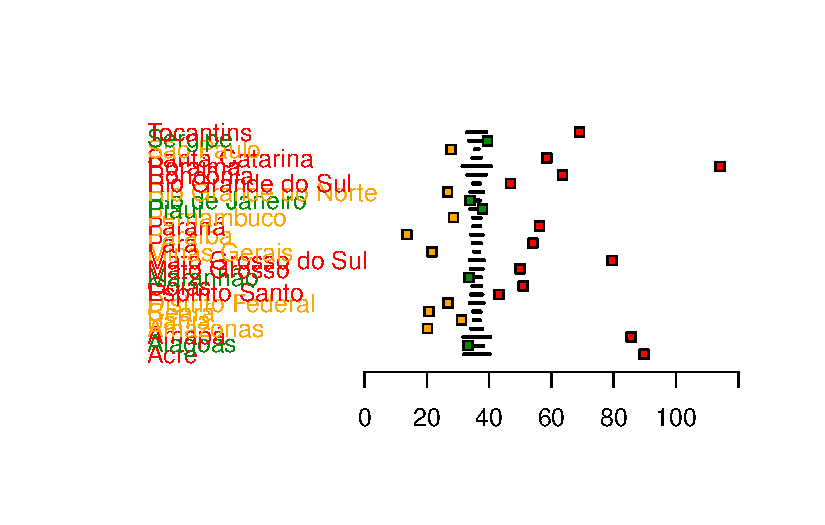
\includegraphics{intro_files/figure-pdf/unnamed-chunk-5-1.pdf}

\end{example}

\section{Inferência estatística}\label{inferuxeancia-estatuxedstica}

Denominamos por estatística qualquer função da amostra. Utilizamos
estatísticas para fazer as seguintes inferências:

\begin{itemize}
\item
  \emph{Estimação pontual}: trata-se de uma estatística com o objetivo
  de inferir o valor de \(\theta\). Tal estatística é denominada
  \textbf{estimador}.
\item
  \emph{Estimação por região}: trata-se de uma estatística, digamos
  \(T(\boldsymbol{X})\), com o objetivo de cobrir o valor de \(\theta\),
  ou seja, fazer a inferência \(\theta\in T(\boldsymbol{X})\). As
  estimações intervalares são as mais comuns, nas quais
  \(T(\boldsymbol{X})=(L(\boldsymbol{X}),U(\boldsymbol{X}))\).
\item
  \emph{Testes de hipóteses}: são estatísticas construídas para decidir
  se aceitamos a afirmação (hipótese) \(H:\theta\in \Theta_0\), onde
  \(\Theta_0\) é um subconjunto de \(\Theta\) conhecido por hipótese.
\end{itemize}

Note que a distribuição \textbf{a posteriori} é função da amostra.
Assim, toda função desta distribuição é uma estatística. Assim:

\begin{itemize}
\item
  \emph{Estimação pontual}: em geral é uma medida que representa a
  região de alta densidade (ou probabilidade) da \textbf{posteriori}. A
  média da posteriori, assim como a mediana ou a moda são escolhas
  comuns.
\item
  \emph{Estimação por regiões}: em geral procuramos por uma região \(T\)
  da posteriori que satisfaça
  \(P(\theta\in T(\boldsymbol{x})|\boldsymbol{x})=\gamma\), onde
  \(\gamma\) é denominado nível de credibilidade (não confundir com
  nível de confiança)
\item
  \emph{Testes de hipóteses}: em geral, aceitamos
  \(H:\theta\in\Theta_0\) se \(P(H|\boldsymbol{x})\) é elevada.
\end{itemize}

\begin{example}[]\protect\hypertarget{exm-}{}\label{exm-}

Para o nosso exemplo, obtivemos
\(\theta|\boldsymbol{x}\sim\hbox{Gama}(953.8,37.1)\). Então, uma
estimativa pontual para \(\theta\) é

\[E(\theta|\boldsymbol{x})=\frac{953,8}{37,1}=25,7\] registros de
suicídios mensais.

Podemos obter os quantis de 2,5\% e 97,5\% para construir um intervalo
com 95\% de credibilidade:

\begin{Shaded}
\begin{Highlighting}[]
\FunctionTok{qgamma}\NormalTok{( }\FunctionTok{c}\NormalTok{(.}\DecValTok{025}\NormalTok{,.}\DecValTok{975}\NormalTok{), }\FloatTok{953.8}\NormalTok{, }\FloatTok{37.1}\NormalTok{)}
\end{Highlighting}
\end{Shaded}

\begin{verbatim}
[1] 24.10301 27.36583
\end{verbatim}

logo, inferimos que \(\theta\in(24.1,27.36)\) com probabilidade 0,95.

Por último, recorde-se que discutimos, utilizando apenas os dados
nacionais, que \(\theta\) deveria está próximo de 22,8. Após observa a
amostra, existem evidências de que \(H:\theta>22,8\)? Para responder a
esse questionamento, podemos calcular

\[P(H|\boldsymbol{x})=P(\theta>22.8|\boldsymbol{x})\]

\begin{Shaded}
\begin{Highlighting}[]
\DecValTok{1}\SpecialCharTok{{-}}\FunctionTok{pgamma}\NormalTok{(}\FloatTok{22.8}\NormalTok{, }\FloatTok{953.8}\NormalTok{, }\FloatTok{37.1}\NormalTok{)}
\end{Highlighting}
\end{Shaded}

\begin{verbatim}
[1] 0.9998554
\end{verbatim}

logo, com uma probabilidade maior que 99,9\%, existem fortes evidências
de que o número médio mensal de suicídios no Amazonas é maior do que
22,8 registros por mês.

\end{example}

\section{Exercício}\label{exercuxedcio}

É fato que a taxa de suicídio é maior entre os homens, embora a
tentativa seja maior entre as mulheres. Uma das explicações está no fato
de que os homens tendem a utilizar métodos mais letais para o suicídio,
como armas de fogo, enquanto as mulheres são mais propensas a utilizar
métodos menos letais, como overdose de medicamentos.

Dados históricos, entre 1996 e 2017, sugerem que 79\% dos suicídios são
cometidos por homens.

Seja \(\rho\) a probabilidade de que um suicídio seja cometido por
alguém do sexo masculino no Estado do Amazonas. Considere a priori
\(\rho\sim\hbox{Beta}(a,b)\), onde sabemos que

\[f(\rho)\propto \rho^{a-1}(1-\rho)^{b-1},\] \[E(\rho)=\frac{a}{a+b},\]
e \[Var(\rho)=\frac{E(\rho)(1-E(\rho))}{a+b+1}.\]

\begin{itemize}
\item
  Encontre valores de \(a\) e \(b\) que reflitam a média de 0,79 mas que
  não restrinjam demais os valores possíveis para \(\rho\)
\item
  No Amazonas, entre os anos 2021 e 2023, dos 933 registros de
  suicídios, 726 foram cometidos por homens. Considere então o modelo
  \(X|\rho\sim\hbox{Binomial}(933,\rho)\). Mostre que
  \[f(\theta|x)\propto \rho^{726+a-1}(1-\rho)^{207+b-1}\] e conclua que
  \(\rho|x\sim\hbox{Beta}(a+933,b+207)\).
\item
  Estime \(\theta\) e construa um intervalo de 95\% de credibilidade
\item
  Teste a hipótese de que, para o Amazonas, a probabilidade de um
  indivíduo do sexo masculino cometer suicídio é maior do que 79\%.
\item
  Para problemas envolvendo proporções, é comum o uso a priori
  \(\rho\sim\hbox{Uniforme}(0,1)\), que é equivalente à
  \(\rho\sim\hbox{Beta}(1,1)\). Refaça este exercício com essa priori e
  discuta sobre as diferenças encontradas tanto nas estimações quanto no
  teste de hipóteses.
\end{itemize}

\section{Resumo da aula 1}\label{resumo-da-aula-1}

\begin{itemize}
\item
  Existem duas fontes de informação na inferência bayesiana: os dados
  (verossimilhança) e a informação anterior (priori)
\item
  A informação \textbf{a priori} é subjetiva: pessoas diferentes têm
  prioris diferentes
\item
  O Teorema de Bayes combina as duas fontes em uma nova informação, dada
  pela distribuição \textit{a posteriori}
\item
  Os objetivos da inferência (estimação e testes) são feitos a partir da
  distribuição \textbf{a posteriori}
\end{itemize}

\bookmarksetup{startatroot}

\chapter{Famílias conjugadas}\label{famuxedlias-conjugadas}

\section{Dados que serão utilizados neste
capítulo}\label{dados-que-seruxe3o-utilizados-neste-capuxedtulo}

\begin{Shaded}
\begin{Highlighting}[]
\FunctionTok{require}\NormalTok{(gsheet)}
\end{Highlighting}
\end{Shaded}

\begin{verbatim}
Carregando pacotes exigidos: gsheet
\end{verbatim}

\begin{verbatim}
Warning: pacote 'gsheet' foi compilado no R versão 4.4.3
\end{verbatim}

\begin{Shaded}
\begin{Highlighting}[]
\NormalTok{url }\OtherTok{\textless{}{-}} \StringTok{\textquotesingle{}https://docs.google.com/spreadsheets/d/1dLDCjA9a8UgXA9sJ1TNCVvRCDFITalewGkHlc\_\_Eg20/edit?usp=sharing\textquotesingle{}} 
\NormalTok{dt }\OtherTok{\textless{}{-}} \FunctionTok{gsheet2tbl}\NormalTok{(url)}
\FunctionTok{head}\NormalTok{(dt)}
\end{Highlighting}
\end{Shaded}

\begin{verbatim}
# A tibble: 6 x 5
  REGIAO              TIPO     SEXO  PERIODO   TOTAL
  <chr>               <chr>    <chr> <chr>     <dbl>
1 Região Norte        AGRESSAO Masc  2001-2003  7628
2 Região Nordeste     AGRESSAO Masc  2001-2003 29652
3 Região Sudeste      AGRESSAO Masc  2001-2003 63411
4 Região Sul          AGRESSAO Masc  2001-2003 12428
5 Região Centro-Oeste AGRESSAO Masc  2001-2003  9319
6 Região Norte        AGRESSAO Fem   2001-2003   677
\end{verbatim}

\section{Família de distribuições
conjugadas}\label{famuxedlia-de-distribuiuxe7uxf5es-conjugadas}

::: \{\#def-Priori conjugada\} Dizemos que a priori
\(f(\boldsymbol{\theta})\) é conjugada para a verossimilhança
\(L(\boldsymbol{\theta})\) se \emph{priori} e \emph{posteriori}
pertencem à mesma família de distribuições. :::

\begin{example}[]\protect\hypertarget{exm-}{}\label{exm-}

Sejam \(X_1,\ldots,X_n\) variáveis aleatórias independentes com
\(X|\theta\sim \hbox{Bernoulli}(\theta)\) e
\(\theta\sim\hbox{Beta}(a,b)\). Então

\[\begin{align}
    f(\theta|\boldsymbol{x})&\varpropto L(\theta)f(\theta) = \underbrace{\theta^{\sum_{i=1}^{n}x_i} (1-\theta)^{n-\sum_{i=1}^{n}x_i}}_{L(\theta)}\underbrace{\theta^{a-1}(1-\theta)^{b-1}}_{f(\theta)}\\
    &=\theta^{a+\sum_{i=1}^n x_i-1}(1-\theta)^{b+n-\sum_{i=1}^{n}x_i-1},
    \end{align}\] logo
\(\theta|\boldsymbol{x}\sim\hbox{Beta}(a+\sum_{i=1}^{n}x_i,b+n-\sum_{i=1}^{n}x_i)\)
e a \emph{priori} beta é conjugada para a verossimilhança Bernoulli.

\end{example}

Famílias conjugadas são extremamente úteis tanto sob o ponto de vista
algébrico quanto computacional. Entretanto, note que a definição de
família conjugada é ampla. Por exemplo, \emph{priori} e
\emph{posteriori} sempre pertencem à grande família de todas as
distribuições de probabilidade, sendo esta a família conjugada trivial.

Famílias conjugadas não triviais são raras, existindo principalmente
quando a distribuição condicional dos dados pertence à família
exponencial.

::: \{\#def-Família exponencial\} Definição Considere que \(\Theta\) tem
dimensão \(k\). Dizemos que \(X|\boldsymbol{\theta}\) pertence à família
exponencial (natural) se
\[f(x|\boldsymbol{\theta})=h(x)a(\boldsymbol{\theta})\exp\left\{\sum_{j=1}^k t_j(x)\theta_j\right\},\]
onde \(\mathcal{X}\) não depende de \(\boldsymbol{\theta}\). Além disso,
para a amostra (iid )\(X_1,\ldots,X_n|\boldsymbol{\theta}\),
\[f(\boldsymbol{x}|\boldsymbol{\theta})=h(\boldsymbol{x})a(\boldsymbol{\theta})^n\exp\left\{\sum_{j=1}^k T_j\theta_j\right\},\]
onde \(T_j=\sum_{i=1}^{n}t_j(x_i)\) :::

\begin{theorem}[]\protect\hypertarget{thm-}{}\label{thm-}

Se \(X|\boldsymbol{\theta}\) pertence à família exponencial, então
\[f(\boldsymbol{\theta})=c(\boldsymbol{r},s)a(\boldsymbol{\theta})^s\exp\left\{\sum_{j=1}^k r_j\theta_j\right\}\]
é uma \emph{priori} conjugada (ver O'Hagan (2005) para a existência
dessa distribuição). A \emph{posteriori} será dada por
\[f(\boldsymbol{\theta}|\boldsymbol{x})=c\left(\sum_{j=1}^k r_j+T_j,s+n\right)a(\boldsymbol{\theta})^{s+n}\exp\left\{\sum_{j=1}^k(r_j+T_j)\theta_j\right\}\]

\end{theorem}

Prova

\[\begin{align}
f(\boldsymbol{\theta}|\boldsymbol{x})&\varpropto \underbrace{a(\boldsymbol{\theta})^ne^{\sum_{j=1}^kT_j\theta_k}}_{L(\boldsymbol{\theta})}\underbrace{a(\boldsymbol{\theta})^s e^{\sum_{j=1}^k r_j\theta_k}}_{f(\boldsymbol{\theta})}\\
&a(\boldsymbol{\theta})^{n+s}e^{(\sum_{j=1}^{k}T_j+r_j)\theta_j}
\end{align}\]

Considere que \(\boldsymbol{\theta}\sim C(\boldsymbol{r},s)\) é a
distribuição conjugada da verossimilhança. Isto implica em
\(\boldsymbol{\theta}|\boldsymbol{x}\sim\hbox{C}(\boldsymbol{T}+\boldsymbol{r},s+n)\).
Note que a \emph{posteriori} atualiza a informação de \(s\) para \(s+n\)
e de \(r_j\) para \(T_j+r_j\). Logo, se imaginarmos que a priori é um
experimento hipotético, \(s\) seria o tamanho da amostra e
\(\boldsymbol{r}\) seriam as estatísticas suficientes deste modelo.

Abaixo, segue uma lista de algumas prioris conjugadas para modelos na
família exponencial.

\[\begin{array}{c|c|c}\hline
\text{Modelo} & \text{Priori} & \text{Posteriori} \\ \hline
\text{Bernoulli}(\theta) & \text{Beta}(a,b) & \text{Beta}(a+\sum_i x_i, b+n-\sum_i x_i) \\ \hline
\text{Poisson}(\lambda) & \text{Gama}(a,b) & \text{Gama}(a+\sum_i x_i, b+n) \\ \hline
\text{Multinomial}(p_1,\ldots,p_k) & \text{Dirichlet}(a_1,\ldots,a_k) & \text{Dirichlet}(a_1+x_1,\ldots,a_k+x_k) \\
\text{Exponencial}(\lambda) & \text{Gama}(a,b) & \text{Gama}(a+n, b+x_i) \\
\text{Normal}(\mu,\phi^{-1})&\text{Normal-Gama}(m_0,n_0,v_0,s_0^2)&
\text{Normal-Gama}(m_1,n_0+n,v_0+n,s_1^2)\\
& & m_1= \frac{n}{n_1}\bar{x}+\frac{n_0}{n_1}m_0\\
& & s_1^2=\frac{n_0n}{n_1^2}(\bar{x}-m_0)^2 + \frac{(n-1)s^2+n_0 s_0^2}{n_1} \\ \hline
\end{array}
\]

\section{Prioris conjugadas fora da família
exponencial}\label{prioris-conjugadas-fora-da-famuxedlia-exponencial}

Famílias conjugadas fora da família exponencial são raras. Seja
\(X_1,\ldots,X_n\) variáveis aleatória independentes com
\(X_1|\phi,\psi\sim\hbox{Binomial Negativa}(\psi,\phi)\), onde

\[f(x|\phi,\psi)=\frac{\Gamma(x+\psi)}{\Gamma(\psi)x!}\phi^\psi (1-\phi)^x,\]
com \(\psi>0\), \(\phi\in(0,1)\) e \(x\in\mathbb{N}\). Se \(\psi\) é
conhecido, então
\[L(\boldsymbol{\theta})=\underbrace{\left[\frac{\prod_{i=1}^n\Gamma(x_i+\psi)}{\Gamma(\psi)^n\prod_{i=1}^n x_i!}\right]}_{h(\boldsymbol{x})}\underbrace{\phi^{n\psi}}_{a(\phi)}\exp\left\{ \underbrace{\sum_{i=1}^n x_i}_{t(\boldsymbol{x})} \underbrace{\log(1-\phi)}_{w(\phi)}\right\} \]

Então, \[\begin{align}
f(\phi|\psi)&=c(r,s)a(\phi)^s e^{rw(\phi)}\\
&=c(r,s)\phi^{s\psi}(1-\phi)^{r}
\end{align}\] é uma \(*priori*\) conjugada. Da expressão acima segue que
\(\phi|\psi \sim \hbox{Beta}(s\psi+1,r+1)\). A \(*posteriori*\)
(condicional) por sua vez é dada por
\[f(\phi|\boldsymbol{x},\psi)\varpropto \phi^{\psi(s+n)}(1-\phi)^{r+\sum_{i=1}^{n}x_i},\]
onde ainda
\(\phi|\psi,\boldsymbol{x}\sim\hbox{Beta}(\psi(s+n)+1,r+\sum_{i=1}^{n}x_i+1)\)
Note que para fazer a inferência completa, ainda necessitamos de
\(\psi|\boldsymbol{x}\), uma vez que
\[f(\phi,\psi|\boldsymbol{x})=f(\phi|\psi,\boldsymbol{x})f(\psi|\boldsymbol{x}).\]
Outro método de obter a conjunta \((\phi,\psi|\boldsymbol{x})\), sem a
necessidade de calcular \(\psi|\boldsymbol{x}\) será discutido na
próxima aula.

\bookmarksetup{startatroot}

\chapter{O estimador de bayes}\label{o-estimador-de-bayes}

Considere o problema de tomar alguma decisão sobre \(\theta\) utilizando
uma estatística \(T(\mathbf{x})\).

Podemos determinar o quão ruim é a nossa decisão definindo uma função de
perda \(\mathcal{L}(\theta,T)\), com as seguintes características:

\begin{itemize}
\item
  \(\mathcal{L}(\theta,T)=0\) sempre que \(T\) for a decisão correta em
  relação à \(\theta\)
\item
  \(\mathcal{L}(\theta,T)>0\) em caso contrário.
\end{itemize}

Por exemplo, se \(T\) for um estimador para \(\theta\), a decisão
correta seria ter \(T=\theta\). Além disso, quanto mais afastado \(T\)
estiver de \(\theta\), pior é a decisão e maior deveria ser a perda.

No problema de estimação pontual, é usual utilizar a perda quadrática:
\[\mathcal{L}(\theta,T)=(T-\theta)^2,\] cujo esboço do gráfico é dado
abaixo:

\begin{Shaded}
\begin{Highlighting}[]
\FunctionTok{plot.new}\NormalTok{()}
\FunctionTok{plot.window}\NormalTok{(}\AttributeTok{xlim=}\FunctionTok{c}\NormalTok{(}\SpecialCharTok{{-}}\DecValTok{2}\NormalTok{,}\DecValTok{2}\NormalTok{), }\AttributeTok{ylim=}\FunctionTok{c}\NormalTok{(}\DecValTok{0}\NormalTok{,}\DecValTok{4}\NormalTok{))}
\FunctionTok{curve}\NormalTok{( x}\SpecialCharTok{\^{}}\DecValTok{2}\NormalTok{,}\SpecialCharTok{{-}}\DecValTok{2}\NormalTok{,}\DecValTok{2}\NormalTok{, }\AttributeTok{lwd =} \DecValTok{2}\NormalTok{, }\AttributeTok{add =}\NormalTok{ T)}
\FunctionTok{axis}\NormalTok{(}\DecValTok{1}\NormalTok{, }\AttributeTok{at =} \FunctionTok{c}\NormalTok{(}\SpecialCharTok{{-}}\DecValTok{2}\NormalTok{,}\SpecialCharTok{{-}}\DecValTok{1}\NormalTok{,}\DecValTok{0}\NormalTok{,}\DecValTok{1}\NormalTok{,}\DecValTok{2}\NormalTok{), }\AttributeTok{labels =} \FunctionTok{c}\NormalTok{(}\FunctionTok{expression}\NormalTok{(theta }\SpecialCharTok{{-}}\DecValTok{2}\NormalTok{),}\FunctionTok{expression}\NormalTok{(theta }\SpecialCharTok{{-}}\DecValTok{1}\NormalTok{),}\FunctionTok{expression}\NormalTok{(theta),}\FunctionTok{expression}\NormalTok{(theta }\SpecialCharTok{+}\DecValTok{1}\NormalTok{),}\FunctionTok{expression}\NormalTok{(theta }\SpecialCharTok{+}\DecValTok{2}\NormalTok{) ))}
\FunctionTok{axis}\NormalTok{(}\DecValTok{2}\NormalTok{)}
\FunctionTok{title}\NormalTok{( }\AttributeTok{ylab =} \StringTok{\textquotesingle{}Perda quadrática\textquotesingle{}}\NormalTok{,}\AttributeTok{xlab =} \StringTok{\textquotesingle{}T\textquotesingle{}}\NormalTok{)}
\end{Highlighting}
\end{Shaded}

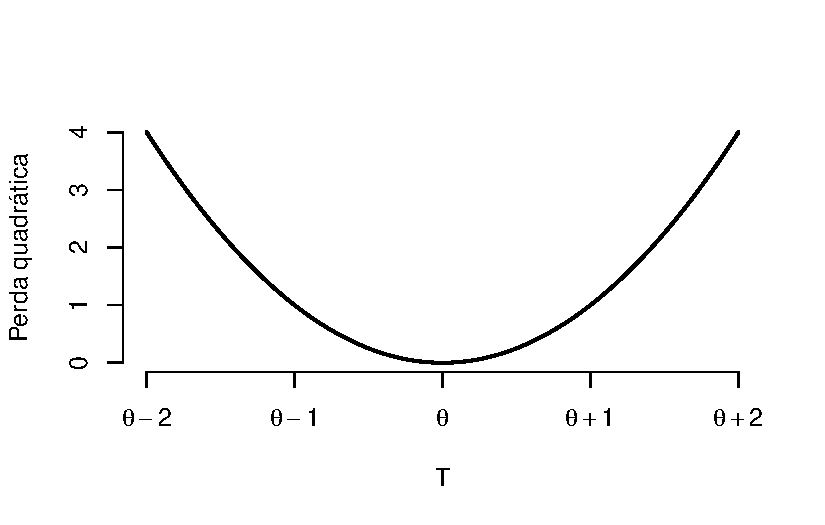
\includegraphics{estimacao_files/figure-pdf/unnamed-chunk-1-1.pdf}

Para uma decisão \(T\) podemos calcular a perda média
\[R_T(\theta)=E(\mathcal{L}(\theta,T))=\int L(\theta,T(\mathbf{x}))f(\mathbf{x}|\theta)d\mathbf{x}\]
A função acima é conhecida como risco da decisão \(T\) e é variável em
\(\theta\). Seu uso é simples: se \(R_T(\theta)<R_U(\theta)\), então em
média a decisão \(T\) tem menor perda que \(U\). Assim, a melhor escolha
entre as duas decisão é \(U\).

O risco associado à perda quadrática é denominado erro quadrático médio:

\[R_T(\theta)=E(T-\theta)^2= Var(T)+(E(T|\theta)-\theta)^2\] Ele possui
papel importante na inferência pontual frequentista, como por exemplo,
para definir o melhor estimador não viciado de variância uniformemente
mínima.

O risco de Bayes da decisão \(T\) é o valor esperado do seu respectivo
risco \textit{a priori}, \[r_T=\int R_T(\theta)f(\theta)d\theta,\] sendo
portanto uma constante. Qualquer decisão com o menor risco para todo
\(\theta\) também tem o menor risco de Bayes. Dizemos que \(T\) é o
estimador de Bayes se \(r_T<r_U\) para qualquer decisão \(U\).

Teorema

O estimador \(T\) que minimiza
\[\int \mathcal{L}(\theta,T(\mathbf{x}))f(\theta|\mathbf{x})d\theta\] é
o estimador de Bayes.

Exemplo

Vamos encontrar o estimador de Bayes para a perda quadrática. Temos que

\[\begin{align*}\int \mathcal{L}(\theta,T(\mathbf{x}))f(\theta|\mathbf{x})d\theta&=\int (T(\mathbf{x})-\theta)^2f(\theta|\mathbf{x})d\theta\\
    &=T(\mathbf{x})^2 +\int \theta^2f(\theta|\mathbf{x})d\theta-2T(\mathbf{x})\int \theta f(\theta|\mathbf{x})d\theta\\
    &= T(\mathbf{x})^2 + E(\theta^2|\mathbf{x}) -2T(\mathbf{x})E(\theta|\mathbf{x})\\
    &= T(\mathbf{x})^2 + E(\theta^2|\mathbf{x}) -2T(\mathbf{x})E(\theta|\mathbf{x}) \pm E(\theta|\mathbf{x})^2\\
    &=\left( T(\mathbf{x}) - E(\theta|\mathbf{x})\right)^2 +E(\theta^2|\mathbf{x})-E(\theta|\mathbf{x})^2\\
    &=\left( T(\mathbf{x}) - E(\theta|\mathbf{x})\right)^2 +Var(\theta|\mathbf{x})
\end{align*}\] A função acima é minimizada em
\(T(\mathbf{x})=E(\theta|\mathbf{x})\). Disto, mostra-se que
\[r_T\geq Var(\theta|\mathbf{x})\] e a variância da posteriori pode ser
utilizada como medida de erro. Como a unidade deste erro está ao
quadrado, é usual utilizarmos o desvio padrão da posteriori como medida
de erro.

\begin{example}[]\protect\hypertarget{exm-}{}\label{exm-}

Seja \(X_1,\ldots,X_n\) uma amostra aleatória do modelo
Exponencial(\(\theta\)) e considere a priori
\(\theta\sim\hbox{Gama}(a,b)\). Sabemos que
\(\theta|\boldsymbol{x}\sim\hbox{Gama}(s+n,r+\sum_{i=1}^n x_i)\). Então,
o estimador de Bayes segundo a perda quadrática é
\[T(\boldsymbol{x})=E(\theta|\boldsymbol{x})=\frac{s+n}{r+\sum_{i=1}^n x_i},\]
e o erro associado é
\[\sqrt{Var(\theta|\boldsymbol{x})}=\sqrt{\frac{s+n}{(r+\sum_{i=1}^n x_i)^2}}=\sqrt{\frac{E(\theta|\boldsymbol{x})^2}{s+n}}=\frac{E(\theta|\boldsymbol{x})}{\sqrt{n+s}}.\]

Note que, como esperado, o erro decresce na medida que \(n\) cresce.

\end{example}

\bookmarksetup{startatroot}

\chapter{O modelo Bernoulli}\label{o-modelo-bernoulli}

\section{O modelo univariado}\label{o-modelo-univariado}

A distribuição \(F\) é dita pertencer à família Bernoulli, com parâmetro
\(\theta\in(0,1)\) se sua função de probabilidade é dada por
\[f(x|\theta)=\theta^x(1-\theta)^{1-x},\] com \(x\in\{0,1\}\). É
imediato que \(\theta\) representa a probabilidade de \(\{X=1\}\), sendo
este evento conhecido como `sucesso' em alguns textos (em contrapartida,
\(\{X=0\}\) é conhecido como `fracasso').

Esta distribuição faz a importante conexão entre variáveis categóricas e
aleatórias, tendo papel fundamental na inferência não paramétrica. Por
exemplo, seja \(S\) o sexo de um indivíduo selecionado ao acaso. Tal
variável é categórica, podendo assumir os resultados \(A=\)\{feminino\}
ou \(A^c\). Contudo, pode-se definir a variável \(X=I(A)\), onde
\(I(.)\) é a função indicadora, definida por
\[I(A)=\left\{\begin{array}{ll} 1,&\hbox{ se $A$ ocorre,} \\ 0,&\hbox{ se $A^c$ ocorre.}\end{array}\right.
\] Deste modo \(X\sim\hbox{Bernoulli}(\theta)\).

Como discutido anteriormente, o modelo Bernoulli(\(\theta\)) pertence à
família exponencial e sua distribuição conjugada é a Beta\((a,b)\). A
distribuição a posteriori é dada por

\[f(\theta|\boldsymbol{x})\propto \theta^{a+\sum_{i=1}^n x_i-1}(1-\theta)^{n-\sum_{i=1}^n x_i+b-1},\]
ou seja,
\(\theta|\boldsymbol{x}\sim\hbox{Beta}(a+\sum_{i=1}^n x_i,n-\sum_{i=1}^n x_i + b).\)
Observe que \(a\) pode ser interpretado como o número de sucessos a
priori e \(b\) o número de fracassos. É comum utilizarmos a priori
Beta\((1,1)\), que é equivalente à Uniforme(0,1), como priori pouco
informativa.

\begin{example}[]\protect\hypertarget{exm-}{}\label{exm-}

Um estudo investiga a eficácia de uma nova campanha de vacinação contra
a gripe em uma grande cidade. Antes da campanha, a taxa de vacinação na
população adulta era de 40\%. Após a campanha, uma amostra aleatória de
500 adultos revelou que 250 deles foram vacinados. Os pesquisadores
querem determinar se a campanha aumentou significativamente a taxa de
vacinação.

Seja \(\theta\) a nova taxa de vacinação. Estamos interessados em testar
a hipótese de que \(\theta>0,4\). Considerando que o evento de interesse
é um adulto vacinado, teremos que \(x_i=1\) se o \(i\)-ésimo adulto da
amostra foi vacinado e \(x_i=0\) em caso contrário. Utilizando a priori
Beta(1,1), teremos
\(\theta|x_1,\ldots,x_{500}\sim\hbox{Beta}(251,251)\). Deste modo a
probabilidade a posteriori da hipótese é

\[P(\theta>0,4|\boldsymbol{x})=\int_{0,4}^1 f(\theta|\boldsymbol{x})d\theta.\]
Utilizando o \texttt{R}, obtemos

\begin{Shaded}
\begin{Highlighting}[]
\DecValTok{1}\SpecialCharTok{{-}}\FunctionTok{pbeta}\NormalTok{(.}\DecValTok{4}\NormalTok{,}\DecValTok{251}\NormalTok{,}\DecValTok{251}\NormalTok{)}
\end{Highlighting}
\end{Shaded}

\begin{verbatim}
[1] 0.999997
\end{verbatim}

logo, a probabilidade de que a campanha aumentou a taxa de vacinação é
maior que 99,999\%.

\end{example}

\begin{example}[]\protect\hypertarget{exm-}{}\label{exm-}

\textbf{As duas clínicas}

Em 1846, Ignaz Philipp Semmelweis se tornou assistente na Primeira
Clínica de Obstetrícia do Hospital Geral de Viena, Áustria (algo como o
residente chefe). Neste hospital o parto era oferecido de gratuitamente,
pois o mesmo serveria de treinamento para os médicos e parteiras.

Naquela época, a febre puerperal era comum e muitas vezes fatal, sendo
que a mortalidade variava entre 10\% a 35\%.

Haviam duas maternidades no Hospital Geral de Viena, conhecidas como a
Primeira e a Segunda. A Primeira era considerada um local de morte e era
evitada quando possível. Abaixo temos os dados registrados pelo
Dr.~Semmelweis

\[\begin{array}{c|cc|cc}\hline \hbox{} & \hbox{Primeira} & \hbox{Clínica} & \hbox{Segunda} & \hbox{Clínica}\\ \hline
\hbox{Ano} & \hbox{Partos} & \hbox{Mortes} &\hbox{Partos} & \hbox{Mortes} \\ \hline 
1841 & 3036 & 237 & 2442 & 86 \\
1842 & 3287 & 518 & 2659 & 202 \\
1843 & 3060 & 274 & 2739 & 164 \\
1844 & 3157 & 260 & 2956 & 68 \\
1845 & 3492 & 241 & 3241 & 66 \\
1846 & 4010 & 459 & 3754 & 105 \\ \hline
\hbox{Total} & 20.042 & 1.989 & 17.791 & 691 \\ \hline
\end{array}\]

Pode-se considerar que cada parto gera duas possibilidades de eventos: a
sobrivência ou a morte da mãe. Considere que, dentro da mesma clínica,
esses eventos para cada mãe são indepentes e possuem a mesma
probabilidade. Seja \(\alpha\) a probabilidade de morte na Primeira
Clínica e \(\beta\) a mesma probabilidade para a Segunda Clínica. Então,
as funções de verossimilhança para cada probabilidade são

\[\begin{align}L(\alpha)&\propto \alpha^{1989} (1-\alpha)^{18053}\\L(\beta)&\propto \beta^{691} (1-\beta)^{17100}\end{align}\]
Utilizando distribuição Uniforme(0,1) como priori para \(\alpha\) e
\(\beta\), teremos que

\[\begin{align}\alpha|\boldsymbol{x}&\sim \hbox{Beta}(1990,18054) \\\beta|\boldsymbol{x}&\sim \hbox{Beta}(692,17101)\end{align}\]

Abaixo, mostramos as duas posterioris, de onde podemos concluir que a
probabilidade de morte na Primeira Clínica é certamente maior que na
Segunda.

\begin{Shaded}
\begin{Highlighting}[]
\FunctionTok{curve}\NormalTok{(}\FunctionTok{dbeta}\NormalTok{(x,}\DecValTok{1990}\NormalTok{,}\DecValTok{18054}\NormalTok{),}\FloatTok{0.03}\NormalTok{,.}\DecValTok{11}\NormalTok{, }\AttributeTok{lwd =} \DecValTok{2}\NormalTok{,}\AttributeTok{ylab=}\StringTok{\textquotesingle{}Densidades a posteriori\textquotesingle{}}\NormalTok{,}\AttributeTok{xlab=}\StringTok{\textquotesingle{}Probabilidade de morte\textquotesingle{}}\NormalTok{,}\AttributeTok{ylim=}\FunctionTok{c}\NormalTok{(}\DecValTok{0}\NormalTok{,}\DecValTok{300}\NormalTok{))}
\FunctionTok{curve}\NormalTok{(}\FunctionTok{dbeta}\NormalTok{(x,}\DecValTok{692}\NormalTok{,}\DecValTok{17101}\NormalTok{), }\AttributeTok{lwd =} \DecValTok{2}\NormalTok{, }\AttributeTok{add =}\NormalTok{ T)}
\FunctionTok{text}\NormalTok{(}\FunctionTok{c}\NormalTok{(.}\DecValTok{04}\NormalTok{,.}\DecValTok{1}\NormalTok{),}\FunctionTok{c}\NormalTok{(}\DecValTok{290}\NormalTok{,}\DecValTok{210}\NormalTok{),}\FunctionTok{c}\NormalTok{(}\StringTok{\textquotesingle{}Segunda Clínica\textquotesingle{}}\NormalTok{,}\StringTok{\textquotesingle{}Primeira Clínica\textquotesingle{}}\NormalTok{))}
\end{Highlighting}
\end{Shaded}

\includegraphics{bernoulli_files/figure-pdf/unnamed-chunk-2-1.pdf}

O Dr.~Semmelweis ainda não tinha descoberto o motivo dessas mortes até a
morte de seu amigo Jakob Kolletschka, que se cortou acidentalmente com
um bisturi durante uma autópsia. Durante a autópsia de Jakob, o
Dr.~Semmelweis viu semelhanças com as autópsias as mulheres que havia
morrido por febre puerperal.

Na Primeira Clínica estudavam os alunos de medicina, que realizavam
autópsias. Na Segunda Clínica estudavam as parteiras, que não realizam
autópsias. A sua hipótese foi: estudantes de medicina carregavam
partículas cadavéricas que causavam a febre puerperal. Com essa
hipótese, ele instituiu que todos os médicos deveriam lavar as mãos
antes dos partos em maio de 1847. Abaixo, seguem os dados de Junho de
1848 até Março 1849, apenas para a Primeira Clínica

\[\begin{array}{c|cc} \hline \hbox{Período} & \hbox{Partos} & \hbox{Mortes}\\ \hline
\hbox{Jun/1847-Dez/1847} & 1841 & 56 \\ 
\hbox{Jan/1848-Dez/1848} & 3556 & 45 \\ 
\hbox{Jan/1849-Mar/1849} & 1198 & 41 \\ \hline
\hbox{Total} & 6.595 & 142 \\ \hline
\end{array}\]

Seja \(\gamma\) a probabilidade de morte por febre puerperal na Primeira
Clínica após a instrução de lavagem das mãos. Sua função de
verossimilhança é

\[L(\gamma)\propto \gamma^{142}(1-\gamma)^{6453}.\] Assumindo a priori
Uniforme(0,1) para \(\gamma,\) teremos que
\(\gamma|\boldsymbol{x}\sim\hbox{Beta}(143,6454)\). Abaixo, apresentamos
o gráfico das três densidades a posteriori obtidas, mostrando que
\(\gamma\) é certamente menor que as outras probabilidades.

\begin{Shaded}
\begin{Highlighting}[]
\FunctionTok{curve}\NormalTok{(}\FunctionTok{dbeta}\NormalTok{(x,}\DecValTok{1990}\NormalTok{,}\DecValTok{18054}\NormalTok{),}\DecValTok{0}\NormalTok{,.}\DecValTok{11}\NormalTok{, }\AttributeTok{lwd =} \DecValTok{2}\NormalTok{,}\AttributeTok{ylab=}\StringTok{\textquotesingle{}Densidades a posteriori\textquotesingle{}}\NormalTok{,}\AttributeTok{xlab=}\StringTok{\textquotesingle{}Probabilidade de morte\textquotesingle{}}\NormalTok{,}\AttributeTok{ylim=}\FunctionTok{c}\NormalTok{(}\DecValTok{0}\NormalTok{,}\DecValTok{300}\NormalTok{))}
\FunctionTok{curve}\NormalTok{(}\FunctionTok{dbeta}\NormalTok{(x,}\DecValTok{692}\NormalTok{,}\DecValTok{17101}\NormalTok{), }\AttributeTok{lwd =} \DecValTok{2}\NormalTok{, }\AttributeTok{add =}\NormalTok{ T)}
\FunctionTok{curve}\NormalTok{(}\FunctionTok{dbeta}\NormalTok{(x,}\DecValTok{143}\NormalTok{,}\DecValTok{6454}\NormalTok{), }\AttributeTok{lwd =} \DecValTok{2}\NormalTok{, }\AttributeTok{add =}\NormalTok{ T)}

\FunctionTok{text}\NormalTok{(}\FunctionTok{c}\NormalTok{(.}\DecValTok{01}\NormalTok{,.}\DecValTok{04}\NormalTok{,.}\DecValTok{1}\NormalTok{),}\FunctionTok{c}\NormalTok{(}\DecValTok{250}\NormalTok{,}\DecValTok{290}\NormalTok{,}\DecValTok{212}\NormalTok{),}\FunctionTok{c}\NormalTok{(}\StringTok{\textquotesingle{}Primeira Clínica }\SpecialCharTok{\textbackslash{}n}\StringTok{(1847{-}1849)\textquotesingle{}}\NormalTok{,}\StringTok{\textquotesingle{}Segunda Clínica\textquotesingle{}}\NormalTok{,}\StringTok{\textquotesingle{}Primeira Clínica}\SpecialCharTok{\textbackslash{}n}\StringTok{(1841{-}1846)\textquotesingle{}}\NormalTok{))}
\end{Highlighting}
\end{Shaded}

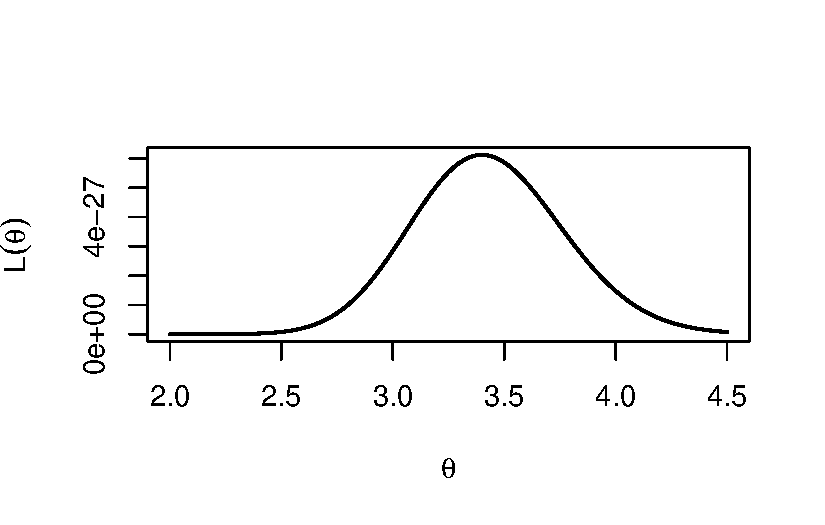
\includegraphics{bernoulli_files/figure-pdf/unnamed-chunk-3-1.pdf}

Após a publicação de seus achados, as ideia do Dr.~Semmelweis foram
amplamente rejeitadas por seus colegas médicos, que se sentiram
ofendidos com a sugestão de que poderiam estar causando a morte de seus
pacientes. A rejeição e o ridículo que Semmelweis enfrentou levaram a um
declínio em sua saúde mental. Ele foi internado no hospício em 1865,
onde morreu pouco tempo depois. Morreu em 13 de agosto de 1865, em um
hospício em Viena, aos 47 anos. A causa exata de sua morte ainda é
debatida, mas a teoria mais aceita é que ele morreu de septicemia, uma
infecção sanguínea, após ser espancado pelos guardas do hospício.
\[\blacksquare\]

\end{example}

No exemplo anterior foi possível verificar graficamente que as
probabilidades de morte por febre puerperal em ambas as clínicas eram
distintas. Recordando que as respectivas probabilidades foram
identificadas por \(\alpha\) e \(\beta\), era evidente que
\(P(\alpha>\beta|\hbox{dados})=1\).

Quando a evidência gráfica não é clara, é necessário calcular tal
probabilidade. Sejam \(X_1,\ldots,X_n\) e \(Y_1,\ldots,Y_m\) duas
amostras aleatórias independentes com
\(X_i|\alpha\sim\hbox{Bernoulli}(\alpha)\) e
\(Y_i|\beta\sim\hbox{Bernoulli}(\beta)\). Considerando prioris
conjugadas, teremos que \(\alpha|\boldsymbol{x}\) e
\(\beta|\boldsymbol{y}\) possuem distribuição beta e são independentes.
Para testar uma hipótese do tipo \(H: \alpha>\beta\) é necessário
calcular

\[p=P(\alpha>\beta|\boldsymbol{x},\boldsymbol{y}).\] Contudo, podemos
definir a variável
\(A=\left\{\begin{array}{ll}1,&\alpha>\beta\\ 0,&\alpha\leq \beta\end{array}\right.\)
Deste modo, \(A\sim\hbox{Bernoulli}(p)\). Acontece que \(p=E(A)\) e,
pela Lei Forte dos Grandes Números, para a sequência \(A_1,A_2,\ldots,\)
teremos que
\[\frac{1}{B}\sum_{j=1}^B A_j\rightarrow E(A)=p,\;\; B\rightarrow\infty\]
Deste modo, se tivermos uma observação da amostra aleatória
\(A_1,\ldots,A_B\) é possível calcular \(p\) com boa precisão para \(B\)
suficientemente grande. Podemos obter essa amostra via simulação. Esse é
o princípio do Método de Monte Carlo.

\textbf{Método de Monte Carlo} Considere o problema de calcular
\[p=E(X).\] * Passo 1. Simule \(x_1,\ldots,x_B\) com \(B\)
suficientemente grande

\begin{itemize}
\tightlist
\item
  Passo 2. Estime \(p\) através de
\end{itemize}

\[\frac{1}{B}\sum_{j=1}^B x_j\]

Para calcular \(p=P(\alpha>\beta|\hbox{dados})\) apresentado
anteriormente, podemos realizar os seguintes passos:

\begin{itemize}
\item
  Passo 1. Escolha \(B\) suficientemente grande
\item
  Passo 2. Simule \(\alpha_1,\ldots,\alpha_B\) a posteriori
  \(\alpha|\hbox{x}\)
\item
  Passo 3. Simule \(\beta_1,\ldots,\beta_B\) a posteriori
  \(\beta|\hbox{y}\)
\item
  Passo 4. Calcule
\end{itemize}

\[\frac{1}{B}\sum_{j=1}^B I(\alpha_j>\beta_j)\]

\begin{example}[]\protect\hypertarget{exm-}{}\label{exm-}

\textbf{Naufrágio do Lusitania (1915)}

Em 7 de maio de 1915, durante a Primeira Guerra Mundial, o RMS
Lusitania, um luxuoso transatlântico britânico, navegava a cerca de 18
km da costa sul da Irlanda. A bordo, passageiros de diversas
nacionalidades, incluindo muitos americanos, desfrutavam de uma viagem
que deveria levá-los de Nova York a Liverpool. No entanto, o que era
para ser uma travessia rotineira transformou-se em tragédia quando o
navio foi torpedeado pelo submarino alemão U-20.

Atingido no lado estibordo, o Lusitania sofreu uma segunda explosão
interna, cuja causa ainda é debatida, e afundou em apenas 18 minutos. A
rapidez com que o navio submergiu, aliada à dificuldade de lançar os
botes salva-vidas, resultou na morte de 1.198 pessoas, entre passageiros
e tripulantes. O naufrágio do Lusitania gerou indignação internacional e
intensificou a pressão para que os Estados Unidos entrassem na guerra, o
que ocorreu dois anos depois.

O número de passageiros que morreram e sobreviveram em cada classe é
dado abaixo.

\[\begin{array}{l|cc} \hline
\hbox{Classe} & \hbox{Sobreviventes} & \hbox{Mortos} \\ \hline
\hbox{Primeira} & 113 & 177 \\
\hbox{Segunda} & 229 & 372 \\ 
\hbox{Terceira}  & 134 & 239 \\ \hline
\end{array}\]

Neste exemplo, vamos testar a hipótese de que tripulantes da Classe 1
tinham maior probabilidade de sobrevivência que os dados classes
inferiores. Seja \(\alpha,\beta,\gamma\) as probabilidades de
sobrevivência das classes 1, 2 e 3, respectivamente, Considerando uma
priori Beta(1,1) para cada classe, teremos que a posteriori para a
probabilidade de sobrevivência é dada por

\begin{itemize}
\tightlist
\item
  \(\alpha\sim\)Beta(114,178) para a classe 1
\item
  \(\beta\sim\)Beta(230,373) para a classe 2
\item
  \(\gamma\sim\)Beta(135,240) para a classe 3
\end{itemize}

O gráfico das posterioris é dado abaixo

\begin{Shaded}
\begin{Highlighting}[]
\FunctionTok{curve}\NormalTok{(}\FunctionTok{dbeta}\NormalTok{(x, }\DecValTok{114}\NormalTok{,}\DecValTok{178}\NormalTok{), }\AttributeTok{lwd =} \DecValTok{2}\NormalTok{, }\AttributeTok{ylim=}\FunctionTok{c}\NormalTok{(}\DecValTok{0}\NormalTok{,}\DecValTok{20}\NormalTok{), }\AttributeTok{ylab =} \StringTok{\textquotesingle{}Densidades das posterioris\textquotesingle{}}\NormalTok{, }\AttributeTok{xlab =} \StringTok{\textquotesingle{}Probabilidade de sobrevivência\textquotesingle{}}\NormalTok{, }\AttributeTok{xlim=}\FunctionTok{c}\NormalTok{(.}\DecValTok{2}\NormalTok{,.}\DecValTok{6}\NormalTok{))}
\FunctionTok{curve}\NormalTok{(}\FunctionTok{dbeta}\NormalTok{(x, }\DecValTok{230}\NormalTok{,}\DecValTok{373}\NormalTok{), }\AttributeTok{add =}\NormalTok{ T, }\AttributeTok{col =}\DecValTok{2}\NormalTok{, }\AttributeTok{lwd =} \DecValTok{2}\NormalTok{)}
\FunctionTok{curve}\NormalTok{(}\FunctionTok{dbeta}\NormalTok{(x, }\DecValTok{135}\NormalTok{,}\DecValTok{240}\NormalTok{), }\AttributeTok{add =}\NormalTok{ T ,}\AttributeTok{col =}\DecValTok{3}\NormalTok{, }\AttributeTok{lwd =} \DecValTok{2}\NormalTok{)}
\FunctionTok{legend}\NormalTok{(}\StringTok{\textquotesingle{}topright\textquotesingle{}}\NormalTok{,}\FunctionTok{c}\NormalTok{(}\StringTok{\textquotesingle{}Classe 1\textquotesingle{}}\NormalTok{,}\StringTok{\textquotesingle{}Classe 2\textquotesingle{}}\NormalTok{,}\StringTok{\textquotesingle{}Classe 3\textquotesingle{}}\NormalTok{), }\AttributeTok{lwd =}\DecValTok{2}\NormalTok{, }\AttributeTok{col=}\DecValTok{1}\SpecialCharTok{:}\DecValTok{3}\NormalTok{, }\AttributeTok{bty=}\StringTok{\textquotesingle{}n\textquotesingle{}}\NormalTok{)}
\end{Highlighting}
\end{Shaded}

\includegraphics{bernoulli_files/figure-pdf/unnamed-chunk-4-1.pdf}

Vamos simular uma amostra de tamanho \(B=1000000\) das posterioris de
\(\alpha,\beta,\gamma\).

\begin{Shaded}
\begin{Highlighting}[]
\NormalTok{B }\OtherTok{\textless{}{-}} \DecValTok{1000000}
\NormalTok{alfa }\OtherTok{\textless{}{-}} \FunctionTok{rbeta}\NormalTok{(B, }\DecValTok{114}\NormalTok{,}\DecValTok{178}\NormalTok{)}
\NormalTok{beta  }\OtherTok{\textless{}{-}} \FunctionTok{rbeta}\NormalTok{(B, }\DecValTok{230}\NormalTok{,}\DecValTok{373}\NormalTok{)}
\NormalTok{gama  }\OtherTok{\textless{}{-}} \FunctionTok{rbeta}\NormalTok{(B, }\DecValTok{135}\NormalTok{,}\DecValTok{240}\NormalTok{)}
\end{Highlighting}
\end{Shaded}

Vamos testar a hipótese de que a probabilidade de sobrevivência de um
indivíduo da Classe 1 foi maior que a de um indivíduo da Classe 2 e 3.

\begin{Shaded}
\begin{Highlighting}[]
\FunctionTok{set.seed}\NormalTok{(}\DecValTok{123}\NormalTok{)}
\FunctionTok{mean}\NormalTok{(alfa}\SpecialCharTok{\textgreater{}}\NormalTok{beta)}
\end{Highlighting}
\end{Shaded}

\begin{verbatim}
[1] 0.600988
\end{verbatim}

\begin{Shaded}
\begin{Highlighting}[]
\FunctionTok{mean}\NormalTok{(alfa}\SpecialCharTok{\textgreater{}}\NormalTok{gama)}
\end{Highlighting}
\end{Shaded}

\begin{verbatim}
[1] 0.789448
\end{verbatim}

Observe que \(P(\alpha>\gamma|\hbox{dados})\approx 0,78\), o que não dá
suporte para afirmar que a probabilidade de sobrevivência dos
tripulantes da primeira classe foi maior do que o da terceira.
\[\blacksquare\]

\end{example}

\section{O modelo multivariado}\label{o-modelo-multivariado}

A distribuição Bernoulli pode ser generalizada para o caso multivariado:
considere um evento aleatório com possibilidades \(A_1,\ldots,A_k\).
Seja \(X_j=I(A_j)\) e seja \(\theta_j\) a probabilidade do evento
resultar em \(A_j\). Então, o vetor \(\boldsymbol{X}=(X_1,\ldots,X_k)\)
tem distribuição Bernoulli multivariada, cuja função de probabilidade é
dada por
\[f(\boldsymbol{x}|\boldsymbol{\theta})=\prod_{j=1}^k\theta_j^{x_{j}},\]
onde \(x_j\in\{0,1\}\), \(\sum_{j=1}^kx_j=1\), \(\theta_j\in(0,1)\) e
\(\sum_{j=1}^k\theta_j=1\). É importante notar que vetor
\(\boldsymbol{\theta}\) tem apenas \(k-1\) parâmetros de fato, uma vez
que \(\theta_k=1-\sum_{j=1}^{k-1}\theta_j\). Conjuntos do tipo
\[\mathcal{S}^k=\left\{(\theta_1,\ldots,\theta_{k-1}):0<\theta_j<1,0<\sum_{j=1}^{k-1}\theta_j<1\right\}\]
são denominados simplex.

Seja \(\boldsymbol{x}_1,\ldots,\boldsymbol{x}_n\) uma amostra de vetores
Bernoulli Multivariada(\(\theta_1,\ldots,\theta_k\)), onde
\(\boldsymbol{x}_i=\{x_{i,1},\ldots,x_{i,k}\}\). Então,

\[\begin{align}L(\boldsymbol{\theta})&=\prod_{i=1}^nf(\boldsymbol{x}_i|\boldsymbol{\theta})=\prod_{i=1}^n\left(\prod_{j=1}^k \theta_j^{x_{i,j}}\right)=\prod_{j=1}^k \prod_{i=1}^n\theta_j^{x_{i,j}}\\&=\prod_{j=1}^k \theta_j^{\sum_{i=1}^nx_{i,j}}=\prod_{j=1}^n\theta_j^{n_j}\end{align}\]
onde \(n_j\) é o número de vezes que ocorreu a categoria \(A_j\). É
imediado que

\[L(\boldsymbol{\theta})=\exp\left\{\sum_{j=1}^k n_j\log(\theta_j)\right\},\]
o que implica que este modelo pertence à família exponencial. Seu modelo
conjugado é a Dirichlet(\(a_1,\ldots,a_k\)), cuja função densidade é
\[f(\theta_1,\ldots,\theta_k)=\frac{\Gamma\left(\sum_{j=1}^k a_j\right)}{\prod_{j=1}^k \Gamma(a_j)}\prod_{j=1}^k \theta^{a_j-1},\]
onde \((\theta_1,\ldots,\theta_{k-1})\) pertence ao simplex
\(\mathcal{S}^k\).

A Dirichlet\((a_1,\ldots,a_k)\) possui as seguintes propriedades:

\begin{itemize}
\tightlist
\item
  \(\theta_j\sim\hbox{Beta}(a_j,\sum_{i\neq j}a_i)\)
\item
  \((\theta_1,\ldots,\theta_i+\theta_j,\ldots,\theta_k)\sim\hbox{Dirichlet}(a_1,\ldots,a_i+a_j,\ldots,a_k)\)
\end{itemize}

Da primeira propriedade, concluímos que
\[E(\theta_j)=\frac{a_j}{\sum_{i=1}^k a_i},\;\;Var(\theta_j)=\frac{E(\theta_j)(1-E(\theta_j))}{\sum_{i=1}^k a_i+1}.\]

Utilizando o modelo conjugado, a distribuição a posteriori de
\(\theta_1,\ldots,\theta_k\) é

\[f(\boldsymbol{\theta}|\boldsymbol{x})\propto \prod_{i=j}^k \theta_j^{n_j+a_j-1}\]
ou seja,
\(\boldsymbol{\theta}|\boldsymbol{x}\sim\hbox{Dirichlet}(n_1+a_1,\ldots,n_k+a_k)\).
Novamente, pode-se utilizar \(a_1=\cdots=a_k=1\) para obter uma priori
pouco informativa.

\begin{example}[]\protect\hypertarget{exm-}{}\label{exm-}

\textbf{Imagem corporal}

O projeto Estado nutricional e sua relação com a imagem corporal em
escolares do município de Manaus foi submetido ao LabEst em 2013. Nele,
estudantes identificavam como gostaria que fosse o seu corpo segundo a
Escala de Stunkard, apresentada na imagem abaixo. Em seguida, uma série
de medidas foram realizadas para determinar a real classificação do
estudante. Com base nessas informações, cada estudante foi classificado
segundo sua satisfação com o próprio corpo do seguinte modo:

\begin{itemize}
\item
  Satisfeito: seu desejo é equivalente ao seu estado atual.
\item
  Insatisfeito por excesso: o estudante gostaria ter medidas menores.
\item
  Insatisfeito por magreza: o estudante gostaria ter medidas maiores.
\end{itemize}

\begin{figure}[H]

{\centering 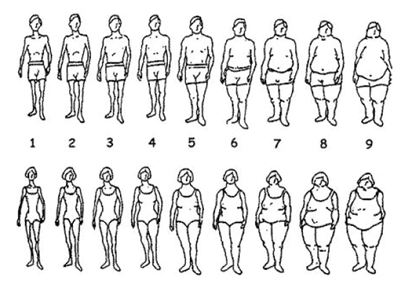
\includegraphics{percepcao-da-imagem-corporal-do-estudante-01.jpg}

}

\caption{Escala de Stunkard}

\end{figure}%

Neste exemplo, vamos analisar o recorte dos resultados para alunos entre
16 e 17 anos, diferenciando entre os sexos. As frequências estão
sumariadas na tabela abaixo.

\[\begin{array}{c|ccc|c}\hline
&\hbox{Satisfeito} & \hbox{Insatisfeito por excesso} & \hbox{Insatisfeito por magreza} &\hbox{Total}\\ \hline
\hbox{Masculino} & 24 & 10 & 24 & 58 \\
\hbox{Feminino} & 14 & 22 & 24 & 60 \\ \hline
\end{array}
\] Cada estudante pode assumir uma das três classificações. Sejam
\(\alpha_S,\alpha_E,\alpha_M\) as probabilidades de alguém do sexo
masculino estar classificado como Satisfeito, Insatisfeito por Excesso
ou Insatisfeito por magreza, respectivamente. Então a função de
verossimilhança para \(\boldsymbol{\alpha}\) é

\[L(\boldsymbol{\alpha})=\alpha_S^{24}\alpha_E^{10}\alpha_M^{24}.\]
Analogamente, fazendo \(\boldsymbol{\beta}=(\beta_S,\beta_E,\beta_M)\),
as mesmas probabilidades para o sexo feminino, teremos que

\[L(\boldsymbol{\alpha})=\beta_S^{14}\beta_E^{22}\beta_M^{24}.\]

Utilizando a priori Dirichlet(1,1,1) tanto para \(\boldsymbol{\alpha}\)
quanto para \(\boldsymbol{\beta}\), teremos que as respectivas
posterioris para \(\boldsymbol{\alpha}\) e \(\boldsymbol{\beta}\) são
Dirichelt(25,11,25) e Dirichlet(15,23,25).

As posterioris para \(\alpha_M\) e \(\beta_M\) e são Beta(25,36)
Beta(25,38). As estimativas pontuais são 0,40 e 0,39, respectivamente. A
imagem abaixo mostra a insatisfação por magreza entre os sexos deve ser
a mesma.

\begin{Shaded}
\begin{Highlighting}[]
\FunctionTok{curve}\NormalTok{(}\FunctionTok{dbeta}\NormalTok{(x,}\DecValTok{25}\NormalTok{,}\DecValTok{36}\NormalTok{), }\AttributeTok{lwd=}\DecValTok{2}\NormalTok{, }\AttributeTok{xlab =} \StringTok{\textquotesingle{}Probabilidade de insatisfação por magreza\textquotesingle{}}\NormalTok{, }\AttributeTok{ylab=} \StringTok{\textquotesingle{}Densidades marginais a posteriori\textquotesingle{}}\NormalTok{, }\AttributeTok{ylim=}\FunctionTok{c}\NormalTok{(}\DecValTok{0}\NormalTok{,}\DecValTok{8}\NormalTok{),}\AttributeTok{xlim=}\FunctionTok{c}\NormalTok{(.}\DecValTok{1}\NormalTok{,.}\DecValTok{8}\NormalTok{),}\AttributeTok{col=}\StringTok{\textquotesingle{}blue\textquotesingle{}}\NormalTok{)}
\FunctionTok{curve}\NormalTok{(}\FunctionTok{dbeta}\NormalTok{(x,}\DecValTok{25}\NormalTok{,}\DecValTok{38}\NormalTok{),}\AttributeTok{add =}\NormalTok{ T, }\AttributeTok{lwd=}\DecValTok{2}\NormalTok{, }\AttributeTok{col=}\StringTok{\textquotesingle{}red\textquotesingle{}}\NormalTok{)}
\FunctionTok{text}\NormalTok{(}\FunctionTok{c}\NormalTok{(.}\DecValTok{6}\NormalTok{,.}\DecValTok{2}\NormalTok{),}\FunctionTok{c}\NormalTok{(}\DecValTok{6}\NormalTok{,}\DecValTok{6}\NormalTok{), }\FunctionTok{c}\NormalTok{(}\StringTok{\textquotesingle{}Masculino\textquotesingle{}}\NormalTok{,}\StringTok{\textquotesingle{}Feminino\textquotesingle{}}\NormalTok{),}\AttributeTok{col=}\FunctionTok{c}\NormalTok{(}\StringTok{\textquotesingle{}blue\textquotesingle{}}\NormalTok{,}\StringTok{\textquotesingle{}red\textquotesingle{}}\NormalTok{))}
\end{Highlighting}
\end{Shaded}

\includegraphics{bernoulli_files/figure-pdf/unnamed-chunk-7-1.pdf}

As posterioris para \(\alpha_E\) e \(\beta_E\) são Beta(11,50)e
Beta(23,40). As estimativas pontuais são 0,21 e 0,36, respectivamente. A
imagem abaixo mostra que as mulheres em geral parecem possuir maior
probabilidade de insatisfação por excesso.

\begin{Shaded}
\begin{Highlighting}[]
\FunctionTok{curve}\NormalTok{(}\FunctionTok{dbeta}\NormalTok{(x,}\DecValTok{11}\NormalTok{,}\DecValTok{50}\NormalTok{), }\AttributeTok{lwd=}\DecValTok{2}\NormalTok{, }\AttributeTok{xlab =} \StringTok{\textquotesingle{}Probabilidade de insatisfação por excesso\textquotesingle{}}\NormalTok{, }\AttributeTok{ylab=} \StringTok{\textquotesingle{}Densidades marginais a posteriori\textquotesingle{}}\NormalTok{, }\AttributeTok{ylim=}\FunctionTok{c}\NormalTok{(}\DecValTok{0}\NormalTok{,}\DecValTok{10}\NormalTok{),}\AttributeTok{xlim=}\FunctionTok{c}\NormalTok{(}\DecValTok{0}\NormalTok{,.}\DecValTok{6}\NormalTok{))}
\FunctionTok{curve}\NormalTok{(}\FunctionTok{dbeta}\NormalTok{(x,}\DecValTok{23}\NormalTok{,}\DecValTok{40}\NormalTok{),}\AttributeTok{add =}\NormalTok{ T, }\AttributeTok{lwd=}\DecValTok{2}\NormalTok{)}
\FunctionTok{text}\NormalTok{(}\FunctionTok{c}\NormalTok{(.}\DecValTok{2}\NormalTok{,.}\DecValTok{4}\NormalTok{),}\FunctionTok{c}\NormalTok{(}\DecValTok{9}\NormalTok{,}\DecValTok{7}\NormalTok{), }\FunctionTok{c}\NormalTok{(}\StringTok{\textquotesingle{}Masculino\textquotesingle{}}\NormalTok{,}\StringTok{\textquotesingle{}Feminino\textquotesingle{}}\NormalTok{))}
\end{Highlighting}
\end{Shaded}

\includegraphics{bernoulli_files/figure-pdf/unnamed-chunk-8-1.pdf}

Podemos então construir a hipótese \(H:\alpha_E<\beta_E\). Abaixo,
testamos essa hipótese:

\begin{Shaded}
\begin{Highlighting}[]
\FunctionTok{set.seed}\NormalTok{(}\DecValTok{123}\NormalTok{)}
\NormalTok{B }\OtherTok{\textless{}{-}} \DecValTok{1000000}
\NormalTok{alfaE }\OtherTok{\textless{}{-}} \FunctionTok{rbeta}\NormalTok{(B, }\DecValTok{11}\NormalTok{,}\DecValTok{50}\NormalTok{)}
\NormalTok{betaE }\OtherTok{\textless{}{-}} \FunctionTok{rbeta}\NormalTok{(B, }\DecValTok{23}\NormalTok{,}\DecValTok{40}\NormalTok{)}
\FunctionTok{mean}\NormalTok{(alfaE}\SpecialCharTok{\textless{}}\NormalTok{betaE)}
\end{Highlighting}
\end{Shaded}

\begin{verbatim}
[1] 0.990628
\end{verbatim}

Com uma probabilidade maior que 99\%, há fortes evidências de que
mulheres entre 16 e 17 anos se sentem mais insatisfeitas por excesso do
que os homens de mesma idade.

\end{example}

\begin{example}[]\protect\hypertarget{exm-}{}\label{exm-}

\textbf{Imagem corporal (continuação)}

Neste exemplo, lidaremos apenas com o recorte dos indivíduos do sexo
masculino entre 16 e 17 anos, reproduzido abaixo.

\[\begin{array}{c|ccc|c}\hline
&\hbox{Satisfeito} & \hbox{Insatisfeito por excesso} & \hbox{Insatisfeito por magreza} &\hbox{Total}\\ \hline
\hbox{Masculino} & 24 & 10 & 24 & 58 \\ \hline
\end{array}
\]

Considerando \(\boldsymbol{alpha}=(\alpha_S,\alpha_E,\alpha_M)\) como
definidos anteriormente e utilizando a priori Dirichlet(1,1,1),
obtivemos a posteriori
\(\boldsymbol{\alpha}\sim\hbox{Dirichlet}(25,11,25)\).

Vamos testar se a probabilidade de insatisfação por magreza é maior do
que a por excesso, ou seja \(H: \alpha_M>\alpha_E\).

\begin{Shaded}
\begin{Highlighting}[]
\CommentTok{\#install.packages(\textquotesingle{}extraDistr\textquotesingle{})}
\FunctionTok{require}\NormalTok{(extraDistr)}
\end{Highlighting}
\end{Shaded}

\begin{verbatim}
Carregando pacotes exigidos: extraDistr
\end{verbatim}

\begin{verbatim}
Warning: pacote 'extraDistr' foi compilado no R versão 4.4.3
\end{verbatim}

\begin{Shaded}
\begin{Highlighting}[]
\NormalTok{B }\OtherTok{\textless{}{-}} \DecValTok{10000}
\NormalTok{alpha }\OtherTok{\textless{}{-}} \FunctionTok{rdirichlet}\NormalTok{(B, }\FunctionTok{c}\NormalTok{(}\DecValTok{25}\NormalTok{,}\DecValTok{11}\NormalTok{,}\DecValTok{25}\NormalTok{))}
\FunctionTok{mean}\NormalTok{( alpha[,}\DecValTok{3}\NormalTok{] }\SpecialCharTok{\textgreater{}}\NormalTok{ alpha[,}\DecValTok{2}\NormalTok{])}
\end{Highlighting}
\end{Shaded}

\begin{verbatim}
[1] 0.9893
\end{verbatim}

Com uma probabilidade maior que 0,99, existem fortes evidências de que,
para um indivíduo do sexo masculino entre 16 e 17 anos, a probabilidade
de estar insatisfeito por excesso é menor do que por magreza.

\end{example}

\section{Exercícios}\label{exercuxedcios}

\subsection{Eficácia de um Novo
Medicamento}\label{eficuxe1cia-de-um-novo-medicamento}

Uma empresa farmacêutica desenvolveu um novo medicamento para tratar
enxaquecas. Antes do lançamento, eles afirmam que o medicamento alivia a
dor em pelo menos 80\% dos pacientes. Um estudo independente com 250
pacientes revelou que 180 deles relataram alívio da dor. Os resultados
do estudo fornecem evidências suficientes para rejeitar a alegação da
empresa farmacêutica?

\subsection{Preferência por uma Marca de
Café}\label{preferuxeancia-por-uma-marca-de-cafuxe9}

Uma pesquisa de mercado afirma que 55\% dos consumidores preferem a
marca A de café à marca B. Uma amostra aleatória de 300 consumidores
revelou que 180 deles preferem a marca A. Os resultados da amostra
fornecem evidências suficientes para rejeitar a alegação da pesquisa de
mercado?

\subsection{Taxa de Aprovação em um
Exame}\label{taxa-de-aprovauxe7uxe3o-em-um-exame}

Uma escola afirma que a taxa de aprovação em um exame padronizado é de
70\%. Uma amostra de 200 alunos revelou que 120 deles foram aprovados.
Os resultados da amostra fornecem evidências suficientes para rejeitar a
alegação da escola?

\subsection{Eficácia de uma Campanha de
Vacinação}\label{eficuxe1cia-de-uma-campanha-de-vacinauxe7uxe3o}

Uma campanha de vacinação contra a gripe foi realizada em uma cidade.
Antes da campanha, a taxa de vacinação era de 35\%. Após a campanha, uma
amostra de 400 pessoas revelou que 180 delas foram vacinadas. Os
resultados da amostra fornecem evidências suficientes para concluir que
a campanha aumentou a taxa de vacinação?

\subsection{A eficácia da Pfizer}\label{a-eficuxe1cia-da-pfizer}

O artigo Polack et al. (2020) apresenta um estudo clínico de fase 3
randomizado e controlado por placebo que avaliou a eficácia da vacina
BNT162b2 (Pfizer-BioNTech COVID-19) em participantes com 16 anos ou mais
sem evidências de infecção por SARS-CoV-2. A tabela abaixo apresenta o
número de participantes por grupo e o número de casos de Covid-19.

\[\begin{array}{l|cc}\hline
\hbox{Grupo} & \hbox{Participantes} & \hbox{Casos de Covid-19}\\\hline
\hbox{Vacina} & 18.198 & 8 \\
\hbox{Placebo} & 18.325 & 162 \\ \hline
\end{array}\]

Considere que o evento de interesse é contrair Covid-19

\begin{itemize}
\item
  Encontre a função de verossimilhança para cada grupo
\item
  Utilizando a priori Beta(1,1) para a probabilidade de contrair
  Covid-19, encontre a distribuição a posteriori para cada grupo
\item
  Faça um gráfico das posterioris e verifique se há evidências de que a
  vacinação é eficaz.
\end{itemize}

\subsection{O Naufrágio do Lusitania
(1915)}\label{o-naufruxe1gio-do-lusitania-1915}

Neste capítulo, abordamos a tragédia do Lusitania. A tabela abaixo
acrescenta os dados sobre a tripulação.

\[\begin{array}{l|cc} \hline
\hbox{Categoria} & \hbox{Sobreviventes} & \hbox{Mortos} \\ \hline
\hbox{Primeira classe} & 113 & 177 \\
\hbox{Segunda classe} & 229 & 372 \\ 
\hbox{Terceira classe}  & 134 & 239 \\ \hline
\hbox{Tripulação - abastecimento} & 139 & 167 \\
\hbox{Tripulação - engenharia} & 112 & 201 \\
\hbox{Tripulação - deck} & 41 & 37 \\
\hline
\end{array}\]

Compare a probabilidade de sobrevivência entre os indivíduos dos
diferentes tipos de tripulação e classes de passageiros, testando as
hipóteses necessárias.

\subsection{Imagem corporal}\label{imagem-corporal}

Neste capítulo, mostramos que homens e mulheres com idades entre 16 e 17
anos possuem expectativas diferentes em relação ao seu próprio corpo.

Neste exercício, você vai verificar como essas expectativas variam
dentro do mesmo sexo. Especificamente:

\begin{itemize}
\item
  Teste se há evidências de que os homens possuem probabilidade maior de
  estarem insatisfeitos por magreza do que satisfeitos.
\item
  Teste se há evidências de que as mulheres possuem probabilidade maior
  de estarem insatisfeitas por excesso do que satisfeitas.
\end{itemize}

\bookmarksetup{startatroot}

\chapter{Testes de hipóteses}\label{testes-de-hipuxf3teses}

\section{Testes baseados na teoria da
decisão}\label{testes-baseados-na-teoria-da-decisuxe3o}

\subsection{A Função de Perda 0-1}\label{a-funuxe7uxe3o-de-perda-0-1}

Considere que \(X_1,\ldots,X_n\) é uma amostra do modelo
\(F(.|\theta)\). Seja \(H_0:\theta\in\Theta_0\) a hipótese nula.

Um teste de hipóteses é uma regra \(\varphi(x)\) que recebe o valor 1 se
a hipótese \(H_0\) é aceita e 0 em caso contrário.

Em relação à natureza da hipótese, observe que
\[I(\theta\in\Theta_0)=\left\{\begin{array}{ll}1,&\hbox{ se }H_0\hbox{ é verdadeira}\\0,&\hbox{ se }H_0\hbox{ é falsa}\end{array}\right..\]

Novamente, considere a função de perda quadrática:

\[ \mathcal{L}(\theta,\varphi)=(\varphi(x)-I(\theta\in\Theta_0))^2.\]
Definida deste modo, esta função também é denominada Função de Perda
0-1, uma vez que ela assume o valor 0 quando uma decisão correta é
tomada e 1 caso contrário.

A esperança a posteriori desta função de perda é

\[E_{\theta|X}(\mathcal{L}(\theta,\varphi))=\int \left(\phi(x)- I(\theta\in\Theta_0)\right)^2 f(\theta|x)d\theta\]

e o estimador de Bayes é o valor de \(\varphi\) que minimiza a esperança
acima. Como \(\varphi\) é uma indicadora, teremos duas situações:

\begin{itemize}
\tightlist
\item
  Se \(\phi(x)=0\), então
\end{itemize}

\[\begin{align}E_{\theta|X}(\mathcal{L}(\theta,\varphi))&=\int I(\theta\in\Theta_0)^2 f(\theta|x)d\theta\\&=\int I(\theta\in\Theta_0) f(\theta|x)d\theta\\&=\int_{\Theta_0 }f(\theta|x)d\theta=P(\theta\in\Theta_0|x)\end{align}\]

\begin{itemize}
\tightlist
\item
  Se \(\phi(x)=1\), então
\end{itemize}

\[\begin{align}E_{\theta|X}(\mathcal{L}(\theta,\varphi))&=\int (1-I(\theta\in\Theta_0)^2 f(\theta|x)d\theta\\&=\int I(\theta\in\Theta_0^c) f(\theta|x)d\theta\\&=\int_{\Theta_0^c }f(\theta|x)d\theta=P(\theta\notin\Theta_0|x)\end{align}\]

Deste modo, se \(P(\theta\in\Theta_0|x)>P(\theta\in\Theta_0^c|x)\),
temos que \(\phi(\boldsymbol{x})=1\) é a decisão que minimiza a perda a
posteriori, ou seja, aceitamos \(H_0\). Em caso contrário, rejeitamos
\(H_0\).

\begin{example}[]\protect\hypertarget{exm-}{}\label{exm-}

Fast food

Uma cadeia de \emph{fast food} deseja saber se vale a pena trocar seus
freezers tradicionais, que mantém a carne entre -\(17^o\)C e \(-9^oC\)
por um com uma nova tecnologia (e mais cara!) que mantém a temperatura
consistentemente em \(-17^oC\). Para tomar essa decisão, 32 bifes foram
armazenados por 8 meses, sendo 16 bifes colocados no freezer tradicional
e 16 no novo. Em seguida, um chefe preparou os 32 bifes de maneira
idêntica e 16 clientes foram escolhidos ao acaso para avaliar o sabor
dos bifes. Cada cliente recebeu um bife de cada freezer, mas a prova foi
realizada às cegas.

Podemos considerar a variável \(Y_i=1\) se o \(i\)-ésimo cliente
preferiu o bife armazenado no freezer mais caro e \(Y_i=0\) em caso
contrário. Deste modo,
\(Y_1,\ldots,Y_{16}|\theta\sim\hbox{Bernoulli}(\theta)\). Claramente,
estamos interessados em testar \(H_0:\theta>1/2\).

Considere as seguintes prioris:

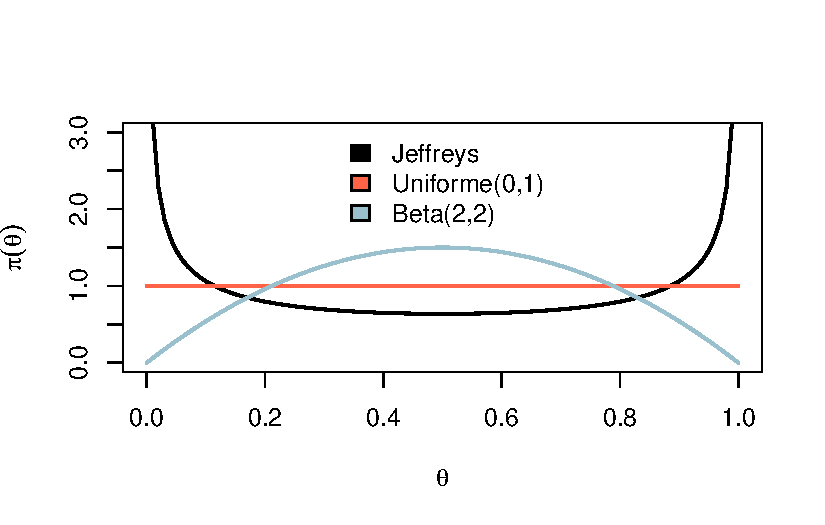
\includegraphics{teste_files/figure-pdf/unnamed-chunk-1-1.pdf}

A distribuiação a priori Beta(.5,.5) dá mais massa para valores
extremos, o que poderia favorecer a hipótese \(H_0\). A priori Beta(1,1)
é aquela que parece não dar qualquer preferência. Por último, a priori
Beta(2,2) pode ser vista como uma leve resistência à rejeitar que os
dois armazenamentos são iguais.

Dos 16 clientes, 13 preferiram os bifes que foram armazenados com a
tecnologia mais cara. Como as três prioris acima são casos particulares
da distribuição Beta\((a,b)\), decidiremos sobre \(H_0\) calculando

\[P(\theta>1/2|\textbf{y})=\int_0^{1/2}\frac{\theta^{13+a-1}(1-\theta)^{3+b-1}}{B(13+a,3+b)}\]

que pode ser facilmente obtida com o comando
\texttt{pbeta(.5,13+a,3+b,\ lower.tail\ =F)} Temos os seguintes
resultados:

\begin{longtable}[]{@{}ll@{}}
\toprule\noalign{}
Priori & \(P(H_0|\textbf{y})\) \\
\midrule\noalign{}
\endhead
\bottomrule\noalign{}
\endlastfoot
Beta(.5,.5) & 0,995 \\
Uniforme & 0,993 \\
Beta(2,2) & 0,990 \\
\end{longtable}

Considerando as prioris acima, a probabilidade a posteriori da hipótese
nula é de pelo menos 0,99, o que nos leva a concluir que o sabor da
carne é melhor preservado no freezer com alta tecnologia

\end{example}

\subsection{A Função de Perda a-b}\label{a-funuxe7uxe3o-de-perda-a-b}

Suponha que \(P(\theta\in\Theta_0|\boldsymbol{x})=0,51\). Segundo a
Função de Perda 0-1, deveríamos aceitar \(H_0\), uma vez que

\[P(\theta\in\Theta_0|\boldsymbol{x})=0,51>0,49=P(\theta\in\Theta_0^c|\boldsymbol{x})\]

Isto ocorre porque a perda associada ao erro no teste de hipóteses é
igual para qualquer decisão. Podemos associar valores diferentes,
reforçando que um erro é mais sério que o outro.

Considere que rejeitar \(H_0\) quando ela é verdadeira (erro tipo I)
gera uma perda \(a\), enquanto que aceitar \(H_0\) quando ela é falsa
(erro tipo II) gera uma perda \(b\). Para o erro mais grave, associamos
um valor maior para a perda. A função de perda respectiva é denominada
Perda \(a-b\) e é dada por

\[\mathcal{L}(\theta,\varphi)=\left\{\begin{array}{l}0,\hbox{ se }\varphi(x)=I(\theta\in\Theta_0)\\
a,\hbox{ se }\varphi(x)=0\hbox{ e }\theta\in\Theta_0\\b,\hbox{ se }\varphi(x)=1\hbox{ e }\theta\notin\Theta_0\end{array}\right.\]

A média a posteriori dessa função de perda é

\[E_{\theta|\boldsymbol{x}}(\mathcal{L}(\theta,\varphi))=a\int_{\Theta_0}I(\varphi(x)=0)f(\theta|x)d\theta+b\int_{\Theta_0^c}I(\varphi(x)=1)f(\theta|x)d\theta\]

\begin{itemize}
\item
  Se \(\varphi(x)=1\), teremos
  \[E_{\theta|x}(\mathcal{L}(\theta,\varphi))=b\int_{\Theta_0^c}I(\varphi(x)=1)f(\theta|\boldsymbol{x})d\theta=bP(\theta\in\Theta_0^c|x)\]
\item
  Se \(\varphi(x)=0\) teremos
  \[E_{\theta|x}(\mathcal{L}(\theta,\varphi))=a\int_{\Theta_0}I(\varphi(x)=0)f(\theta|x)d\theta=aP(\theta\in\Theta_0|x)\]
  logo:
\item
  Se \(bP(\theta\in\Theta_0^c|x)>aP(\theta\in\Theta_0|x)\) então a
  decisão minimiza a perda a posteriori é \(\varphi(\boldsymbol{x})=0\),
  ou seja, rejeitamos \(H_0\).
\item
  Se \(bP(\theta\in\Theta_0^c|x)<aP(\theta\in\Theta_0|x)\) então a
  decisão minimiza a perda a posteriori é \(\varphi(\boldsymbol{x})=1\),
  ou seja, aceitamos \(H_0\).
\end{itemize}

Na prática, aceitamos \(H_0\) se
\[P(\theta\in\Theta_0|\boldsymbol{x})>\frac{b}{b+a}\]

Observe que, diferente do ponto de vista frequentista, estamos
interessados em aceitar a hipótese \(H_0\). Deste modo, o erro tipo II é
o mais preocupante, o que implica em \(b>a\). Na prática, fixamos um
valor para \(b/(a+b)\), como 0,95 ou 0,99 e comparamos com
\(P(\theta\in\Theta_0|\boldsymbol{x})\) para decidir se aceitamos
\(H_0\).

\begin{example}[]\protect\hypertarget{exm-}{}\label{exm-}

\textbf{Mudança de opinião}

Durante a eleição presidencial americana de 1980 um estudo foi conduzido
para determinar se um debate televisionado foi capaz de mudar as
preferências dos telespectadores pelos candidatos. Foram selecionados 75
adultos aleatoriamente e sua preferência entre os dois candidatos foi
registrada. Após a conclusão do detabe, foi perguntado para as mesmas 75
pessoas a sua preferência entre os dois candidatos. Os resultados estão
sumariados abaixo.

\[\begin{array}{c|c|c}\hline
\text{Preferência antes } & \text{Preferência depois} & \text{Resultado} \\  
\text{do debate} & \text{do debate} & \\ \hline
\text{Carter} & \text{Carter} & 28 \\
\text{Carter} & \text{Reagan} & 13 \\
\text{Reagan} & \text{Reagan} & 27 \\ 
\text{Reagan} & \text{Carter} & 7 \\ \hline
\end{array}\]

Neste exemplo, vamos testar se os dois candidatos foram igualmente
capazes de mudar a opinião dos eleitores.

Sabemos que 20 eleitores mudaram de opinição

\begin{itemize}
\item
  \(\theta_{CC}\): a probabilidade do indivíduo preferir o candidato
  Carter antes de depois do debate
\item
  \(\theta_{RR}\): a probabilidade do indivíduo preferir o candidato
  Reagan antes de depois do debate
\item
  \(\theta_{CR}\): a probabilidade do indivíduo preferir o candidato
  Carter e depois mudar para o Reagan.
\item
  \(\theta_{RC}\): a probabilidade do indivíduo preferir o candidato
  Reagan e depois mudar para o Carter.
\end{itemize}

A função de verossimilhança para
\(\boldsymbol{\theta}=(\theta_{CC},\theta_{CR},\theta_{RC},\theta_{RR})\)
é

\[L(\boldsymbol{\theta})\propto \theta_{CC}^{28}\theta_{CR}^{13}\theta_{RR}^{27}\theta_{RC}^{7}.\]

Considerando a priori
\(\boldsymbol{\theta}\sim\hbox{Dirichlet}(1,1,1,1)\), teremos a
posteriori

\[\boldsymbol{\theta}\sim\hbox{Dirichlet}(29,14,28,8),\]

Estamos interessados nas probabilidades sobre mudança de opinião, ou
seja, em \(\theta_{CR}\) e \(\theta_{RC}\), cujas posterioris são
\[\begin{align}
\theta_{CR}&\sim\hbox{Beta}(14,65)\\
\theta_{RC}&\sim\hbox{Beta}(7,68)
\end{align}\]

Abaixo, apresentamos as posterioris de \(\theta_{CR}\) e
\(\theta_{RC}\). Pode-se observar que o candidato Reagan parece ter
certa vantagem.

\begin{Shaded}
\begin{Highlighting}[]
\FunctionTok{curve}\NormalTok{(}\FunctionTok{dbeta}\NormalTok{(x,}\DecValTok{14}\NormalTok{,}\DecValTok{65}\NormalTok{), }\AttributeTok{ylim=}\FunctionTok{c}\NormalTok{(}\DecValTok{0}\NormalTok{,}\DecValTok{15}\NormalTok{), }\AttributeTok{xlim=}\FunctionTok{c}\NormalTok{(}\DecValTok{0}\NormalTok{,.}\DecValTok{5}\NormalTok{), }\AttributeTok{xlab=} \StringTok{\textquotesingle{}Probabilidade de mudança\textquotesingle{}}\NormalTok{, }\AttributeTok{ylab=}\StringTok{\textquotesingle{}Densidade a posteriori\textquotesingle{}}\NormalTok{, }\AttributeTok{lwd =} \DecValTok{2}\NormalTok{)}
\FunctionTok{curve}\NormalTok{(}\FunctionTok{dbeta}\NormalTok{(x,}\DecValTok{7}\NormalTok{,}\DecValTok{68}\NormalTok{), }\AttributeTok{add =}\NormalTok{ T, }\AttributeTok{lwd =} \DecValTok{2}\NormalTok{, }\AttributeTok{lty =} \DecValTok{2}\NormalTok{)}
\FunctionTok{legend}\NormalTok{(}\StringTok{\textquotesingle{}topright\textquotesingle{}}\NormalTok{,}\FunctionTok{c}\NormalTok{(}\StringTok{\textquotesingle{}Mudança em favor do Reagan\textquotesingle{}}\NormalTok{, }\StringTok{\textquotesingle{}Mudança em favor do Carter\textquotesingle{}}\NormalTok{), }\AttributeTok{lwd=}\DecValTok{2}\NormalTok{, }\AttributeTok{lty=}\DecValTok{1}\SpecialCharTok{:}\DecValTok{2}\NormalTok{, }\AttributeTok{bty=}\StringTok{\textquotesingle{}n\textquotesingle{}}\NormalTok{)}
\end{Highlighting}
\end{Shaded}

\includegraphics{teste_files/figure-pdf/unnamed-chunk-2-1.pdf}

Vamos testar se o debate do candidato Reagan foi mais eficaz para
provocar a mudança de opinião, ou seja, \(H:\theta_{RC}<\theta_{CR}\).

\begin{Shaded}
\begin{Highlighting}[]
\FunctionTok{require}\NormalTok{(extraDistr)}
\end{Highlighting}
\end{Shaded}

\begin{verbatim}
Carregando pacotes exigidos: extraDistr
\end{verbatim}

\begin{verbatim}
Warning: pacote 'extraDistr' foi compilado no R versão 4.4.3
\end{verbatim}

\begin{Shaded}
\begin{Highlighting}[]
\NormalTok{B }\OtherTok{\textless{}{-}} \DecValTok{20000}
\NormalTok{theta }\OtherTok{\textless{}{-}} \FunctionTok{rdirichlet}\NormalTok{(B, }\FunctionTok{c}\NormalTok{(}\DecValTok{29}\NormalTok{,}\DecValTok{14}\NormalTok{,}\DecValTok{28}\NormalTok{,}\DecValTok{8}\NormalTok{))}
\NormalTok{thetaCR }\OtherTok{\textless{}{-}}\NormalTok{ theta[,}\DecValTok{2}\NormalTok{]}
\NormalTok{thetaRC }\OtherTok{\textless{}{-}}\NormalTok{ theta[,}\DecValTok{4}\NormalTok{]}
\FunctionTok{mean}\NormalTok{(thetaRC }\SpecialCharTok{\textless{}}\NormalTok{ thetaCR)}
\end{Highlighting}
\end{Shaded}

\begin{verbatim}
[1] 0.90305
\end{verbatim}

Não há evidência forte o suficiente para aceitar a superioridade do
Reagan para a mudança de opinião. Abaixo, mostramos o gráfico estimado
para a posteriori de \(\theta_{CR},\theta_{RC}\).

\begin{Shaded}
\begin{Highlighting}[]
\FunctionTok{require}\NormalTok{(MASS)}
\end{Highlighting}
\end{Shaded}

\begin{verbatim}
Carregando pacotes exigidos: MASS
\end{verbatim}

\begin{Shaded}
\begin{Highlighting}[]
\FunctionTok{contour}\NormalTok{(}\FunctionTok{kde2d}\NormalTok{(thetaCR,thetaRC), }\AttributeTok{xlab=}\FunctionTok{expression}\NormalTok{(theta[CR]),}\AttributeTok{ylab=}\FunctionTok{expression}\NormalTok{(theta[RC]), }\AttributeTok{lwd =} \DecValTok{2}\NormalTok{)}
\FunctionTok{abline}\NormalTok{(}\DecValTok{0}\NormalTok{,}\DecValTok{1}\NormalTok{,}\AttributeTok{lty=}\DecValTok{2}\NormalTok{, }\AttributeTok{lwd =} \DecValTok{2}\NormalTok{)}
\end{Highlighting}
\end{Shaded}

\includegraphics{teste_files/figure-pdf/unnamed-chunk-4-1.pdf}

\end{example}

\section{Testes utilizando modelos}\label{testes-utilizando-modelos}

Considere novamente o problema dos freezers, da seção anterior. Note que
a teoria desenvolvida acima não consegue testar \(H_0:\theta=1/2\), uma
vez que este evento possui probabilidade nula a priori.

Para contornar este problema, suponha que existem dois modelos
concorrentes:

\begin{itemize}
\item
  Modelo \(M_0\): \(y_i\sim\hbox{Bernoulli}(1/2)\)
\item
  Modelo \(M_1:\)
\end{itemize}

\[\begin{align}
y_i|\theta&\sim\hbox{Bernoulli}(\theta),\\
\theta&\sim\hbox{Uniforme}(0,1)\end{align}\]

Seja \(M_0\) o evento no qual o modelo \(M_0\) é o verdadeiro gerador da
amostra. Observe que
\[f(y_1,\ldots,y_{16}|M_0)=\prod_{i=1}^{16}f(y_i|M_0)=\left(\frac{1}{2}\right)^{16}\]

Já para o modelo \(M_1\), observe que

\[\begin{align}f(y_1,\ldots,y_{16}|M_1)&=
\int_0^1 f(y_1,\ldots,y_{16}|\theta)f(\theta)d\theta\\
&=\int_0^1 \prod_{i=1}^{16}f(y_i|\theta)f(\theta)d\theta\\
&=\int_0^1 \prod_{i=1}^{16}\theta^{y_i}(1-\theta)^{1-y_i}d\theta\\
&=\int_0^1\theta^{\sum_{i=1}^{16}y_i}(1-\theta)^{16-\sum_{i=1}^{16}y_i}d\theta=B\left(\sum_{i=1}^{16}y_i+1,16-\sum_{i=1}^{16}y_i+1\right),\end{align}\]
onde \(B(.,.)\) é a função beta.

Sejam \(P(M_0)\) e \(P(M_1)=1-P(M_0)\) as probabilidades a priori dos
modelos \(M_0\) e \(M_1\). Então, a probabilidade a posteriori do modelo
\(M_0\) é dada por

\[P(M_0|y_1,\ldots,y_{16})=\frac{\left(\frac{1}{2}\right)^{16}P(M_0)}{\left(\frac{1}{2}\right)^{16}P(M_0)+B\left(\sum_{i=1}^{16}y_i+1,16-\sum_{i=1}^{16}y_i+1\right)P(M_1)}\]
Ainda considerando o exemplo anterior, assumindo \(P(M_0)=P(M_1)=1/2\) e
lembrando que \(\sum_i y_i=13\), tem-se

\[P(M_0|y_1,\ldots,y_{16})=\frac{\left(\frac{1}{2}\right)^{17}}{\left(\frac{1}{2}\right)^{17}+B\left(14,4\right)\frac{1}{2}}\approx0,1268,\]
o que nos leva a rejeitar \(H_0\).

\textbf{Caso geral.}

Para a amostra \(x_1,\ldots,x_n\), sejam \(M_1,\ldots,M_k\) \(k\)
modelos paramétricos. Sejam
\(\boldsymbol{\theta}_1,\ldots,\boldsymbol{\theta}_k\), e
\(f(\boldsymbol{\theta}_1),\ldots,f(\boldsymbol{\theta}_k)\) seus
respectivos parâmetros e prioris. Para determinar o modelo mais
adequado:

\begin{enumerate}
\def\labelenumi{\arabic{enumi}.}
\item
  Atribua os valores a priori para \(P(M_1),\ldots,P(M_k)\)
\item
  Para \(j=1,\ldots,k\), calcule
  \[f(x_1,\ldots,x_n|M_j)=\int f(x_1,\ldots,x_n|\theta_j)f_j(\theta_j)d\theta_j\]
\item
  Compute
\end{enumerate}

\[P(M_j|x_1,\ldots,x_n)=\frac{f(x_1,\ldots,x_n|M_j)P(M_j)}{\sum_{i=1}^k f(x_1,\ldots,x_n|M_i)P(M_i)}\]

\begin{enumerate}
\def\labelenumi{\arabic{enumi}.}
\setcounter{enumi}{3}
\tightlist
\item
  Considere como adequado o modelo com maior probabilidade a posteriori
\end{enumerate}

\textbf{Distribuição preditiva para o caso Bernoulli multivariado}

A distribuição \[f(x)=\int L(\theta)f(\theta)d\theta=E(L(\theta))\] é
denominada preditiva. Se
\(\boldsymbol{X}|\boldsymbol{\theta}\sim\hbox{Bernoulli}(\theta_1,\ldots,\theta_k)\)
e considerando o modelo conjugado
\(\boldsymbol{\theta}\sim\hbox{Dirichlet}(\theta_1,\ldots,\theta_k)\),
teremos que

\[\begin{align}
f(x)&=\int_{\mathcal{S}^k}\prod_{j=1}^k\theta_j^{n_j}\frac{\Gamma(\sum_{j=1}^k a_j)}{\prod_{j=1}^k \Gamma(a_j)}\prod_{j=1}^k \theta_j^{a_j-1}d\boldsymbol{\theta}\\
&=\frac{\Gamma(\sum_{j=1}^k a_j)}{\prod_{j=1}^k \Gamma(a_j)}\int_{\mathcal{S}^k}\prod_{j=1}^k\theta_j^{n_j+a_j-1}d\boldsymbol{\theta}\\
&=\frac{\Gamma(\sum_{j=1}^k a_j)}{\Gamma(n+\sum_{j=1}^k a_j)}\prod_{j=1}^k\frac{\Gamma(a_j+n_j)}{\Gamma(a_j)}
\end{align}\]

Além disso, se \(a_1=\cdots=a_k=1\), então

\[f(x)=\frac{(k-1)!}{(n+k-1)!}\prod_{j=1}^k n_j!\]

\begin{example}[]\protect\hypertarget{exm-}{}\label{exm-}

\textbf{Imagem corporal}

Considere novamente os dados sobre imagem corporal em escolares entre 16
e 17 anos, vistos no capítulo anterior e reproduzidos novamente abaixo.

vamos analisar o recorte dos resultados para alunos entre 16 e 17 anos,
diferenciando entre os sexos. As frequências estão sumariadas na tabela
abaixo.

\[\begin{array}{c|ccc|c}\hline
&\hbox{Satisfeito} & \hbox{Insatisfeito por excesso} & \hbox{Insatisfeito por magreza} &\hbox{Total}\\ \hline
\hbox{Masculino} & 24 & 10 & 24 & 58 \\
\hbox{Feminino} & 14 & 22 & 24 & 60 \\ \hline
\end{array}
\]

Anteriormente, assumimos que as probabilidades entre os sexos deveriam
ser diferentes. Denotamos por \(\alpha_S,\alpha_E,\alpha_M\) a
probabilidade de um indivíduo do sexo masculino ser classificado como
Satisfeito, Insatisfeito por Excesso e Insatisfeito por Magreza. Também
denotamos por \(\beta_S,\beta_E,\beta_M\) as mesmas probabilidades para
o sexo feminino. Por último, Utilizamos a priori Dirichlet(1,1,1) para
ambos os sexos. Vamos denotar esse modelo por \(M_1\).

Seja \(x=(24,10,24)\) as informações registradas para o sexo masculino e
\(y=(14,22,24)\) as informações para o sexo feminino. Então

\[\begin{align}
f(x,y|M_1)&=f(x|M_1)f(y|M_1)\\
&=\left[\frac{2!}{60!}24!10!24!\right]\left[\frac{2!}{62!}14!22!24!\right]
\end{align}\]

Considere agora o modelo \(M_2\), no qual não há diferença entre os
sexos. Nesse caso, \(x\) e \(y\) são provenientes do mesmo modelo, com
probabilidades \(\gamma_S,\gamma_E,\gamma_M\), respectivamente.
Utilizando a priori Dirichlet(1,1,1), teremos

\[\begin{align}f(x,y|M_2)&=\frac{2!}{120!}38!32!48!\end{align}\]

Vamos assumir a priori que \(P(M_1)=P(M_2)=1/2\). Então, vamos testar se
não há diferença na percepção da imagem corporal entre os sexos:

\[P(M_2|x,y)=\frac{P(x,y|M_2)}{P(x,y|M_1)+P(x,y|M_2)}\]

Vamos realizar esse cálculo no \texttt{R}:

\begin{itemize}
\tightlist
\item
  \(P(x,y|M_1)\):
\end{itemize}

\begin{Shaded}
\begin{Highlighting}[]
\CommentTok{\# logaritmo da probabilidade:}
\NormalTok{lprobA }\OtherTok{\textless{}{-}} \FunctionTok{lfactorial}\NormalTok{(}\DecValTok{2}\NormalTok{)}\SpecialCharTok{{-}}\FunctionTok{lfactorial}\NormalTok{(}\DecValTok{60}\NormalTok{)}\SpecialCharTok{+}\FunctionTok{sum}\NormalTok{(}\FunctionTok{lfactorial}\NormalTok{(}\FunctionTok{c}\NormalTok{(}\DecValTok{24}\NormalTok{,}\DecValTok{10}\NormalTok{,}\DecValTok{24}\NormalTok{)))}
\NormalTok{lprobB }\OtherTok{\textless{}{-}} \FunctionTok{lfactorial}\NormalTok{(}\DecValTok{2}\NormalTok{)}\SpecialCharTok{{-}}\FunctionTok{lfactorial}\NormalTok{(}\DecValTok{62}\NormalTok{)}\SpecialCharTok{+}\FunctionTok{sum}\NormalTok{(}\FunctionTok{lfactorial}\NormalTok{(}\FunctionTok{c}\NormalTok{(}\DecValTok{14}\NormalTok{,}\DecValTok{22}\NormalTok{,}\DecValTok{24}\NormalTok{)))}
\CommentTok{\# probabilidade}
\NormalTok{m1 }\OtherTok{\textless{}{-}} \FunctionTok{exp}\NormalTok{(lprobA }\SpecialCharTok{+}\NormalTok{lprobB)}
\end{Highlighting}
\end{Shaded}

\begin{itemize}
\tightlist
\item
  \(P(x,y|M_2)\):
\end{itemize}

\begin{Shaded}
\begin{Highlighting}[]
\CommentTok{\# logaritmo da probabilidade:}
\NormalTok{lprob }\OtherTok{\textless{}{-}} \FunctionTok{lfactorial}\NormalTok{(}\DecValTok{2}\NormalTok{)}\SpecialCharTok{{-}}\FunctionTok{lfactorial}\NormalTok{(}\DecValTok{120}\NormalTok{)}\SpecialCharTok{+}\FunctionTok{sum}\NormalTok{( }\FunctionTok{lfactorial}\NormalTok{(}\FunctionTok{c}\NormalTok{(}\DecValTok{38}\NormalTok{,}\DecValTok{32}\NormalTok{,}\DecValTok{48}\NormalTok{)))}
\CommentTok{\# probabilidade}
\NormalTok{m2 }\OtherTok{\textless{}{-}} \FunctionTok{exp}\NormalTok{(lprob)}
\end{Highlighting}
\end{Shaded}

\begin{itemize}
\tightlist
\item
  \(P(M_2|x,y)\)
\end{itemize}

\begin{Shaded}
\begin{Highlighting}[]
\NormalTok{m2 }\SpecialCharTok{/}\NormalTok{ (m1 }\SpecialCharTok{+}\NormalTok{ m2)}
\end{Highlighting}
\end{Shaded}

\begin{verbatim}
[1] 0.2824985
\end{verbatim}

Portanto, ficamos com o modelo que assume diferença entre os sexos.

\end{example}

\section{O Fator de Bayes}\label{o-fator-de-bayes}

Anteriormente, vimos que para uma coleção de \(k\) modelos competidores,
o modelo \(M_j\) é preferível aos demais se \[P(M_j|x)>P(M_i|x).\] para
todo \(i\neq j\). Observe que

\[\begin{align}P(M_j|x)&=\frac{f(x|M_j)P(M_j)}{\sum_{i=1}^kf(x|M_j)P(M_j)}\\&=P(M_j)\left[P(M_j)+\sum_{i\neq j}\frac{f(x|M_i)}{f(x|M_j)}P(M_i)\right]^{-1}\\
&=P(M_j)\left[P(M_j)+\sum_{i\neq j}B_{ij}(x)P(M_i)\right]^{-1}\end{align}\]
onde a quantidade \[B_{ij}(x)=\frac{f(x|M_i)}{f(x|M_j)},\] denominada
Fator de Bayes, sumariza a informação da amostra para relacionar os
modelo \(M_i\) e \(M_j\).

Para auxiliar na interpretação do Fator de Bayes, considere o caso com
apenas dois modelos onde \(P(M_1)=P(M_2)\). Então
\[\begin{align}P(M_1|x)&=
&=\left[1+B_{21}(x)\right]^{-1}\end{align}\] Observe que, quanto maior
for o valor \(B_{21}(x)\), menor será a evidência a favor do modelo
\(M_1\).

A escala de Jeffreys pode ser útil para tomada de decisão:

\[\begin{array}{cl}\hline B_{01}(x) & \text{Interpretação}\\ \hline
>100 & \text{Evidência decisiva para } H_0 \\
30-100 & \text{Evidência muito forte para } H_0 \\
10-30 & \text{Evidência forte para } H_0 \\
3-10 & \text{Evidência substancial para } H_0 \\
1-3 & \text{Evidência fraca para } H_0 \\
1/3-1 & \text{Evidência fraca contra } H_0 \\
1/10-1/3 & \text{Evidência substancial contra } H_0 \\
1/30-1/10 & \text{Evidência forte contra } H_0 \\
1/100-1/30 & \text{Evidência muito forte contra } H_0 \\
<1/100 & \text{Evidência decisiva contra } H_0 \\ \hline
\end{array}\]

Note que, se \(M_0\) é equivalente à \(\theta_0\) e \(M_1\) é
equivalente à \(\theta=\theta_1\), então o Fator de Bayes se torna a
estatística do teste de Neyman-Pearson

\[B_{01}(x)=\frac{f(x|\theta_0)}{f(x|\theta_1)}.\]

\begin{example}[]\protect\hypertarget{exm-}{}\label{exm-}

\textbf{Imagem corporal}

Considerando \(M_1\) como o modelo no qual as percepções sobre o corpo
são provenientes de populações distintas e \(M_2\) como o modelo no qual
não havia diferença entre os grupos delimitados pelo sexo, obtivemos
\(P(M_2|x,y)\approx 0,28\). Utilizando os mesmos comandos em \texttt{R},
teremos que o Fator de Bayes \(B_{21}\) é dado por

\begin{Shaded}
\begin{Highlighting}[]
\NormalTok{m2}\SpecialCharTok{/}\NormalTok{m1}
\end{Highlighting}
\end{Shaded}

\begin{verbatim}
[1] 0.3937254
\end{verbatim}

que gera evidência fraca em favor de \(M_1\).

\end{example}

\begin{example}[]\protect\hypertarget{exm-}{}\label{exm-}

\textbf{Pesquisa Quaest}

Uma pesquisa foi realizada entre os dias 27 e 31 de março de 2025 e
ouviu 2.024 eleitores presencialmente. Uma das perguntas foi: O quão
frustrado você está com o governo Lula hoje? As opções eram 1) Muito
frustrado, (2) Pouco frustrado, (3), Nada frustrado e (4) Não sabe/Não
respondeu.

\begin{longtable}[]{@{}
  >{\raggedright\arraybackslash}p{(\columnwidth - 4\tabcolsep) * \real{0.3014}}
  >{\centering\arraybackslash}p{(\columnwidth - 4\tabcolsep) * \real{0.3288}}
  >{\centering\arraybackslash}p{(\columnwidth - 4\tabcolsep) * \real{0.3699}}@{}}
\toprule\noalign{}
\begin{minipage}[b]{\linewidth}\raggedright
Categoria
\end{minipage} & \begin{minipage}[b]{\linewidth}\centering
Percentual de respostas
\end{minipage} & \begin{minipage}[b]{\linewidth}\centering
Número de pessoas (N=2024)
\end{minipage} \\
\midrule\noalign{}
\endhead
\bottomrule\noalign{}
\endlastfoot
Muito frustrado & 36\% & 729 \\
Pouco frustrado & 31\% & 627 \\
Nada frustrado & 30\% & 607 \\
Não sabe/Não responderam & 3\% & 61 \\
\end{longtable}

Observe que esta é uma pergunta tendenciosa, com uma opção neutra e duas
negativas.

Desconsiderando a categoria dos que não responderam, seja
\(\boldsymbol{\theta}=(\theta_M,\theta_P,\theta_N)\) as probabilidades
do indivíduo estar muito, pouco ou nada frustrado, respectivamente.

Considere inicialmente o modelo, denotado por \(M_1\), no qual os
entrevistados respondem esta pergunta ao acaso, ou seja
\(\theta_M=\theta_P=\theta_N=1/3\). Então

\[P(M_1|\text{dados})=\left(\frac{1}{3}\right)^{2024}\]

Em seguida considere o modelo \(M_2\), no qual a verossimilhança é dada
por
\[L(\boldsymbol{\theta})\propto \theta_M^{729}\theta_P^{627}\theta_N^{607}.\]
Escolhendo a priori \(\boldsymbol{\theta}\sim\hbox{Dirichlet}(1,1,1)\),
teremos

\[P(\text{Dados}|M_2)=\frac{2}{2026!}(729!)(627!)(607!)\]

O fator de Bayes \(B_{21}\) é dado por

\begin{Shaded}
\begin{Highlighting}[]
\CommentTok{\# logP(dados|M2)}
\NormalTok{logPm2 }\OtherTok{\textless{}{-}} \SpecialCharTok{{-}}\DecValTok{2024}\SpecialCharTok{*}\FunctionTok{log}\NormalTok{(}\DecValTok{3}\NormalTok{)}

\CommentTok{\# logP(dados|M1)}
\NormalTok{logPm1 }\OtherTok{\textless{}{-}} \FunctionTok{log}\NormalTok{(}\DecValTok{2}\NormalTok{)}\SpecialCharTok{+}\FunctionTok{sum}\NormalTok{(}\FunctionTok{lfactorial}\NormalTok{( }\FunctionTok{c}\NormalTok{(}\DecValTok{729}\NormalTok{,}\DecValTok{627}\NormalTok{,}\DecValTok{607}\NormalTok{)))}\SpecialCharTok{{-}}\FunctionTok{lfactorial}\NormalTok{(}\DecValTok{1965}\NormalTok{)}

\CommentTok{\# Fator de Bayes}
\FunctionTok{exp}\NormalTok{( logPm2 }\SpecialCharTok{{-}}\NormalTok{ logPm1)}
\end{Highlighting}
\end{Shaded}

\begin{verbatim}
[1] 1.02445e-29
\end{verbatim}

O fator de Bayes é muito pequeno, indicando que a hipótese de que as
três probabilidades são iguais não é verdadeira.

\end{example}

\section{Exercícios}\label{exercuxedcios-1}

\subsection{Mudança de opinião sobre
vacinação}\label{mudanuxe7a-de-opiniuxe3o-sobre-vacinauxe7uxe3o}

Uma pesquisadora está investigando a eficácia de uma nova campanha de
saúde pública para aumentar a adesão à vacinação contra a gripe em uma
determinada comunidade. Ela seleciona uma amostra de 100 indivíduos e
registra se cada um tomou a vacina na temporada anterior (Antes da
Campanha) e na temporada atual (Depois da Campanha). Os resultados estão
apresentado abaixo.

\begin{longtable}[]{@{}
  >{\raggedright\arraybackslash}p{(\columnwidth - 6\tabcolsep) * \real{0.2931}}
  >{\centering\arraybackslash}p{(\columnwidth - 6\tabcolsep) * \real{0.2759}}
  >{\centering\arraybackslash}p{(\columnwidth - 6\tabcolsep) * \real{0.3276}}
  >{\centering\arraybackslash}p{(\columnwidth - 6\tabcolsep) * \real{0.1034}}@{}}
\toprule\noalign{}
\begin{minipage}[b]{\linewidth}\raggedright
\end{minipage} & \begin{minipage}[b]{\linewidth}\centering
Vacinado Depois
\end{minipage} & \begin{minipage}[b]{\linewidth}\centering
Não Vacinado Depois
\end{minipage} & \begin{minipage}[b]{\linewidth}\centering
Total
\end{minipage} \\
\midrule\noalign{}
\endhead
\bottomrule\noalign{}
\endlastfoot
\textbf{Vacinado Antes} & 15 & 5 & 20 \\
\textbf{Não Vacinado Antes} & 40 & 40 & 80 \\
\textbf{Total} & 55 & 45 & 100 \\
\end{longtable}

Verifique se a campanha teve um efeito na adesão à vacinação.

\bookmarksetup{startatroot}

\chapter{O modelo Poisson}\label{o-modelo-poisson}

\section{Sobre o modelo}\label{sobre-o-modelo}

Seja \(N(t)\) o número de ocorrências observadas no intervalo de tempo
\([0,t]\) (considere que \(N(0)=0\)). Note que o número de eventos no
intervalo \((s,t]\) é dado por \(N(t)-N(s)\).

Dizemos que \(N(t)\) tem incrementos independentes se, para quaisquer
intervalos disjuntos \((s_0,t_0]\) e \((s_1,t_1]\), as contagens
\(N(t_0)-N(s_0)\) e \(N(t_1)-N(s_1)\) são independentes.

\(N(t)\) é denominado Processo de Poisson quando ele possui incrementos
indepentes e, para qualquer intervalo \((s,t]\),

\[P(N(t)-N(s)=x)=\frac{e^{-\lambda(t-s)[\lambda(t-s)]^x}}{x!},\] onde
\(x=0,1,\ldots\) e \(\lambda>0\). Isto implica que
\[E(N(t))=\lambda t,\] ou seja, o número esperado de ocorrências até o
tempo \(t\) é diretamente proporcional à \(t\) e \(\lambda\) representa
a taxa de crescimento. Para este processo, é verdade que
\[\lim_{\delta\rightarrow 0}P(N(t+\delta)-N(t)>1)=0,\] ou seja, não é
possível observar duas ou mais ocorrências simultaneamente.

Em geral, os experimentos são desenhados para registrar contagens em
intervalos regulares e disjuntos de tempo, como semanas ou anos.
Considere que tais intervalos são
\([0,s_1],(s_1,s_2],\ldots,(s_{n-1},t]\) e seja \(c\) o comprimento
destes intervalos. Em geral, os dados são apresentados como contagens
dentro destes intevalos, gerando as seguintes variáveis:

\begin{itemize}
\tightlist
\item
  \(X_1=N(s_1)\sim\hbox{Poisson}(\lambda c)\)
\item
  \(X_2=N(s_2)-N(s_1)\sim\hbox{Poisson}(\lambda c)\)
\item
  \(\cdots\)
\item
  \(X_n=N(t)-N(s_{n-1})\sim\hbox{Poisson}(\lambda c)\) ou seja,
  \(X_1,\ldots,X_n\) são uma amostra aleatória do modelo
  Poisson(\(\lambda c\)). Na prática, \(c=1\) por ser a unidade de
  medida de tempo associada ao experimento (uma semana, um ano, etc).
\end{itemize}

\subsection{Tempos de chegadas e tempos de
espera}\label{tempos-de-chegadas-e-tempos-de-espera}

Para um processo de Poisson \(N(t)\), definimos o tempo de chegadas como
o tempo entre duas observações consecutivas. Denotaremos o tempo de
chegadas entre a \(i\)-ésima e a \(i-1\) ésima ocorrência por \(T_i\).

É possível mostrar que \(T_i\) é independente de \(T_j\), para
\(i\neq j\) e que \(T_i\sim\hbox{Exponencial}(\lambda)\). Por isso, para
uma amostra aleatória de um modelo Exponencial(\(\lambda\)), o parâmetro
\(\lambda\) é demoninado taxa.

Definimos por tempo de espera da ocorrência \(n\) como o tempo
transcorrido desde o início do processo até a ocorrência do \(n\)-ésimo
evento. Este tempo de espera é denotado por \(S_n\). Exsitem dois
resultados importantes relacionados ao tempo de espera:

\begin{itemize}
\item
  \(S_n=T_1+\cdots+T_n\) tem distribuição Gama(\(n,\lambda\))
\item
  Dado que \(N(t)=n\), os tempos de espera dos eventos estão
  uniformemente distribuídos dentro do intervalo \((0,t)\).
\end{itemize}

\subsection{Ocorrências de diversas
classes}\label{ocorruxeancias-de-diversas-classes}

Suponha que as ocorrências observadas podem ser classificadas em \(k\)
categorias. Suponha que qualquer ocorrência tem probabilidade \(p_j\) de
pertencer a categoria \(j\). Então

\begin{itemize}
\item
  O número de ocorrências da classe \(j\) é um processo de Poisson com
  taxa \(\lambda p_j\)
\item
  O número de ocorrências da classe \(j\) é independente do número de
  ocorrências da classe \(i\), com \(i\neq j\)
\end{itemize}

\subsection{O processo de Poisson
Espacial}\label{o-processo-de-poisson-espacial}

Seja \(N(A)\) o número de ocorrências observadas em uma região de área
\(A\). \(N(A)\) é denominado Processo de Poisson Espacial quando
\(N(A)\sim\hbox{Poisson}(\lambda A)\) e, para duas regiões distintas de
áreas \(B\) e \(C\), \(N(B)\) e \(N(C)\) são independentes.

Note que, para um Processo de Poisson Espaical, dado \(N(A)=n\) as \(n\)
ocorrências estão uniformemente distribuídas dentro da região \(A\)

\section{Verossimilhança e priori
conjugada}\label{verossimilhanuxe7a-e-priori-conjugada}

Seja \(X_1,\ldots,X_n\) uma amostra aleatória do modelo
Poisson\((\lambda)\). A verossimilhança deste modelo é dada por

\[L(\theta)=\frac{e^{-n\theta}\theta^{\sum_{i=1}^{n}x_i}}{\prod_{i=1}^{n}x_i!}\propto \theta^{\sum_{i=1}^n x_i}e^{-n\theta}.\]
O modelo Poisson pertence à família exponencial e sua priori conjugada é
\(\theta\sim\hbox{Gama}(r,s)\) e a posteriori é
\(\hbox{Gama}(r+\sum_{i=1}^n x_i+r, s+n)\), conforme já discutido na
Introdução. Os hiperparâmetros \(r\) e \(s\) podem ser interpretados
como o total da contagem e o tamanho da amostra a priori.

A média da posteriori é
\[E(\theta|\mathbf{x})=\frac{\sum_{i=1}^{n}x_i+r}{n+s}=\frac{n}{n+s}\bar{x}+\frac{s}{n+s}E(\theta),\]
onde fica claro que este estimador é uma média ponderada das informações
provenientes das duas fontes de informação (sendo \(\bar{x}\) a
estimativa de máxima verossimilhança e \(E(\theta)\) a média a priori).

Se \(n\gg s\), então a média a posteriori dará maior peso para a
informação dos dados.

\section{Preditiva a posteriori}\label{preditiva-a-posteriori}

A inferência bayesiana é baseada em duas fontes de informação:
verossimilhança e priori. Já discutimos que, na maioria dos casos,
estamos interessados em deixar a verossimilhança ter mais peso na
posteriori. Agora, vamos discutir como verificar se a verossimilhança é
adequada ao problema.

Seja \(\boldsymbol{x}=\{x_1,\ldots,x_n\}\) a amostra observada e
\(f(\theta|\boldsymbol{x})\) a posteriori obtida. Supondo que a
informação sobre os parâmetros foi capturada de forma adequada, é de se
esperar que uma nova observação \(x^*\) se comporte de modo semelhante a
amostra observada. Podemos então obter a seguinte distribuição,
denominada preditiva a posteriori:

\[\begin{align}f(x^*|\boldsymbol{x})=\int f(x^*|\theta)f(\theta|\boldsymbol{x})d\theta.\end{align}\]

Podemos comparar as características preditiva a posteriori com
estatísticas livres de modelos como box-plots, histogramas, etc.

\textbf{Preditiva a posteriori para o modelo Poisson}

Para o modelo Poisson(\(\lambda\)) e para a posteriori
Gama\((r_1,s_1)\), onde \(r_1=r+\sum_{i=1}^n x_i\) e \(s_1=n+s\),
\[\begin{align}
f(x^*|\boldsymbol{x})&=\int_0^\infty f(x^*|\lambda)f(\lambda|\boldsymbol{x})d\lambda\\
&=\int_0^\infty\frac{e^{-\lambda}\lambda^{x^*}}{x^*!}\frac{s_1^{r_1}}{\Gamma(r_1)}\lambda^{r_1-1}e^{-s_1\lambda}d\lambda\\
&=\frac{s_1^{r_1}}{\Gamma(r_1)x^*!}\int_0^\infty \lambda^{r_1+x^*-1}e^{-\lambda(s_1+1)}d\lambda\\
&=\frac{\Gamma(r_1+x^*)}{\Gamma(r_1)x^*!}\left(\frac{s_1}{1+s_1}\right)^{r_1}\left(1 - \frac{s_1}{s_1+1}\right)^{x^*}
\end{align}\] ou seja, a preditiva a posteriori tem distribuição

\[\hbox{Binomial Negativa}\left(r_1,\frac{s_1}{1+s_1}\right).\]

\begin{example}[]\protect\hypertarget{exm-}{}\label{exm-}

\textbf{A Blitz e os Bombardeios de Londres}

Durante a Segunda Guerra Mundial, Londres sofreu intensos bombardeios
aéreos pela Alemanha Nazista (conhecido como ``Blitz''). Estatísticos
analisaram a distribuição das quedas de 537 bombas pela cidade para
procurar padrões.

Uma questão chave era se as bombas caíam aleatoriamente ou se havia
algum padrão de alvo. Se as quedas de bombas fossem aleatórias, elas
deveriam seguir uma distribuição de Poisson. Londres foi dividida em uma
grade de com 576 setores de áreas iguais. O número de quedas de bombas
em cada setor foi registrado.

\begin{longtable}[]{@{}
  >{\raggedright\arraybackslash}p{(\columnwidth - 2\tabcolsep) * \real{0.3529}}
  >{\centering\arraybackslash}p{(\columnwidth - 2\tabcolsep) * \real{0.6471}}@{}}
\caption{Quedas de bombas em Londres durante o Blitz.}\tabularnewline
\toprule\noalign{}
\begin{minipage}[b]{\linewidth}\raggedright
Número de bombas
\end{minipage} & \begin{minipage}[b]{\linewidth}\centering
Número de setores com x bombas
\end{minipage} \\
\midrule\noalign{}
\endfirsthead
\toprule\noalign{}
\begin{minipage}[b]{\linewidth}\raggedright
Número de bombas
\end{minipage} & \begin{minipage}[b]{\linewidth}\centering
Número de setores com x bombas
\end{minipage} \\
\midrule\noalign{}
\endhead
\bottomrule\noalign{}
\endlastfoot
0 & 229 \\
1 & 211 \\
2 & 93 \\
3 & 35 \\
4 & 7 \\
5 ou mais & 1 \\
\end{longtable}

Supondo que os dados seguem uma distribuição Poisson(\(\lambda\)),
teremos \[L(\lambda)\propto e^{-576\lambda}\lambda^{537}.\] Considerando
a priori \(\lambda\sim\hbox{Gama}(1,1)\), teremos a posteriori
Gama\((538,577)\). A preditiva a posteriori para problema é

\[\hbox{Binomial Negativa}(538,.9982).\]

Observe que podemos estimar a frequência relativa dos eventos da tabela.
Podemos comparar esses resultados com o que seria esperado da preditiva.
O resultado é dado a seguir.

\begin{Shaded}
\begin{Highlighting}[]
\NormalTok{r1 }\OtherTok{=} \DecValTok{538}
\NormalTok{p }\OtherTok{=} \DecValTok{577}\SpecialCharTok{/}\DecValTok{578}
\StringTok{\textasciigrave{}}\AttributeTok{Número de bombas no setor}\StringTok{\textasciigrave{}} \OtherTok{\textless{}{-}} \FunctionTok{c}\NormalTok{(}\DecValTok{0}\NormalTok{,}\DecValTok{1}\NormalTok{,}\DecValTok{2}\NormalTok{,}\DecValTok{3}\NormalTok{,}\DecValTok{4}\NormalTok{,}\StringTok{\textquotesingle{}\textgreater{}4\textquotesingle{}}\NormalTok{)}
\StringTok{\textasciigrave{}}\AttributeTok{Frequência relativa}\StringTok{\textasciigrave{}} \OtherTok{\textless{}{-}} \FunctionTok{c}\NormalTok{(}\DecValTok{229}\NormalTok{,}\DecValTok{211}\NormalTok{,}\DecValTok{93}\NormalTok{,}\DecValTok{35}\NormalTok{,}\DecValTok{7}\NormalTok{,}\DecValTok{1}\NormalTok{)}\SpecialCharTok{/}\DecValTok{576}
\StringTok{\textasciigrave{}}\AttributeTok{Preditiva a posteriori}\StringTok{\textasciigrave{}} \OtherTok{\textless{}{-}} \FunctionTok{c}\NormalTok{(}\FunctionTok{dnbinom}\NormalTok{( }\DecValTok{0}\SpecialCharTok{:}\DecValTok{4}\NormalTok{, }\AttributeTok{size=}\NormalTok{r1, }\AttributeTok{prob =}\NormalTok{ p), }\DecValTok{1}\SpecialCharTok{{-}}\FunctionTok{pnbinom}\NormalTok{(}\DecValTok{4}\NormalTok{,}\AttributeTok{size=}\NormalTok{r1,}\AttributeTok{prob=}\NormalTok{p))}

\NormalTok{dt }\OtherTok{\textless{}{-}} \FunctionTok{data.frame}\NormalTok{(}\StringTok{\textasciigrave{}}\AttributeTok{Número de bombas no setor}\StringTok{\textasciigrave{}}\NormalTok{, }\StringTok{\textasciigrave{}}\AttributeTok{Frequência relativa}\StringTok{\textasciigrave{}}\NormalTok{,}\StringTok{\textasciigrave{}}\AttributeTok{Preditiva a posteriori}\StringTok{\textasciigrave{}}\NormalTok{)}

\FunctionTok{print}\NormalTok{(dt)}
\end{Highlighting}
\end{Shaded}

\begin{verbatim}
  Número.de.bombas.no.setor Frequência.relativa Preditiva.a.posteriori
1                         0         0.397569444            0.393922155
2                         1         0.366319444            0.366661107
3                         2         0.161458333            0.170960499
4                         3         0.060763889            0.053240294
5                         4         0.012152778            0.012458045
6                        >4         0.001736111            0.002757901
\end{verbatim}

A proximidade entre as frequências relativas e os resultados obtidos
através da preditiva a posteriori dão evidências de que o modelo Poisson
é adequado, ou ainda, que as bombas foram lançadas ao acaso.

\end{example}

\phantomsection\label{exm}
\textbf{Número de suicídios revisitado}

Na introdução, apresentamos o número de suicídios no Amazonas para os
anos 2021, 2022 e 2023. Os dados podem ser vistos abaixo.

\begin{Shaded}
\begin{Highlighting}[]
\NormalTok{no\_suicidios }\OtherTok{\textless{}{-}} \FunctionTok{c}\NormalTok{(}\DecValTok{19}\NormalTok{, }\DecValTok{26}\NormalTok{, }\DecValTok{30}\NormalTok{, }\DecValTok{28}\NormalTok{, }\DecValTok{25}\NormalTok{, }\DecValTok{23}\NormalTok{,}\DecValTok{23}\NormalTok{, }\DecValTok{21}\NormalTok{,}
\DecValTok{22}\NormalTok{, }\DecValTok{27}\NormalTok{, }\DecValTok{31}\NormalTok{, }\DecValTok{22}\NormalTok{, }\DecValTok{23}\NormalTok{, }\DecValTok{21}\NormalTok{, }\DecValTok{29}\NormalTok{, }\DecValTok{27}\NormalTok{, }\DecValTok{26}\NormalTok{, }\DecValTok{23}\NormalTok{,}
\DecValTok{36}\NormalTok{, }\DecValTok{27}\NormalTok{, }\DecValTok{24}\NormalTok{, }\DecValTok{21}\NormalTok{, }\DecValTok{18}\NormalTok{, }\DecValTok{22}\NormalTok{, }\DecValTok{34}\NormalTok{, }\DecValTok{27}\NormalTok{, }\DecValTok{26}\NormalTok{, }\DecValTok{26}\NormalTok{, }\DecValTok{34}\NormalTok{,}
\DecValTok{22}\NormalTok{, }\DecValTok{27}\NormalTok{, }\DecValTok{25}\NormalTok{, }\DecValTok{32}\NormalTok{, }\DecValTok{36}\NormalTok{, }\DecValTok{28}\NormalTok{, }\DecValTok{22}\NormalTok{ )}
\end{Highlighting}
\end{Shaded}

Analisamos estes dados e obtivemos a posteriori Gama(953.8, 37.1) para a
taxa. A distribuição da preditiva a posteriori é Binomial
Negativa\((953.8\;,\;0,9737)\).

A figura abaixo apresenta a função de distribuição empírica dos dados
comparada com a função de distribuição da preditiva a posteriori. A
aproximação é razoável o suficiente para aceitarmos o modelo proposto
como válido.

\begin{Shaded}
\begin{Highlighting}[]
\FunctionTok{plot}\NormalTok{( }\FunctionTok{ecdf}\NormalTok{(no\_suicidios), }\AttributeTok{main =} \StringTok{\textquotesingle{}\textquotesingle{}}\NormalTok{, }\AttributeTok{ylab=}\StringTok{\textquotesingle{}Função de distribuição\textquotesingle{}}\NormalTok{, }\AttributeTok{xlab=}\FunctionTok{expression}\NormalTok{(x))}
\FunctionTok{curve}\NormalTok{(}\FunctionTok{pnbinom}\NormalTok{(x,}\FunctionTok{sum}\NormalTok{(no\_suicidios)}\SpecialCharTok{+}\DecValTok{1}\NormalTok{,}\DecValTok{37}\SpecialCharTok{/}\DecValTok{38}\NormalTok{), }\AttributeTok{add=}\NormalTok{T, }\AttributeTok{lwd =} \DecValTok{2}\NormalTok{, }\AttributeTok{col =} \StringTok{\textquotesingle{}tomato\textquotesingle{}}\NormalTok{)}
\FunctionTok{legend}\NormalTok{(}\StringTok{\textquotesingle{}bottomright\textquotesingle{}}\NormalTok{, }\FunctionTok{c}\NormalTok{(}\StringTok{\textquotesingle{}Empírica\textquotesingle{}}\NormalTok{,}\StringTok{\textquotesingle{}Preditia a posteriori\textquotesingle{}}\NormalTok{), }\AttributeTok{col=}\FunctionTok{c}\NormalTok{(}\DecValTok{1}\NormalTok{,}\StringTok{\textquotesingle{}tomato\textquotesingle{}}\NormalTok{), }\AttributeTok{bty=}\StringTok{\textquotesingle{}n\textquotesingle{}}\NormalTok{)}
\end{Highlighting}
\end{Shaded}

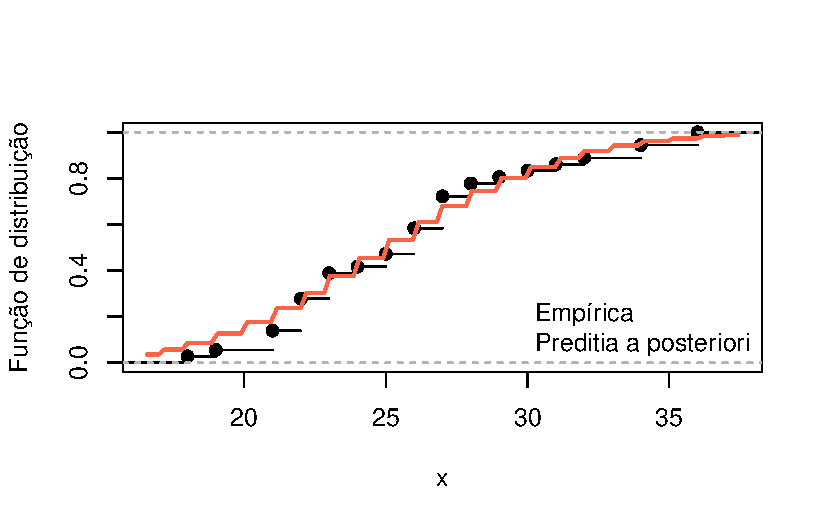
\includegraphics{poisson_files/figure-pdf/unnamed-chunk-3-1.pdf}

\section{O modelo Poisson para taxas}\label{o-modelo-poisson-para-taxas}

A taxa é o cociente entre o número de casos de um evento em determinado
intervalo de tempo e a população em risco, definida em um espaço e no
mesmo intervalo de tempo ``pessoas-tempo''. Note que, pela definição, a
taxa é uma estatística.

Seja \(N\) o tamanho da população no espaço/tempo e seja \(y\) o número
de casos do evento de interesse. Então,

\[\hbox{taxa} = \frac{y}{N}\]

Contudo, como \(N\) tende a ser muito maior que \(y\), é comum reportar
a taxa vezes \(10^k\), para algum \(k>0\).

Exemplo: Segundo o Anuário de Segurança Pública 2022, em 2021 houveram
68.885 casos de estupro. Considerando uma população de 212,7 milhões de
habitantes, a taxa de estupro para aquele ano foi de
\[\frac{68.885}{212.700.000}=3,23\times 10^{-4}\] casos por pessoa-ano.

Multiplicando a taxa por \(10^5\), temos uma taxa de 32,3 casos para
cada 100.000 habitantes.

Agora,considere que \(\lambda\) é o parâmetro taxa (ou seja, caso por
\(10^k\) pessoas). Então,

\[\hat{\lambda}=\frac{y}{N}\] é a estimativa para \(\lambda\). Como
\(y\) é uma contagem, é razoável supor que
\[\lambda =\frac{1}{N}E(Y|\lambda),\] e um modelo com essa
parametrização seria \(y|\lambda\sim\hbox{Poisson}(\lambda n)\).

Agora, considere que a população está particionada em \(m\) localidades.
Para um dado intervalo de tempo, sejam \(N_i\) e \(y_i\) a população da
localidade \(i\) e seu respectivo número de casos observados. Suponha
ainda que a taxa \(\lambda\) é comum para a população e que \(y_i\) e
\(y_j\) são independentes dado \(\lambda\). Assumindo a distribuição
Poisson, teremos

\[L(\lambda)=\prod_{i=1}^m\frac{e^{-\lambda n_i}(\lambda N_i)^{y_i}}{y_i!}\varpropto \lambda^{\sum_{i=1}^m y_i}e^{-\lambda \sum_{i=1}^m N_i}=\lambda^{\sum_{i=1}^n y_i}e^{-\lambda N},\]
onde \(N=\sum_{i=1}^m N_i\) é o tamanho da população. Como a
verossimilhança pertence à família exponencial, temos que o modelo
Gama\((r,s)\) é conjugado gerando a posteriori

\[\lambda|\mathbf{y}\sim\hbox{Gama}\left(\sum_{i=1}^{m}y_i+r,N+s\right)\equiv \hbox{Gamma}(r_1,s_1).\]

Considere agora um novo valor observado da localidade \(i\). Sua
preditiva a posteriori é dada por

\[\begin{align}
f(y^*_i|\boldsymbol{y})&=\int_0^\infty f(y^*_i|\lambda)f(\lambda|\boldsymbol{y})d\lambda\\
&\int_0^\infty \frac{e^{-\lambda N_i}(\lambda N_i)^{y_i^*}}{y_i^*!}\frac{s_1^{r_1}}{\Gamma(r_1)}\lambda^{r_1-1}e^{-\lambda s_1}d\lambda\\
&=\frac{\Gamma(r_1+y_i^*)}{y_i^*!\Gamma(r_1)}\left(\frac{s_i}{N_i+s_i}\right)^{r_1}\left(1-\frac{s_i}{N_i+s_i}\right)^{y_i^*},
\end{align}\] ou seja,
\[y_i^*|\boldsymbol{y}\sim\text{Binomial Negativa}\left(r_1,\frac{s_1}{N_i+s_1}\right),\]
cujo valor esperado é \[E(y_i^*|\boldsymbol{y})=\frac{r_1}{s_1}N_i.\]
Observe que \(y_1^*\) e \(y_j^*\) possuem a mesma distribuição somente
se \(N_i=N_j\).

\phantomsection\label{exm}
\begin{longtable}[]{@{}ll@{}}
\toprule\noalign{}
Unidade Federativa & População Estimada (1º de Julho de 2024) \\
\midrule\noalign{}
\endhead
\bottomrule\noalign{}
\endlastfoot
São Paulo & 45.973.194 \\
Minas Gerais & 21.322.691 \\
Rio de Janeiro & 17.219.679 \\
Bahia & 14.850.513 \\
Paraná & 11.824.665 \\
Rio Grande do Sul & 11.229.915 \\
Pernambuco & 9.539.029 \\
Ceará & 9.233.656 \\
Pará & 8.664.306 \\
Santa Catarina & 8.058.441 \\
Goiás & 7.350.483 \\
Maranhão & 7.010.960 \\
Amazonas & 4.281.209 \\
Paraíba & 4.145.040 \\
Espírito Santo & 4.102.129 \\
Mato Grosso & 3.836.399 \\
Rio Grande do Norte & 3.446.071 \\
Piauí & 3.375.646 \\
Alagoas & 3.220.104 \\
Distrito Federal & \\
Mato Grosso do Sul & 2.901.895 \\
Sergipe & 2.291.077 \\
Rondônia & 1.746.227 \\
Tocantins & 1.577.342 \\
Acre & 880.631 \\
Amapá & 802.837 \\
Roraima & 716.793 \\
\end{longtable}

\phantomsection\label{exm}
\textbf{Crime de estupro de vulnerável no interior do Amazonas}

Os dados a seguir foram cedidos pelo Observatório de Violência de Gênero
no Amazonas e compreendem os anos entre 2010 e 2012. A população em
risco é o número de mulheres co menos de 14 anos.

\begin{longtable}[]{@{}lll@{}}
\toprule\noalign{}
Cidade & Vítimas & Populacao feminina \\
\midrule\noalign{}
\endhead
\bottomrule\noalign{}
\endlastfoot
Amatura & 3 & 639 \\
Atalaia do Norte & 6 & 905 \\
Barreirinha & 12 & 1899 \\
Benjamin Constant & 2 & 2036 \\
Boa Vista do Ramos & 6 & 1060 \\
Fonte Boa & 0 & 1438 \\
Jutai & 1 & 1143 \\
Maues & 13 & 3421 \\
Nhamunda & 9 & 1168 \\
Parintins & 20 & 6700 \\
Santo Antonio do Ica & 7 & 1608 \\
Sao Paulo de Olivenca & 5 & 2033 \\
Tabatinga & 8 & 3095 \\
Tonantins & 1 & 1186 \\
\end{longtable}

Abaixo, organizamos os dados. A população é dividida por \(10^5\) para
que a taxa seja interpretada como número de casos para cada 100.000
mulheres menores de 14 anos.

\begin{Shaded}
\begin{Highlighting}[]
\CommentTok{\# banco de dados}
\NormalTok{casos }\OtherTok{\textless{}{-}} \FunctionTok{c}\NormalTok{( }\DecValTok{3}\NormalTok{, }\DecValTok{6}\NormalTok{, }\DecValTok{12}\NormalTok{, }\DecValTok{2}\NormalTok{, }\DecValTok{6}\NormalTok{, }\DecValTok{0}\NormalTok{, }\DecValTok{1}\NormalTok{, }\DecValTok{13}\NormalTok{, }\DecValTok{9}\NormalTok{, }\DecValTok{20}\NormalTok{, }\DecValTok{7}\NormalTok{, }\DecValTok{5}\NormalTok{, }\DecValTok{8}\NormalTok{, }\DecValTok{1}\NormalTok{ )   }

\NormalTok{pop }\OtherTok{\textless{}{-}} \FunctionTok{c}\NormalTok{(}\DecValTok{639}\NormalTok{, }\DecValTok{905}\NormalTok{, }\DecValTok{1899}\NormalTok{, }\DecValTok{2036}\NormalTok{, }\DecValTok{1060}\NormalTok{, }\DecValTok{1438}\NormalTok{, }\DecValTok{1143}\NormalTok{, }\DecValTok{3421}\NormalTok{, }\DecValTok{1168}\NormalTok{, }\DecValTok{6700}\NormalTok{, }\DecValTok{1608}\NormalTok{, }\DecValTok{2033}\NormalTok{, }\DecValTok{3095}\NormalTok{, }\DecValTok{1186}\NormalTok{)}
\NormalTok{pop }\OtherTok{\textless{}{-}}\NormalTok{ pop}\SpecialCharTok{/}\DecValTok{10}\SpecialCharTok{\^{}}\DecValTok{5}

\NormalTok{municipios }\OtherTok{\textless{}{-}} \FunctionTok{c}\NormalTok{( }\StringTok{\textquotesingle{}Amaturá\textquotesingle{}}\NormalTok{, }\StringTok{\textquotesingle{}Ataláia do Norte\textquotesingle{}}\NormalTok{, }\StringTok{\textquotesingle{}Barreirinha\textquotesingle{}}\NormalTok{, }\StringTok{\textquotesingle{}Benjamin Constant\textquotesingle{}}\NormalTok{,}\StringTok{\textquotesingle{}Boa Vista do Ramos\textquotesingle{}}\NormalTok{, }\StringTok{\textquotesingle{}Fonte Boa\textquotesingle{}}\NormalTok{, }\StringTok{\textquotesingle{}Jutaí\textquotesingle{}}\NormalTok{, }\StringTok{\textquotesingle{}Maués\textquotesingle{}}\NormalTok{, }\StringTok{\textquotesingle{}Nhamunda\textquotesingle{}}\NormalTok{, }\StringTok{\textquotesingle{}Parintins\textquotesingle{}}\NormalTok{, }\StringTok{\textquotesingle{}Sto Antônio do Iça\textquotesingle{}}\NormalTok{, }\StringTok{\textquotesingle{}São Paulo de Olivença\textquotesingle{}}\NormalTok{, }\StringTok{\textquotesingle{}Tabatinga\textquotesingle{}}\NormalTok{,}\StringTok{\textquotesingle{}Tonantins\textquotesingle{}}\NormalTok{)}
\end{Highlighting}
\end{Shaded}

A veromissilhança é dada por
\[L(\lambda)\propto \lambda^{93}e^{-0,28331\lambda }.\] Utilizando a
priori \(\lambda\sim\hbox{Gama}(.5,.00001)\), teremos a posteriori
\(\lambda\sim\hbox{Gama}(93.5,0.28332)\)

Vamos calcular o número de casos esperado segundo a preditiva a
posteriori para cada município.

\begin{Shaded}
\begin{Highlighting}[]
\NormalTok{r }\OtherTok{\textless{}{-}}\NormalTok{ .}\DecValTok{5}
\NormalTok{s }\OtherTok{\textless{}{-}}\NormalTok{ .}\DecValTok{00001}

\NormalTok{r1 }\OtherTok{\textless{}{-}} \FunctionTok{sum}\NormalTok{(casos) }\SpecialCharTok{+}\NormalTok{ r}
\NormalTok{s1 }\OtherTok{\textless{}{-}} \FunctionTok{sum}\NormalTok{(pop) }\SpecialCharTok{+}\NormalTok{ s}

\NormalTok{esperado }\OtherTok{\textless{}{-}}\NormalTok{ r1 }\SpecialCharTok{*}\NormalTok{ pop }\SpecialCharTok{/}\NormalTok{ s1}
\end{Highlighting}
\end{Shaded}

O gráfico abaixo apresenta o valor da média da preditiva a posteriori
contra o número de casos observados. Como esperado, os pares ordenados
flutuam em torno da linha \(y=x\).

\begin{Shaded}
\begin{Highlighting}[]
\FunctionTok{plot}\NormalTok{(casos, esperado, }\AttributeTok{xlab =} \StringTok{\textquotesingle{}Casos observados\textquotesingle{}}\NormalTok{, }\AttributeTok{ylab =} \StringTok{\textquotesingle{}Casos esperados\textquotesingle{}}\NormalTok{)}
\FunctionTok{abline}\NormalTok{(}\DecValTok{0}\NormalTok{,}\DecValTok{1}\NormalTok{,}\AttributeTok{lty =} \DecValTok{2}\NormalTok{)}
\end{Highlighting}
\end{Shaded}

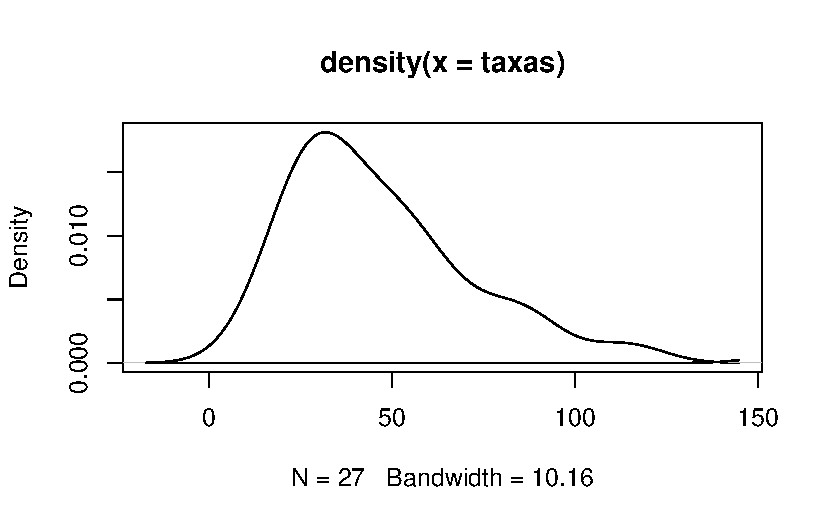
\includegraphics{poisson_files/figure-pdf/unnamed-chunk-6-1.pdf}

Mesmo que os pontos no gráfico acima estejam flutuando em torno da reta
\(y=x\), é importante determinar se sua distância até a reta é razoável.
Podemos construir intervalos de 95\% (de predição) para \(y^*_i\)
utilizando os quantis da preditiva a posteriori, ou seja, encontrando
\(q_1\) e \(q_2\) tais que \[\begin{align}
P(Y_i^*\leq q_1|\boldsymbol{y})&=0,025\\
P(Y_i^*\leq q_2|\boldsymbol{y})&=0,975.
\end{align}
\]

Observe ainda que
\[0,95\approx P(q_1\leq Y_i^*\leq q_2|\boldsymbol{y})=P\left(\frac{q_1}{N_i}\leq \frac{Y_i^*}{N_i}\leq \frac{q_2}{N_i}|\boldsymbol{y}\right),\]
o que implica que \((q_1,q_2)/N_i\) é um intervalo para taxa esperada.
Abaixo construímos os intervalos de 95\% (de predição) e colocamos o
número de casos observados.

\begin{Shaded}
\begin{Highlighting}[]
\CommentTok{\# limites do intervalo}
\NormalTok{lim\_inf }\OtherTok{\textless{}{-}} \FunctionTok{qnbinom}\NormalTok{(.}\DecValTok{025}\NormalTok{, }\AttributeTok{size =}\NormalTok{ r1, }\AttributeTok{prob =}\NormalTok{ s1}\SpecialCharTok{/}\NormalTok{(pop}\SpecialCharTok{+}\NormalTok{s1))}

\NormalTok{lim\_sup }\OtherTok{\textless{}{-}} \FunctionTok{qnbinom}\NormalTok{(.}\DecValTok{975}\NormalTok{, }\AttributeTok{size =}\NormalTok{ r1, }\AttributeTok{prob =}\NormalTok{ s1}\SpecialCharTok{/}\NormalTok{(pop}\SpecialCharTok{+}\NormalTok{s1))}

\CommentTok{\# gráfico}
\FunctionTok{plot.new}\NormalTok{()}
\FunctionTok{plot.window}\NormalTok{( }\AttributeTok{xlim =} \FunctionTok{c}\NormalTok{(}\SpecialCharTok{{-}}\DecValTok{500}\NormalTok{,}\DecValTok{1000}\NormalTok{), }\AttributeTok{ylim=}\FunctionTok{c}\NormalTok{(}\DecValTok{0}\NormalTok{,}\DecValTok{15}\NormalTok{))}
\FunctionTok{segments}\NormalTok{(lim\_inf}\SpecialCharTok{/}\NormalTok{pop,}\DecValTok{1}\SpecialCharTok{:}\DecValTok{14}\NormalTok{,lim\_sup}\SpecialCharTok{/}\NormalTok{pop,}\DecValTok{1}\SpecialCharTok{:}\DecValTok{14}\NormalTok{, }\AttributeTok{lwd =} \DecValTok{2}\NormalTok{)}
\FunctionTok{text}\NormalTok{(}\SpecialCharTok{{-}}\DecValTok{500}\NormalTok{,}\DecValTok{1}\SpecialCharTok{:}\DecValTok{14}\NormalTok{, municipios, }\AttributeTok{adj =}\DecValTok{0}\NormalTok{ )}
\FunctionTok{points}\NormalTok{(casos}\SpecialCharTok{/}\NormalTok{pop, }\DecValTok{1}\SpecialCharTok{:}\DecValTok{14}\NormalTok{, }\AttributeTok{pch =} \DecValTok{22}\NormalTok{, }\AttributeTok{cex =}\NormalTok{.}\DecValTok{9}\NormalTok{, }\AttributeTok{bg =} \StringTok{\textquotesingle{}red\textquotesingle{}}\NormalTok{)}
\end{Highlighting}
\end{Shaded}

\includegraphics{poisson_files/figure-pdf/unnamed-chunk-7-1.pdf}

Alguns municípios, como Nanhunda, foram substimados, enquanto outros,
como Fonte Boa, foram superestimados. Para estes 14 intervalos, é
esperado que \(14\times 0,05=0,7\) deles não cubram \(y_i\), o que não
está ocorrendo. Portanto, considerar que todos os municípios possuem a
mesma taxa pode ser um equívoco.

\section{Exercícios}\label{exercuxedcios-2}

\subsection{Mortes por coice de
cavalo}\label{mortes-por-coice-de-cavalo}

Ladislaus Bortkiewicz é o responsável pela popularização da distribuição
Poisson. Em seu livro intitulado A Lei dos Pequenos Números, é
apresentado um conjunto de dados no qual foi rastreado o número de
mortes por coice de cavalo em 14 corpos do exército prussiano ao longo
de 20 anos (de 1875 a 1894).

\begin{longtable}[]{@{}lllll@{}}
\toprule\noalign{}
Mortes por corpo \(\times\) ano & 0 & 1 & 2 & 3 \\
\midrule\noalign{}
\endhead
\bottomrule\noalign{}
\endlastfoot
109 & 65 & 22 & 3 & 1 \\
\end{longtable}

Determine se a distribuição Poisson é adequada para este conjunto de
dados. Em caso afirmativo, estime a taxa e dê um intervalo de
credibilidade de 95\%.

\subsection{Suicídios no Amazonas considerando capital e
interior}\label{suicuxeddios-no-amazonas-considerando-capital-e-interior}

O Amazonas possui uma característica peculiar: aproximadamente 50\% da
população vive na capital. Vimos anteriormente que o número de
suicídios, considerando os anos entre 2021 e 2023, podem ser modelados
por uma Poisson. A tabela abaixo divide esses dados entre capital e
interior.

\begin{longtable}[]{@{}lllll@{}}
\caption{Número de suicídios divididos entre capital e
interior}\tabularnewline
\toprule\noalign{}
Ano & 2021 & 2022 & 2023 & Total \\
\midrule\noalign{}
\endfirsthead
\toprule\noalign{}
Ano & 2021 & 2022 & 2023 & Total \\
\midrule\noalign{}
\endhead
\bottomrule\noalign{}
\endlastfoot
Capital & 133 & 124 & 138 & 395 \\
Interior & 164 & 173 & 201 & 538 \\
\end{longtable}

Determine se há evidências de que essas taxas são diferentes.

\bookmarksetup{startatroot}

\chapter{O modelo normal}\label{o-modelo-normal}

\section{A distribuição
normal-gama}\label{a-distribuiuxe7uxe3o-normal-gama}

Dizemos que \((X,Y)\sim NG(\mu,n_0,\nu,d^2)\) (lê-se normal-gama) se sua
função densidade conjunta é dada por

\[f(x,y)\propto y^{\frac{\nu+1}{2}-1}\exp\left\{-\frac{y}{2}n_0\left[(x-\mu)^2 + d^2\right]\right\}\]

onde \(\mu,x\in\mathbb{R}\) e \(d,y,c\in\mathbb{R}_+\). Colocando os
termos que não dependem de \(x\) junto com a constante de
proporcionalidade, podemos mostrar que

\[f(x|y)\propto \exp\left\{-\frac{y}{2}n_0(x-\mu)^2\right\}\] ou seja,
\(X|y\sim\hbox{Normal}(\mu,y^{-1}/n_0)\). Além disso, integrando
\(f(x,y)\) em \(x\), mostramos que

\[f(y)\propto y^{\frac{\nu+1}{2}-1}e^{-\frac{yn_0d^2}{2}}\int_{\mathbb{R}}\exp\left\{-\frac{y}{2}\left[n_0(x-\mu)^2\right]\right\}d\mu\propto y^{\frac{\nu}{2}-1}e^{-\frac{n_0d^2}{2}y}\]
ou seja, \(Y\sim\hbox{Gama}(\nu/2, n_0d^2/2)\). Por último, integrando
\(f(x,y)\) em \(y\) teremos

\[\begin{align}f(x)&\propto \int_0^\infty y^{\frac{\nu+1}{2}-1}\exp\left\{-\frac{y}{2}n_0\left[(x-\mu)^2 + d^2\right]\right\}dy \\&\propto \Gamma\left(\frac{\nu+1}{2}\right)\left\{1+\frac{\nu}{d^2}\frac{(x-\mu)^2}{\nu}\right\}^{-\frac{\nu+1}{2}}\end{align}\]
ou seja, \(X\sim t_{\nu}(\mu, d^2/\nu)\). Em especial, se \(\nu>1\)
então \(E(X)=\mu\) e, se \(\nu>2\) teremos que
\[Var(X)=\frac{d^2}{\nu-2}\]

\section{A função de
verossimilhança}\label{a-funuxe7uxe3o-de-verossimilhanuxe7a-1}

Seja \(X_1,\ldots,X_n\) uma amostra aleatória do modelo
\(X|\mu,\phi\sim\hbox{Normal}(\mu,\phi^{-1})\), onde \(\phi\),
denominado precisão, é o inverso da variância. A função de
verossimilhança deste modelo pode ser escrita como

\[L(\mu,\phi)\propto \phi^{\frac{n}{2}}\exp\left\{-\frac{n\phi}{2}(\bar{x}-\mu)^2 -\frac{ns^2\phi}{2}\right\}\]
onde \[s^2=\frac{1}{n}\sum_{i=1}^n(x_i-\bar{x})^2\] é a estimativa de
máxima verossimilhança para \(\phi^{-1}\).

\section{Posteriori com prioris
impróprias}\label{posteriori-com-prioris-impruxf3prias}

Considerando as prioris impróprias \(\pi(\phi)\propto \phi^{-1}\),
\(\pi(\mu)\propto 1\) e que \(\pi(\mu,\phi)=\pi(\mu)\pi(\phi)\), teremos
que

\[\pi(\mu,\phi|\boldsymbol{x})\propto \phi^{\frac{n}{2}-1}\left\{-\frac{\phi}{2}n\left[ (\bar{x}-\mu)^2 +s^2\right]\right\}\]
ou seja, \(\mu,\phi|\boldsymbol{x}\sim\hbox{NG}(\bar{x},n,n-1,s^2)\), o
que implica em:

\[\begin{align}
\mu|\phi,\boldsymbol{x}&\sim\hbox{Normal}\left(\bar{x},\frac{\phi^{-1}}{n}\right)\\
\phi|\boldsymbol{x}&\sim\hbox{Gama}\left(\frac{n-1}{2},\frac{ns^2}{2}\right)\\
\mu|\boldsymbol{x}&\sim t_{n-1}\left(\bar{x},\frac{s^2}{n-1}\right)
\end{align}\]

Disto, teremos que

\begin{longtable}[]{@{}lll@{}}
\toprule\noalign{}
Parâmetro & Estimativa & Erro \\
\midrule\noalign{}
\endhead
\bottomrule\noalign{}
\endlastfoot
\(\mu\) & \(\bar{x}\) & \(\frac{s}{\sqrt{n-3}}\) \\
\(\phi\) & \(\frac{n-1}{ns^2}\) & \(\frac{\sqrt{2(n-1)}}{s^2n}\) \\
\end{longtable}

\section{Posteriori com a priori de
Jeffreys}\label{posteriori-com-a-priori-de-jeffreys}

O logaritmo da função de verossimilhança é

\[l(\mu,\phi)=\frac{n}{2}\log\phi -\frac{n}{2}\phi\left[(\bar{x}-\mu)^2 + s^2\right]\]

As derivadas de primeira ordem em \(\mu\) e \(\phi\) são \[\begin{align}
\frac{\partial}{\partial \mu}l(\mu,\phi)&=n\phi(\bar{x}-\mu)\\
\frac{\partial}{\partial \phi}l(\mu,\phi)&=\frac{n}{2\phi}-\frac{n}{2}\left[(\bar{x}-\mu)^2 + s^2\right]\\
\end{align}\]

e as de segunda ordem são \[\begin{align}
\frac{\partial^2}{\partial \mu^2}l(\mu,\phi)&=-n\phi\\
\frac{\partial^2}{\partial \phi^2}l(\mu,\phi)&=-\frac{n}{2\phi^2}\\
\frac{\partial^2}{\partial \mu\partial \phi}l(\mu,\phi)&=0\\
\end{align}
\] logo, a matriz de informação de Fisher é
\[\mathcal{I}_n(\mu,\phi)=n\left[\begin{array}{cc}\phi & 0 \\0 & \frac{1}{2\phi^2}\end{array}\right],\]
e a priori de Jeffreys é
\[\pi(\mu,\phi)\propto \sqrt{|\mathcal{I}_n(\mu,\phi)|}=\phi^{-1/2},\]
que implica na posteriori

\[\pi(\mu,\phi|\boldsymbol{x})\propto \phi^{\frac{n+1}{2}-1}\left\{-\frac{n\phi}{2}\left[(\bar{x}-\mu)^2 +s^2 \right]\right\}\]
ou seja, \(\mu,\phi|\boldsymbol{x}\sim\hbox{NG}(\bar{x},n,n,s^2)\), o
que implica em:

\[\begin{align}
\mu|\phi,\boldsymbol{x}&\sim\hbox{Normal}\left(\bar{x},\frac{\phi^{-1}}{n}\right)\\
\phi|\boldsymbol{x}&\sim\hbox{Gama}\left(\frac{n}{2},\frac{ns^2}{2}\right)\\
\mu|\boldsymbol{x}&\sim t_{n}\left(\bar{x},\frac{s^2}{n}\right)
\end{align}\]

Disto, teremos que

\begin{longtable}[]{@{}lll@{}}
\toprule\noalign{}
Parâmetro & Estimativa & Erro \\
\midrule\noalign{}
\endhead
\bottomrule\noalign{}
\endlastfoot
\(\mu\) & \(\bar{x}\) & \(\frac{s}{\sqrt{n-2}}\) \\
\(\phi\) & \(\frac{1}{s^{2}}\) & \(\frac{\sqrt{2}}{s^2\sqrt{n}}\) \\
\end{longtable}

\section{Posteriori para a priori
conjugada}\label{posteriori-para-a-priori-conjugada}

Considere que \((\mu,\phi)\sim \hbox{NG}(m_0,n_0,\nu_0,s^2_0)\). Esta
priori é conjugada para o modelo normal, uma vez que

\[\begin{align}
\pi(\mu,\phi|\boldsymbol{x})&\propto \phi^{\frac{n}{2}}\exp\left\{-\frac{\phi}{2}n\left[(\bar{x}-\mu)^2+ s^2\right]\right\}\phi^{\frac{\nu_0+1}{2}-1}\exp\left\{-\frac{\phi}{2}n_0\left[(\mu-m_0)^2 + s_0^2\right]\right\}\\
&\phi^{\frac{\nu_0+n}{2}-1}\exp\left\{-\frac{\phi}{2}\left[n(\bar{x}-\mu)^2 + n_0(\mu-m_0)^2+ns^2 + n_0s^2_0\right]\right\}\end{align}.\]
Como
\[n(\bar{x}-\mu)^2 +n_0(\mu-m_0)^2 = (n+n_0)(\mu-m_1)^2+\frac{n n_0}{n+n_0}(\bar{x}-m_0)^2\]
onde \[\begin{align}
m_1&=\frac{n}{n+n_0}\bar{x}+\frac{n_0}{n+n_0}m_0
\end{align},\] teremos \[\begin{align}
\pi(\mu,\phi|\boldsymbol{x})&\propto \phi^{\frac{\nu_1+1}{2}-1}\exp\left\{-\frac{\phi}{2}n_1\left[(\mu-m_1)^2 + d_1^2\right]\right\}\end{align},\]
onde \[\begin{align}
\nu_1&=\nu_0+n\\
n_1&=n_0+n\\
m_1&=\frac{n}{n1}\bar{x}+\frac{n_0}{n_1}m_0\\
d_1^2& = \frac{n_0n}{n_1^2}(\bar{x}-m_0)^2+\frac{n}{n_1}s^2 + \frac{n_0}{n_1}s^2_0
\end{align}\] ou seja,
\(\mu,\phi|\boldsymbol{x}\sim\hbox{NG}(m_1,n+n_0,\nu_0+n,d_1^2)\), o que
implica em:

\[\begin{align}
\mu|\phi,\boldsymbol{x}&\sim\hbox{Normal}\left(m_1,\frac{\phi^{-1}}{n+n_0}\right)\\
\phi|\boldsymbol{x}&\sim\hbox{Gama}\left(\frac{n+\nu_0}{2},\frac{(n+n_0)d_1^2}{2}\right)\\
\mu|\boldsymbol{x}&\sim t_{n}\left(m_1,\frac{d^2_1}{\nu_0+n}\right)
\end{align}\]

Disto, teremos que

\begin{longtable}[]{@{}
  >{\raggedright\arraybackslash}p{(\columnwidth - 4\tabcolsep) * \real{0.3472}}
  >{\raggedright\arraybackslash}p{(\columnwidth - 4\tabcolsep) * \real{0.4028}}
  >{\raggedright\arraybackslash}p{(\columnwidth - 4\tabcolsep) * \real{0.2500}}@{}}
\toprule\noalign{}
\begin{minipage}[b]{\linewidth}\raggedright
Parâmetro
\end{minipage} & \begin{minipage}[b]{\linewidth}\raggedright
Estimativa
\end{minipage} & \begin{minipage}[b]{\linewidth}\raggedright
Erro
\end{minipage} \\
\midrule\noalign{}
\endhead
\bottomrule\noalign{}
\endlastfoot
\(\mu\) & \(\frac{n}{n+n_0}\bar{x}+\frac{n_0}{n+n_0}m_0\) &
\(\frac{d_1}{\sqrt{n+\nu_0-2}}\) \\
\(\phi\) & \(\frac{n+\nu_0}{(n+n_0)d_1^2}\) &
\(\frac{\sqrt{2(n+\nu_0)}}{d_1^2(n+n_0)}\) \\
\end{longtable}

\section{Detecção de outliers}\label{detecuxe7uxe3o-de-outliers}

\bookmarksetup{startatroot}

\chapter{Binomial negativa}\label{binomial-negativa}

\section{O modelo binomial negativo}\label{o-modelo-binomial-negativo}

A distribuição Poisson é muito comum em problemas de contagem. Como sua
esperança e variância são iguais, o termo sobredispersão foi cunhado na
literatura como uma variância maior que a média, o que seria indício de
que o modelo Poisson não é adequado (de modo análogo, há o conceito de
subdispersão, mas não é um fenômeno comum).

Dizemos que \(X|\rho,\phi\sim\hbox{Binomial Negativa}\) se

\[p(x|\rho,\phi)=\frac{\Gamma(\phi+x)}{x!\Gamma(\phi)}\rho^\phi(1-\rho)^x,\]
onde \(x\in\mathbb{N}\), \(\rho\in(0,1)\) e \(\phi>0\).

Existem diversos motivos para considerar o modelo binomial negativo uma
alternativa quando o modelo Poisson não parece ser adequado. Primeiro,
temos que \(E(X|\rho,\phi)=\phi(1-\rho)/\rho\) e
\(Var(X|\rho,\phi)=E(X|\rho,\phi)/\rho\), logo, a sobredispersão está
presente no modelo. Além disso, se
\(X|\lambda\sim\hbox{Poisson}(\lambda)\) e
\(\lambda\sim\hbox{Gama}(\phi, \rho/(1-\rho))\), então
\(X|\phi,\rho\sim\hbox{Binomial Negativa}(\phi,\rho)\) logo, este modelo
é uma mistura do modelo Poisson. Por último, fazendo
\[\mu=\phi\frac{1-\rho}{\rho}\Rightarrow \rho(\phi)=\frac{\phi}{\phi+\mu},\]
pode-de mostrar que
\[\lim_{\phi\rightarrow\infty}p(x|\phi)=\frac{e^{-\mu}\mu^x}{x!}\] ou
seja, o modelo Poisson também pode ser vist como um caso limite do
binomial negativo.

\section{\texorpdfstring{Priori para \(\phi\)
condicionado}{Priori para \textbackslash phi condicionado}}\label{priori-para-phi-condicionado}

Quando \(\phi\) é conhecido, a verossimilhança do modelo se torna

\[L(\rho|\phi)\propto \rho^{n\phi}(1-\rho)^{\sum_{i=1}^n x_i},\] logo, o
modelo Beta\((a,b)\) é conjugado, com a posteriori dada por
\[\rho|\boldsymbol{x},\phi\sim\hbox{Beta}\left(n\phi+a,\sum_{i=1}^n x_i+b\right).\]

A priori de Jeffreys é dada por

\[\pi(\rho)\propto \frac{1}{\rho(1-\rho)^{1/2}},\] o que implica na
posteriori
\[\rho|\boldsymbol{x},\phi\sim\hbox{Beta}\left(n\phi,\sum_{i=1}^n x_i+\frac{1}{2}\right).\]

\section{\texorpdfstring{Priori para
\(\phi\)}{Priori para \textbackslash phi}}\label{priori-para-phi}

Seja \(\pi(\phi)\pi(\rho)\) a priori para \((\phi,\rho)\). Então,
teremos que

\[\pi(\phi,\rho|\boldsymbol{x})\propto \frac{\prod_{i=1}^n\Gamma(\phi+x_i)}{\Gamma(\phi)^n}\rho^{n\phi}(1-\rho)^{\sum_{i=1}^n x_i}\pi(\phi)\pi(\rho).\]

Assumindo qualquer uma das prioris da seção anterior, teremos

\[\pi(\phi,\rho|\boldsymbol{x})\propto \frac{\prod_{i=1}^n\Gamma(\phi+x_i)}{\Gamma(\phi)^n}B\left(a_0+n\phi,b_0+\sum_{i=1}^nx_i\right)\pi(\phi)\pi(\rho|\phi,\boldsymbol{x}),\]

logo,

\[\pi(\phi|\boldsymbol{x})\propto \frac{\prod_{i=1}^n\Gamma(\phi+x_i)}{\Gamma(\phi)^n}B\left(a_0+n\phi,b_0+\sum_{i=1}^nx_i\right)\pi(\phi)\]

Como a posteriori de \(\phi\) não é uma distribuição conhecida,
precisamos construir um simulador. O algoritmo Metropolis-Hastings é uma
boa escolha, uma vez que a constante de proporcionalidade da densidade é
desconhecida.

Algoritmo Metropolis-Hastings

O Metropolis-Hastings simula se utiliza de uma distribuição que sabemos
simular (denominada proposta) para gerar uma cadeia de Markov cuja
distribuição estacionária é a distribuição de interesse.

Na \(j\)-ésima itereção, a simulação do valor proposto \(\phi^*\) é
baseada no valor atual da cadeia, \(\phi^{(j-1)}\). Como \(\phi>0\), a
proposta \(\phi^*\sim \hbox{Gamma}(\tau\phi^{(j-1)},\tau)\) é adequada
uma vez que \[E(\phi^*)=\phi^{(j-1)}\] e
\[\sqrt{Var(\phi^*)}=\frac{\phi^{(j-1)}}{\tau}\] Acima, \(\tau\) é
denominado \emph{tunning} (afinação em tradução livre) e deve ser
escolhido para que a cadeia tenha o número de aceites da proposta
controlado (algo em torno de 23\% ).

Abaixo, segue o algoritmo

\begin{enumerate}
\def\labelenumi{\arabic{enumi}.}
\item
  Faça \(j=0\) e escolha um valor para \(\phi^{(0)}\) (a estimativa de
  máxima verossimilhança, por exemplo). Faça um contador de aceites,
  começando com \(k=0\).
\item
  Para o passo \(j\):
\end{enumerate}

\begin{itemize}
\tightlist
\item
  Simule \(\phi^*\sim\hbox{Gama}(\tau\phi^{j-1},\tau)\)
\item
  Calcule
\end{itemize}

\[prob = \frac{\pi(\phi^*|\boldsymbol{x})}{\pi(\phi^{(j-1)}|\boldsymbol{x})}\frac{g(\phi^{(j-1)}|\tau\phi^*,\tau)}{g(\phi^*|\tau\phi^{(j-1)},\tau)},\]
onde \(g(.|a,b)\) é a função densidade do modelo gama. + Simule
\(u\sim\hbox{Uniforme}(0,1)\). Se \(u<prob\), faça \(\phi^{(j)}=\phi^*\)
e \(k=k+1\) (houve um aceite). Senão, faça \(\phi^{(j)}=\phi^{(j-1)}\).

\bookmarksetup{startatroot}

\chapter{Aproximação normal e seu uso com o
Metropolis-Hastings}\label{aproximauxe7uxe3o-normal-e-seu-uso-com-o-metropolis-hastings}

\section{Aproximação da posteriori pela distribuição
normal}\label{aproximauxe7uxe3o-da-posteriori-pela-distribuiuxe7uxe3o-normal}

Assuma que \(\boldsymbol{\theta}\in\mathbb{R}^q\). Seja
\(\ell(\boldsymbol{\theta})=\log L(\boldsymbol{\theta})\) a função
log-verossimilhança e \(\hat{\boldsymbol{\theta}}\) a estimativa de
máxima verossimilhaça para \(\boldsymbol{\theta}\). Considere a seguinte
aproximação de \(\ell(\boldsymbol{\theta})\) em séries de Taylor

\[\ell(\boldsymbol{\theta})\approx  \ell(\hat{\boldsymbol{\theta}})+\frac{1}{2}(\boldsymbol{\theta}-\hat{\boldsymbol{\theta}})'\mathcal{H}(\hat{\boldsymbol{\theta}})(\boldsymbol{\theta}-\hat{\boldsymbol{\theta}})\]
onde \(\boldsymbol{\theta}\) é a matriz hessiana (de derivadas segunda)
aplicada em \(\hat{\boldsymbol{\theta}}\). Deste modo, teremos que
\[\pi(\boldsymbol{\theta}|\boldsymbol{x})\propto \exp\left\{-\frac{1}{2}(\boldsymbol{\theta}-\hat{\boldsymbol{\theta}})'\left[-\mathcal{H}(\hat{\boldsymbol{\theta}})\right](\boldsymbol{\theta}-\hat{\boldsymbol{\theta}})\right\}\pi(\boldsymbol{\theta})\]

Utilizando a priori imprópria \(\pi(\boldsymbol{\theta})\), temos que
\(\boldsymbol{\theta}|\boldsymbol{x}\approx \hbox{Normal}(\hat{\boldsymbol{\theta}},-\mathcal{H}(\hat{\boldsymbol{\theta}})^{-1})\).

Note que as informações necessárias para a aproximação da posteriori
acima podem ser obtidas via função \texttt{optim}.

Exemplo A amostra abaixo foi simulada do modelo Gama\((\alpha,\beta)\)
(o valor dos parâmetros foram omitidos de propósito)

\begin{Shaded}
\begin{Highlighting}[]
\NormalTok{x}
\end{Highlighting}
\end{Shaded}

\begin{verbatim}
 [1] 0.2769550 1.1902521 1.1543901 0.6836040 1.2951363 0.8468467 0.7626888
 [8] 0.3830976 0.2270072 0.2785412 0.3853067 0.4818242 0.2021683 0.8914625
[15] 0.7718524 0.9455476 0.8702839 0.5309044 1.2858882 1.0415047
\end{verbatim}

Como \(\alpha,\beta>0\), considere que \(\alpha=\exp\{\theta_1\}\) e
\(\beta=\exp\{\theta_2\}\) (deste modo,
\(\boldsymbol{\theta}\in\mathbb{R}^2\)).

A função de log-verossimilhança deste modelo é

\begin{Shaded}
\begin{Highlighting}[]
\NormalTok{logveross }\OtherTok{\textless{}{-}} \ControlFlowTok{function}\NormalTok{(theta)\{ }\FunctionTok{sum}\NormalTok{(}\FunctionTok{dgamma}\NormalTok{(x, }\FunctionTok{exp}\NormalTok{(theta[}\DecValTok{1}\NormalTok{]), }\FunctionTok{exp}\NormalTok{(theta[}\DecValTok{2}\NormalTok{]), }\AttributeTok{log =}\NormalTok{ T))}
\NormalTok{\}}
\end{Highlighting}
\end{Shaded}

Podemos utilizar a função \texttt{optim} para obter as estimativas de
máxima verossimilhança e a matriz hessiana. Contudo, primeiro devemos
observar que esta função é um minimizador, logo, queremos que
\(\boldsymbol{\theta}\) que minimize \(-\ell({\boldsymbol{\theta}})\).

\begin{Shaded}
\begin{Highlighting}[]
\NormalTok{opt }\OtherTok{\textless{}{-}} \FunctionTok{optim}\NormalTok{( }\FunctionTok{c}\NormalTok{(}\DecValTok{0}\NormalTok{,}\DecValTok{0}\NormalTok{), }\ControlFlowTok{function}\NormalTok{(q) }\SpecialCharTok{{-}}\FunctionTok{logveross}\NormalTok{(q), }\AttributeTok{hessian =}\NormalTok{ T)}
\NormalTok{opt}
\end{Highlighting}
\end{Shaded}

\begin{verbatim}
$par
[1] 1.245897 1.567152

$value
[1] 7.435047

$counts
function gradient 
      65       NA 

$convergence
[1] 0

$message
NULL

$hessian
          [,1]      [,2]
[1,]  80.46195 -69.52104
[2,] -69.52104  69.52342
\end{verbatim}

No objeto \texttt{opt}, a lista \texttt{par} é o vetor com as
estimativas de máxima verossimilhança, enquanto que \texttt{hessian} é o
valor de \(-\mathcal{H}(\hat{\boldsymbol{\theta}})\).

A inversa de \texttt{opt\$hessian} vai dar a matriz de covariância entre
\(\theta_1\) e \(\theta_2\) a posteriori.

\begin{Shaded}
\begin{Highlighting}[]
\NormalTok{Sigma }\OtherTok{\textless{}{-}} \FunctionTok{solve}\NormalTok{(opt}\SpecialCharTok{$}\NormalTok{hessian)}
\NormalTok{Sigma}
\end{Highlighting}
\end{Shaded}

\begin{verbatim}
           [,1]       [,2]
[1,] 0.09138023 0.09137711
[2,] 0.09137711 0.10575762
\end{verbatim}

Agora, podemos simular \(\theta_1\) e \(\theta_2\) a posteriori:

\begin{Shaded}
\begin{Highlighting}[]
\FunctionTok{require}\NormalTok{(mvtnorm)}
\end{Highlighting}
\end{Shaded}

\begin{verbatim}
Carregando pacotes exigidos: mvtnorm
\end{verbatim}

\begin{verbatim}
Warning: pacote 'mvtnorm' foi compilado no R versão 4.4.3
\end{verbatim}

\begin{Shaded}
\begin{Highlighting}[]
\NormalTok{theta\_sim }\OtherTok{\textless{}{-}} \FunctionTok{rmvnorm}\NormalTok{(}\DecValTok{500}\NormalTok{, opt}\SpecialCharTok{$}\NormalTok{par, Sigma)}
\end{Highlighting}
\end{Shaded}

Por último, podemos fazer inferências sobre \(\alpha=\exp\{\theta_1\}\)
e \(\beta=\exp\{\theta_2\}\):

\begin{Shaded}
\begin{Highlighting}[]
\CommentTok{\# intervalos de credibilidade para alfa}
\FunctionTok{quantile}\NormalTok{(}\FunctionTok{exp}\NormalTok{(theta\_sim[,}\DecValTok{1}\NormalTok{]), }\FunctionTok{c}\NormalTok{(.}\DecValTok{025}\NormalTok{,.}\DecValTok{975}\NormalTok{))}
\end{Highlighting}
\end{Shaded}

\begin{verbatim}
    2.5%    97.5% 
1.978850 6.350455 
\end{verbatim}

\begin{Shaded}
\begin{Highlighting}[]
\CommentTok{\# intervalos de credibilidade para beta}
\FunctionTok{quantile}\NormalTok{(}\FunctionTok{exp}\NormalTok{(theta\_sim[,}\DecValTok{2}\NormalTok{]), }\FunctionTok{c}\NormalTok{(.}\DecValTok{025}\NormalTok{,.}\DecValTok{975}\NormalTok{))}
\end{Highlighting}
\end{Shaded}

\begin{verbatim}
    2.5%    97.5% 
2.582863 8.865732 
\end{verbatim}

\section{Metropolis revisitado}\label{metropolis-revisitado}

A diferença entre o algoritmo Metropolis e o Metropolis-Hastings está na
escolha da distribuição proposta. No primeiro, a proposta é simétrica,
\[g(x|y)=g(y|x).\] Com isso, teremos que
\[\frac{f(x)}{f(y)}\frac{g(y|x)}{g(x|y)}=\frac{f(x)}{f(y)}\] e a
probabilidade de aceitação da cadeia é baseada somente na distribuição
alvo \(f\).

No algoritmo Metropolis, é comum escolher a distribuição proposta como
sendo uma normal. Uma escolha razoável é utilizar como proposta
aproximação normal vista na seção anterior.

Exemplo Consideremos novamente a amostra do exemplo anterior. A função
de verossimilhança é
\[L(\theta)=\prod_{i=1}^n \frac{\beta(\theta_2)^{\alpha(\theta_1)}}{\Gamma(\alpha(\theta_1))} x_i^{\alpha(\theta_1)-1}e^{-\beta(\theta_2)x_i}\]
onde \(\alpha(\theta_1)=e^{\theta_1}\),
\(\beta(\theta_2)=e^{\theta_2}\). Além disso ,considere ad prioris
independentes \(\theta_i\sim\hbox{Normal}(0,100)\). Então, devemos
simular do modelo

\[\pi(\theta|\boldsymbol{x})\propto \left[\frac{\beta(\theta_2)^{\alpha(\theta_1)}}{\Gamma(\alpha(\theta_1))}\right]^n \left[\prod_{i=1}^n x_i\right]^{\alpha(\theta_1)}e^{-\beta(\theta_2)\sum_{i=1}^{n}x_i}e^{-\frac{1}{200}(\theta_1^2 + \theta_2^2)}\]

A posteriori aproximada, que encontramos no exemplo anterior é
\[\boldsymbol{\theta}|\boldsymbol{x}\approx N \left[ \left(\begin{array}{c}1,24\\1,56 \end{array}\right),\left(\begin{array}{cc}0,09 & 0,09\\0,09 &0,11\end{array}\right)\right]\]

Vamos aproveitar a estrutura de covariâncias acima para usar a proposta

\[\boldsymbol{\theta}^*|\boldsymbol{x}\sim N \left[ \boldsymbol{\theta}^{(j-1)},\tau\left(\begin{array}{cc}0,09 & 0,09\\0,09 &0,11\end{array}\right)\right]\]
onde \(\boldsymbol{\theta}^*\) é o candidato gerado e
\(\boldsymbol{\theta}^{(j)}\) é o estado atual da cadeia e \(\tau\) é o
\textbf{tunning} da cadeia.

\begin{Shaded}
\begin{Highlighting}[]
\NormalTok{B }\OtherTok{\textless{}{-}} \DecValTok{10000} \CommentTok{\# número de iterações}
\NormalTok{theta }\OtherTok{\textless{}{-}} \FunctionTok{array}\NormalTok{(}\ConstantTok{NA\_real\_}\NormalTok{, }\FunctionTok{c}\NormalTok{(B,}\DecValTok{2}\NormalTok{))}

\NormalTok{theta[}\DecValTok{1}\NormalTok{,] }\OtherTok{\textless{}{-}}\NormalTok{ opt}\SpecialCharTok{$}\NormalTok{par }\CommentTok{\# valor inicial da cadeia é a emv}
\NormalTok{tau }\OtherTok{\textless{}{-}} \DecValTok{1}             \CommentTok{\# tunning}
\NormalTok{cont }\OtherTok{\textless{}{-}} \DecValTok{0}            \CommentTok{\# contador de aceites}

\ControlFlowTok{for}\NormalTok{(j }\ControlFlowTok{in} \DecValTok{2}\SpecialCharTok{:}\NormalTok{B)\{}
  \CommentTok{\#simule um candidato}
\NormalTok{  theta\_cand }\OtherTok{\textless{}{-}} \FunctionTok{rmvnorm}\NormalTok{(}\DecValTok{1}\NormalTok{, theta[j}\DecValTok{{-}1}\NormalTok{,], tau}\SpecialCharTok{*}\NormalTok{Sigma)}
  
  \CommentTok{\# calcule a probabilidade do salto}
\NormalTok{  lnum }\OtherTok{\textless{}{-}} \FunctionTok{logveross}\NormalTok{(theta\_cand) }\SpecialCharTok{+}
    \FunctionTok{sum}\NormalTok{(}\FunctionTok{dnorm}\NormalTok{(theta\_cand[}\DecValTok{1}\NormalTok{,],}\DecValTok{0}\NormalTok{,}\DecValTok{10}\NormalTok{, }\AttributeTok{log =}\NormalTok{ T))}
  
\NormalTok{  lden }\OtherTok{\textless{}{-}} \FunctionTok{logveross}\NormalTok{(theta[j}\DecValTok{{-}1}\NormalTok{,]) }\SpecialCharTok{+}
    \FunctionTok{sum}\NormalTok{(}\FunctionTok{dnorm}\NormalTok{(theta[j}\DecValTok{{-}1}\NormalTok{,],}\DecValTok{0}\NormalTok{,}\DecValTok{10}\NormalTok{, }\AttributeTok{log =}\NormalTok{ T))}
  
\NormalTok{  prob }\OtherTok{\textless{}{-}} \FunctionTok{exp}\NormalTok{( lnum }\SpecialCharTok{{-}}\NormalTok{ lden)}
  
  \CommentTok{\# verifique o salto}
\NormalTok{  u }\OtherTok{\textless{}{-}} \FunctionTok{runif}\NormalTok{(}\DecValTok{1}\NormalTok{)}
  \ControlFlowTok{if}\NormalTok{( u }\SpecialCharTok{\textless{}}\NormalTok{ prob)\{}
\NormalTok{    theta[j, ] }\OtherTok{\textless{}{-}}\NormalTok{ theta\_cand}
\NormalTok{    cont }\OtherTok{\textless{}{-}}\NormalTok{ cont}\SpecialCharTok{+}\DecValTok{1}
\NormalTok{  \} }\ControlFlowTok{else}\NormalTok{ \{}
\NormalTok{    theta[j,] }\OtherTok{\textless{}{-}}\NormalTok{ theta[j}\DecValTok{{-}1}\NormalTok{,]}
\NormalTok{  \}}
\NormalTok{\}}

\NormalTok{cont}\SpecialCharTok{/}\NormalTok{B}
\end{Highlighting}
\end{Shaded}

\begin{verbatim}
[1] 0.5628
\end{verbatim}

\begin{Shaded}
\begin{Highlighting}[]
\NormalTok{theta\_sim }\OtherTok{\textless{}{-}}\NormalTok{ theta[ }\FunctionTok{seq}\NormalTok{(B}\SpecialCharTok{/}\DecValTok{2}\NormalTok{, B, }\DecValTok{15}\NormalTok{),]}
\FunctionTok{acf}\NormalTok{(theta\_sim)}
\end{Highlighting}
\end{Shaded}

\includegraphics{aproximacaoNormal_files/figure-pdf/unnamed-chunk-8-1.pdf}

Por fim, as estimativas intervalares para \((\alpha,\beta)\) são

\begin{Shaded}
\begin{Highlighting}[]
\FunctionTok{quantile}\NormalTok{(}\FunctionTok{exp}\NormalTok{(theta\_sim[,}\DecValTok{1}\NormalTok{]), }\FunctionTok{c}\NormalTok{(.}\DecValTok{025}\NormalTok{,.}\DecValTok{975}\NormalTok{))}
\end{Highlighting}
\end{Shaded}

\begin{verbatim}
    2.5%    97.5% 
1.699256 5.644593 
\end{verbatim}

\begin{Shaded}
\begin{Highlighting}[]
\CommentTok{\# intervalos de credibilidade para beta}
\FunctionTok{quantile}\NormalTok{(}\FunctionTok{exp}\NormalTok{(theta\_sim[,}\DecValTok{2}\NormalTok{]), }\FunctionTok{c}\NormalTok{(.}\DecValTok{025}\NormalTok{,.}\DecValTok{975}\NormalTok{))}
\end{Highlighting}
\end{Shaded}

\begin{verbatim}
    2.5%    97.5% 
2.087772 7.675778 
\end{verbatim}

\bookmarksetup{startatroot}

\chapter{Misturas de
distribuições}\label{misturas-de-distribuiuxe7uxf5es}

Dizemos que \(X\sim f(.)\) é uma mistura se existe uma variável \(Z\)
tal que

\[f(x)=\int f(x|z)f(z)dz.\]

A variável \(Z\) é denominada latente e a função \(f(x,z)\) é denominada
modelo aumentado.

Seja \((X_1,Z_1),\ldots,(X_n,Y_n)\) uma amostra aleatória do modelo
aumentado \(f(x,z|\theta)\) e seja \(\pi(\theta)\) a priori para
\(\theta\). Existem situações nas quais é mais fácil simular do modelo
\[\pi(\theta,\boldsymbol{z}|\boldsymbol{x})\varpropto f(\boldsymbol{x},\boldsymbol{z}|\theta)\pi(\theta).\]

A distribuição de \(\theta\) (ou \(\boldsymbol{Z}\)) dado as demais
variáveis do modelo é denominada condicional completa, que neste
problema são:

\[f(\boldsymbol{z}|\boldsymbol{x},\theta)\] e
\[\pi(\theta|\boldsymbol{z},\boldsymbol{x},\theta)\]

Em particular, se é fácil simular das condicionais completas, podemos
utilizar o Amostrador de Gibbs, que consiste no seguinte algoritmo:

Amostrador de Gibbs

Inicie a cadeia com fazendo \(j=0\) e escolhendo \(\theta^{(0)}\)

No \(j\)-ésimo passo:

\begin{enumerate}
\def\labelenumi{\arabic{enumi}.}
\item
  Simule
  \(\boldsymbol{z^{(j)}}\sim f(\boldsymbol{z}|\boldsymbol{x},\theta^{(j-1)})\)
\item
  Simule \(\theta^{(j)}\sim \pi(\theta|\boldsymbol{z},\boldsymbol{x})\)
\end{enumerate}

O Amostrador de Gibbs é uma cadeia de Markov cuja distribuição
estacionária é \(\pi(\theta,\boldsymbol{z}|\boldsymbol{x})\)

\section{Modelos com inflação de
zeros}\label{modelos-com-inflauxe7uxe3o-de-zeros}

Quando são observados mais zeros do que o esperado pelo modelo de
contagem assumido para a verossimilhança, é usual considerar um modelo
com inflação de zeros. Nesse tipo de modelo, assumimos que existe uma
variável \(Z|p\sim\hbox{Bernoulli}(\rho)\) tal que:

\[X=\left\{\begin{array}{ll}0, & \hbox{se }Z=1\ \\ Y,&\hbox{se }Z=0\end{array}\right.\]
onde \(Y\sim h(.|\theta)\) é o modelo de contagem. Apenas \(X\) é
observado e, como

\[\begin{align}P(X=0|\theta,p)&=P(X=0|Z=0,\theta)P(Z=0|\rho)+P(X=0|Z=1,\theta)P(Z=1|\rho)\\&=(1-\rho)h(0|\theta)+\rho\end{align}\]
a probabilidade de observar um zero está entre \(h(0|\theta)\) e 1, o
que caracteriza a inflação.

Agora, considere um modelo inflacionado de zeros aumentado:

\[f(x,z|\theta,\rho)=f(x|z,\theta)f(z|\rho)=f(x|z,\theta)\rho^z(1-\rho)^{1-z}.\]
Note que

\[f(x|z,\theta)=\left\{
\begin{array}{ll}
h(x|\theta),&\hbox{ se }z=0,\\
I(x=0),&\hbox{ se }z=1\\
\end{array}\right.\] logo, a distribuição conjunta
\(f(x,z|\theta,\rho)\) é dada por

\[\begin{array}{c|cc}\hline & x=0 & \hbox{qualquer }x> 0 \\ \hline
z=0 & h(0|\theta)(1-\rho) & h(x|\theta)(1-\rho) \\
z=1 & \rho & 0 \\ \hline
\end{array}
\] Então,

\[\begin{align}
\prod_{i=1}^n f(x_i,z_i|\theta,\rho)&=\prod_{i=1}^n [h(0|\theta)(1-\rho)]^{I(x_i=0,z_i=0)}[h(x_i|\theta)(1-\rho)]^{I(x_i>0,z_i=0)}\rho^{I(x_i=0,z_i=1)}\\
&=\prod_{i=1}^n [h(x_i|\theta)(1-\rho)]^{I(z_i=0)}\rho^{I(x_i=0,z_i=1)}\\
&=\prod_{i=1}^n(1-\rho)^{I(z_i=0)}\rho^{I(x_i=0,z_i=1)}\prod_{i=1}^n [h(x_i|\theta)]^{I(z_i=0)}\end{align}\]
e, notando que \(I(z_i=0)=1-z_i,\)

\[\begin{align}
\prod_{i=1}^n f(x_i,z_i|\theta,\rho)&=
(1-\rho)^{n-\sum_{i=1}^n z_i}\rho^{\sum_{i=1}^n z_iI(x_i=0)}\prod_{i=1}^n [h(x_i|\theta)]^{1-z_i}\end{align}\]

Considere, a priori, que \(\theta\) e \(\rho\) são independentes. Seja
\(\pi(\theta)\) a priori para \(\theta\) e considere que
\(\rho\sim\hbox{Beta}(a,b)\). Então, as condicionais completas para
\(\theta\) e \(\rho\) são

\[\begin{align}
\pi(\theta|\rho,\boldsymbol{z},\boldsymbol{x})&\propto \prod_{i=1}^n h(x_i|\theta)^{1-z_i}\pi(\theta),\\
\pi(\rho|\theta,\boldsymbol{z},\boldsymbol{x})&\propto \rho^{\sum_{i=1}^n z_iI(x_i=0)+a-1}(1-\rho)^{n-\sum_{i=1}^n z_i+b-1},\\
\end{align}\]

Para a condicional completa de \(z_i\), notemos que
\[P(Z_i=1|x_i>0)=\frac{P(Z_i=1,X_i>0)}{P(X_i>0)}=0,\] e que

\[P(Z_i=z|x_i=0)= \left\{\begin{array}{ll}\frac{P(Z_i=0,X_i=0)}{P(X_i=0)}=\frac{h(0|\theta)(1-\rho)}{\rho+(1-\rho)h(0|\theta)},&,z=0\\
\frac{P(Z_i=1,X_i=0)}{P(X_i=0)}=\frac{\rho}{\rho+(1-\rho)h(0|\theta)},&z=1\end{array}\right.,\]
logo
\[\pi(z_i|\theta,\rho,\boldsymbol{x},\boldsymbol{z}_{(-i)})=\left\{\begin{array}{ll}\hbox{Bernoulli}\left( \frac{\rho}{\rho+(1-\rho)h(0|\theta)}\right),&\hbox{ se }x_i=0\\
I(z_i=0),&\hbox{ se } x_i>0\\ \end{array}\right.\]

Portanto, um amostrador de Gibbs para um modelo inflacionado de zeros é

Amostrador de Gibbs para o modelo inflado de zeros

Faça \(j=0\) e dê os valores iniciais \(\theta^{(0)}\) e \(\rho^{(0)}\).

No \(j\)-ésimo passo:

\begin{enumerate}
\def\labelenumi{\arabic{enumi}.}
\item
  Para \(i\in\{1,\ldots,n\}\), se \(x_i>0\) faça \(z_i=0\). Senão,
  simule
  \[z_i^{(j)}\sim \hbox{Bernoulli}\left(\frac{\rho^{(j-1)}}{\rho^{(j-1)}+(1-\rho^{(j-1)})h(x_i|\theta^{(j-1)})}\right)\]
\item
  Simule
  \(\rho^{(j)}\sim\hbox{Beta}(a+\sum_{i=1}^n z_i^{(j)}I(x_i=0),b+n-\sum_{i=1}^n z_i^{(j)})\)
\item
  Simule \(\theta^{(j)}\) de
  \[\pi(\theta|\rho^{(j)},\boldsymbol{z}^{(j)},\boldsymbol{x})\propto \prod_{i=1}^n h(x_i|\theta^{(j)})^{1-z_i^{(j)}}\pi(\theta^{(j)}).\]
\end{enumerate}

Exemplo - A Poisson inflada de zeros

Neste exemplo, vamos considerar que a distribuição da contagem é
Poisson(\(\theta\)) e que \(\theta\sim\hbox{Gama}(r,s)\). Então,

\[\begin{align}
\pi(\theta|\rho^{(j)},\boldsymbol{z}^{(j)},\boldsymbol{x})&\propto \prod_{i=1}^{n} h(x_{i} | \theta )^{ 1-z_{i}^{(j)} }\pi(\theta)= 
 \prod_{i=1}^{n} \left[\frac{ e^{-\theta}\theta^{x_i} }{x_i!}\right]^{1-z_{i}^{(j)}}\frac{s^r}{\Gamma(r)}\theta^{r-1} e^{-s\theta}\\&\propto \theta^{\sum_{i=1}^n x_i(1-z_i^{(j)})+r-1}e^{-(n-\sum_{i=1}^n z_i^{(j)}+s)\theta}
 \end{align},\]

ou seja,
\(\theta^{(j)}|\rho^{(j)},\boldsymbol{z}^{(j)},\boldsymbol{x}\sim\hbox{Gama}(\sum_{i=1}^n x_i(1-z_i^{(j)})+r,n-\sum_{i=1}^n z_i^{(j)}+s)\)

Os dados abaixo representam o número anual de furacões atlânticos
grandes (categoria 4 ou 5) entre 1987 e 2012, nos Estados Unidos.

\begin{Shaded}
\begin{Highlighting}[]
\NormalTok{fur }\OtherTok{\textless{}{-}}  \FunctionTok{c}\NormalTok{(}\DecValTok{0}\NormalTok{, }\DecValTok{0}\NormalTok{ ,}\DecValTok{1}\NormalTok{,}
\DecValTok{0}\NormalTok{, }\DecValTok{0}\NormalTok{, }\DecValTok{1}\NormalTok{, }\DecValTok{0}\NormalTok{, }\DecValTok{0}\NormalTok{, }\DecValTok{1}\NormalTok{, }\DecValTok{0}\NormalTok{, }\DecValTok{0}\NormalTok{, }\DecValTok{2}\NormalTok{, }\DecValTok{2}\NormalTok{,}
\DecValTok{0}\NormalTok{, }\DecValTok{0}\NormalTok{, }\DecValTok{1}\NormalTok{, }\DecValTok{1}\NormalTok{, }\DecValTok{3}\NormalTok{, }\DecValTok{4}\NormalTok{, }\DecValTok{0}\NormalTok{, }\DecValTok{0}\NormalTok{, }\DecValTok{2}\NormalTok{, }\DecValTok{0}\NormalTok{,}
\DecValTok{0}\NormalTok{, }\DecValTok{0}\NormalTok{, }\DecValTok{0}\NormalTok{)}
\end{Highlighting}
\end{Shaded}

A frequência relativa de zeros é 0,58. Considerando o modelo
Poisson\((\theta)\) com \(\pi(\theta)\propto \theta^{-1}\), temos que

\begin{Shaded}
\begin{Highlighting}[]
\NormalTok{r1 }\OtherTok{\textless{}{-}} \FunctionTok{sum}\NormalTok{(fur)}
\NormalTok{s1 }\OtherTok{\textless{}{-}} \FunctionTok{length}\NormalTok{(fur)}
\FunctionTok{plot}\NormalTok{(}\FunctionTok{table}\NormalTok{(fur)}\SpecialCharTok{/}\NormalTok{s1, }\AttributeTok{type=} \StringTok{\textquotesingle{}p\textquotesingle{}}\NormalTok{, }\AttributeTok{xlab=}\StringTok{\textquotesingle{}No. anual de mortes pod fur\textquotesingle{}}\NormalTok{, }\AttributeTok{ylab =} \StringTok{\textquotesingle{}Probabilidade\textquotesingle{}}\NormalTok{, }\AttributeTok{col =} \StringTok{\textquotesingle{}cyan3\textquotesingle{}}\NormalTok{, }\AttributeTok{pch=}\DecValTok{16}\NormalTok{)}
\FunctionTok{lines}\NormalTok{(}\DecValTok{0}\SpecialCharTok{:}\DecValTok{4}\NormalTok{,}\FunctionTok{table}\NormalTok{(fur)}\SpecialCharTok{/}\NormalTok{s1, }\AttributeTok{col =} \StringTok{\textquotesingle{}cyan3\textquotesingle{}}\NormalTok{)}
\FunctionTok{points}\NormalTok{(}\DecValTok{0}\SpecialCharTok{:}\DecValTok{4}\NormalTok{, }\FunctionTok{dnbinom}\NormalTok{(}\DecValTok{0}\SpecialCharTok{:}\DecValTok{4}\NormalTok{, }\AttributeTok{size =}\NormalTok{ r1, }\AttributeTok{prob =}\NormalTok{ s1}\SpecialCharTok{/}\NormalTok{(}\DecValTok{1}\SpecialCharTok{+}\NormalTok{s1)), }\AttributeTok{pch=}\DecValTok{16}\NormalTok{, }\AttributeTok{col =} \StringTok{\textquotesingle{}brown\textquotesingle{}}\NormalTok{)}
\FunctionTok{lines}\NormalTok{(}\DecValTok{0}\SpecialCharTok{:}\DecValTok{4}\NormalTok{, }\FunctionTok{dnbinom}\NormalTok{(}\DecValTok{0}\SpecialCharTok{:}\DecValTok{4}\NormalTok{, }\AttributeTok{size =}\NormalTok{ r1, }\AttributeTok{prob =}\NormalTok{ s1}\SpecialCharTok{/}\NormalTok{(}\DecValTok{1}\SpecialCharTok{+}\NormalTok{s1)), }\AttributeTok{col =} \StringTok{\textquotesingle{}brown\textquotesingle{}}\NormalTok{)}

\FunctionTok{legend}\NormalTok{(}\StringTok{\textquotesingle{}bottomleft\textquotesingle{}}\NormalTok{,}\FunctionTok{c}\NormalTok{(}\StringTok{\textquotesingle{}Freq. relativa\textquotesingle{}}\NormalTok{,}\StringTok{\textquotesingle{}Pred. post. Poisson\textquotesingle{}}\NormalTok{), }\AttributeTok{fill=}\FunctionTok{c}\NormalTok{(}\StringTok{\textquotesingle{}cyan3\textquotesingle{}}\NormalTok{,}\StringTok{\textquotesingle{}brown\textquotesingle{}}\NormalTok{), }\AttributeTok{bty=}\StringTok{\textquotesingle{}n\textquotesingle{}}\NormalTok{)}
\end{Highlighting}
\end{Shaded}

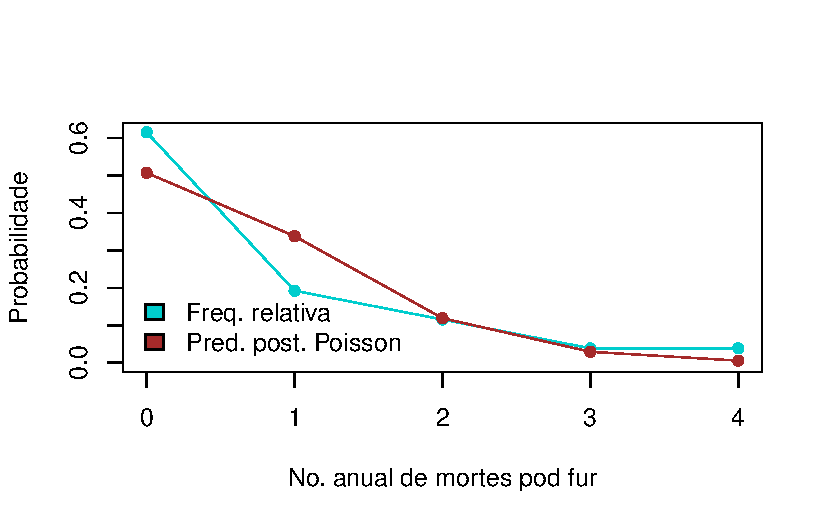
\includegraphics{misturas_files/figure-pdf/unnamed-chunk-2-1.pdf}

\begin{Shaded}
\begin{Highlighting}[]
\CommentTok{\# hiperparâmetros para rho}
\NormalTok{a }\OtherTok{=}\NormalTok{ b }\OtherTok{=} \DecValTok{1}

\CommentTok{\# hiperparâmetros para theta}
\NormalTok{r}\OtherTok{=}\NormalTok{.}\DecValTok{1}
\NormalTok{s}\OtherTok{=}\NormalTok{.}\DecValTok{1}

\CommentTok{\# tamanho da amostra}
\NormalTok{n }\OtherTok{\textless{}{-}} \FunctionTok{length}\NormalTok{(fur) }

\CommentTok{\# valores iniciais da cadeia}
\NormalTok{theta }\OtherTok{\textless{}{-}} \FunctionTok{mean}\NormalTok{(fur)}
\NormalTok{rho }\OtherTok{\textless{}{-}} \FunctionTok{mean}\NormalTok{(fur }\SpecialCharTok{==} \DecValTok{0}\NormalTok{)}

\CommentTok{\# amostrador de Gibbs}
\NormalTok{B }\OtherTok{\textless{}{-}} \DecValTok{50000}
\ControlFlowTok{for}\NormalTok{(i }\ControlFlowTok{in} \DecValTok{1}\SpecialCharTok{:}\NormalTok{B)\{}
  \CommentTok{\# simulando z}
\NormalTok{  z }\OtherTok{\textless{}{-}} \ConstantTok{NULL}
\NormalTok{  prob }\OtherTok{\textless{}{-}}\NormalTok{ rho[i]}\SpecialCharTok{/}\NormalTok{ ( (}\DecValTok{1}\SpecialCharTok{{-}}\NormalTok{rho[i])}\SpecialCharTok{*}\FunctionTok{dpois}\NormalTok{(}\DecValTok{0}\NormalTok{,theta[i]) }\SpecialCharTok{+}\NormalTok{ rho[i])}
  \ControlFlowTok{for}\NormalTok{(j }\ControlFlowTok{in} \DecValTok{1}\SpecialCharTok{:}\NormalTok{n)\{}
    \ControlFlowTok{if}\NormalTok{(fur[j] }\SpecialCharTok{\textgreater{}}\DecValTok{0}\NormalTok{)\{ z[j] }\OtherTok{\textless{}{-}} \DecValTok{0}\NormalTok{\} }\ControlFlowTok{else}\NormalTok{\{}
\NormalTok{      z[j] }\OtherTok{\textless{}{-}} \FunctionTok{rbinom}\NormalTok{(}\DecValTok{1}\NormalTok{,}\DecValTok{1}\NormalTok{,prob)}
\NormalTok{    \}}
\NormalTok{  \}}

  \CommentTok{\# simulando rho}
\NormalTok{  rho[i}\SpecialCharTok{+}\DecValTok{1}\NormalTok{] }\OtherTok{\textless{}{-}} \FunctionTok{rbeta}\NormalTok{( }\DecValTok{1}\NormalTok{, a }\SpecialCharTok{+} \FunctionTok{sum}\NormalTok{( z }\SpecialCharTok{*}\NormalTok{ (fur }\SpecialCharTok{==} \DecValTok{0}\NormalTok{)) , n}\SpecialCharTok{{-}} \FunctionTok{sum}\NormalTok{(z)}\SpecialCharTok{+}\NormalTok{ b )}
  
  \CommentTok{\# simulando theta}
\NormalTok{  theta[i}\SpecialCharTok{+}\DecValTok{1}\NormalTok{] }\OtherTok{\textless{}{-}} \FunctionTok{rgamma}\NormalTok{(}\DecValTok{1}\NormalTok{, }\FunctionTok{sum}\NormalTok{( fur}\SpecialCharTok{*}\NormalTok{(}\DecValTok{1}\SpecialCharTok{{-}}\NormalTok{z) ) }\SpecialCharTok{+}\NormalTok{ r,  n }\SpecialCharTok{{-}} \FunctionTok{sum}\NormalTok{(z) }\SpecialCharTok{+}\NormalTok{ s)}
\NormalTok{\}}
\end{Highlighting}
\end{Shaded}

Vamos descartar a metade das simulações e usar um \textbf{thinning}
igual a 15:

\begin{Shaded}
\begin{Highlighting}[]
\NormalTok{theta\_sim }\OtherTok{\textless{}{-}}\NormalTok{ theta[}\FunctionTok{seq}\NormalTok{(B}\SpecialCharTok{/}\DecValTok{2}\NormalTok{,B,}\DecValTok{15}\NormalTok{)]}
\NormalTok{rho\_sim }\OtherTok{\textless{}{-}}\NormalTok{ rho[}\FunctionTok{seq}\NormalTok{(B}\SpecialCharTok{/}\DecValTok{2}\NormalTok{,B,}\DecValTok{15}\NormalTok{)]}

\NormalTok{oo }\OtherTok{\textless{}{-}} \FunctionTok{par}\NormalTok{(}\AttributeTok{mfrow=}\FunctionTok{c}\NormalTok{(}\DecValTok{2}\NormalTok{,}\DecValTok{2}\NormalTok{))}
\FunctionTok{ts.plot}\NormalTok{(theta\_sim, }\AttributeTok{lwd =} \DecValTok{2}\NormalTok{)}
\FunctionTok{ts.plot}\NormalTok{(rho\_sim, }\AttributeTok{lwd =} \DecValTok{2}\NormalTok{)}
\FunctionTok{acf}\NormalTok{(theta\_sim)}
\FunctionTok{acf}\NormalTok{(rho\_sim)}
\end{Highlighting}
\end{Shaded}

\includegraphics{misturas_files/figure-pdf/unnamed-chunk-4-1.pdf}

Vamos estimar as probabilidade de ocorrerem \(k\) mortes via preditiva
posteriori:

\begin{Shaded}
\begin{Highlighting}[]
\CommentTok{\# tamanho do vetor simulado}
\NormalTok{Bs }\OtherTok{\textless{}{-}} \FunctionTok{length}\NormalTok{(theta\_sim)}

\NormalTok{x\_til }\OtherTok{\textless{}{-}} \FunctionTok{array}\NormalTok{( }\ConstantTok{NA\_real\_}\NormalTok{, }\FunctionTok{c}\NormalTok{(Bs,n))}
\ControlFlowTok{for}\NormalTok{(j }\ControlFlowTok{in} \DecValTok{1}\SpecialCharTok{:}\NormalTok{Bs)\{}
\NormalTok{  z }\OtherTok{\textless{}{-}} \FunctionTok{rbinom}\NormalTok{( n, }\DecValTok{1}\NormalTok{, rho\_sim[j])}
\NormalTok{  x\_til[j,] }\OtherTok{\textless{}{-}}\NormalTok{ (}\DecValTok{1}\SpecialCharTok{{-}}\NormalTok{z)}\SpecialCharTok{*}\FunctionTok{rpois}\NormalTok{(n, theta\_sim[j])}
\NormalTok{\}}

\CommentTok{\# probabilidades estimadas via ZIP}
\NormalTok{p\_zip }\OtherTok{\textless{}{-}} \FunctionTok{prop.table}\NormalTok{(}\FunctionTok{table}\NormalTok{(x\_til))}

\NormalTok{p\_zip}
\end{Highlighting}
\end{Shaded}

\begin{verbatim}
x_til
           0            1            2            3            4            5 
6.132850e-01 1.991371e-01 1.156615e-01 4.847492e-02 1.654285e-02 4.914402e-03 
           6            7            8 
1.476628e-03 4.153016e-04 9.228923e-05 
\end{verbatim}

Abaixo mostramos as probabilidades preditas do modelo ZIP, do modelo
Poisson a e frequência relativa.

\begin{Shaded}
\begin{Highlighting}[]
\NormalTok{r1 }\OtherTok{\textless{}{-}} \FunctionTok{sum}\NormalTok{(fur)}
\NormalTok{s1 }\OtherTok{\textless{}{-}} \FunctionTok{length}\NormalTok{(fur)}
\FunctionTok{plot}\NormalTok{(}\FunctionTok{table}\NormalTok{(fur)}\SpecialCharTok{/}\NormalTok{s1, }\AttributeTok{type=} \StringTok{\textquotesingle{}p\textquotesingle{}}\NormalTok{, }\AttributeTok{xlab=}\StringTok{\textquotesingle{}No. anual de mortes pod fur\textquotesingle{}}\NormalTok{, }\AttributeTok{ylab =} \StringTok{\textquotesingle{}Probabilidade\textquotesingle{}}\NormalTok{, }\AttributeTok{col =} \StringTok{\textquotesingle{}cyan3\textquotesingle{}}\NormalTok{, }\AttributeTok{pch=}\DecValTok{16}\NormalTok{)}
\FunctionTok{lines}\NormalTok{(}\DecValTok{0}\SpecialCharTok{:}\DecValTok{4}\NormalTok{,}\FunctionTok{table}\NormalTok{(fur)}\SpecialCharTok{/}\NormalTok{s1, }\AttributeTok{col =} \StringTok{\textquotesingle{}cyan3\textquotesingle{}}\NormalTok{)}
\FunctionTok{points}\NormalTok{(}\DecValTok{0}\SpecialCharTok{:}\DecValTok{4}\NormalTok{, }\FunctionTok{dnbinom}\NormalTok{(}\DecValTok{0}\SpecialCharTok{:}\DecValTok{4}\NormalTok{, }\AttributeTok{size =}\NormalTok{ r1, }\AttributeTok{prob =}\NormalTok{ s1}\SpecialCharTok{/}\NormalTok{(}\DecValTok{1}\SpecialCharTok{+}\NormalTok{s1)), }\AttributeTok{pch=}\DecValTok{16}\NormalTok{, }\AttributeTok{col =} \StringTok{\textquotesingle{}brown\textquotesingle{}}\NormalTok{)}
\FunctionTok{lines}\NormalTok{(}\DecValTok{0}\SpecialCharTok{:}\DecValTok{4}\NormalTok{, }\FunctionTok{dnbinom}\NormalTok{(}\DecValTok{0}\SpecialCharTok{:}\DecValTok{4}\NormalTok{, }\AttributeTok{size =}\NormalTok{ r1, }\AttributeTok{prob =}\NormalTok{ s1}\SpecialCharTok{/}\NormalTok{(}\DecValTok{1}\SpecialCharTok{+}\NormalTok{s1)), }\AttributeTok{col =} \StringTok{\textquotesingle{}brown\textquotesingle{}}\NormalTok{)}
\FunctionTok{points}\NormalTok{(}\FunctionTok{names}\NormalTok{(p\_zip),p\_zip, }\AttributeTok{pch=}\DecValTok{16}\NormalTok{,}\AttributeTok{col =} \StringTok{\textquotesingle{}magenta\textquotesingle{}}\NormalTok{)}
\FunctionTok{lines}\NormalTok{(}\FunctionTok{names}\NormalTok{(p\_zip),p\_zip,}\AttributeTok{col =} \StringTok{\textquotesingle{}magenta\textquotesingle{}}\NormalTok{)}

\FunctionTok{legend}\NormalTok{(}\StringTok{\textquotesingle{}bottomleft\textquotesingle{}}\NormalTok{,}\FunctionTok{c}\NormalTok{(}\StringTok{\textquotesingle{}Freq. relativa\textquotesingle{}}\NormalTok{,}\StringTok{\textquotesingle{}Pred. post. Poisson\textquotesingle{}}\NormalTok{, }\StringTok{\textquotesingle{}Pred. post. ZIP\textquotesingle{}}\NormalTok{), }\AttributeTok{fill=}\FunctionTok{c}\NormalTok{(}\StringTok{\textquotesingle{}cyan3\textquotesingle{}}\NormalTok{,}\StringTok{\textquotesingle{}brown\textquotesingle{}}\NormalTok{, }\StringTok{\textquotesingle{}magenta\textquotesingle{}}\NormalTok{), }\AttributeTok{bty=}\StringTok{\textquotesingle{}n\textquotesingle{}}\NormalTok{)}
\end{Highlighting}
\end{Shaded}

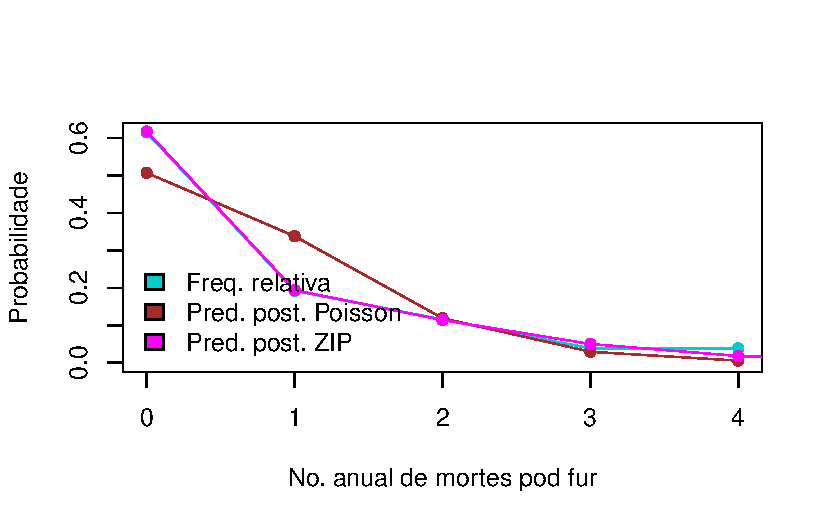
\includegraphics{misturas_files/figure-pdf/unnamed-chunk-6-1.pdf}

\subsection{Exercício}\label{exercuxedcio-1}

Abaixo, segue o número anual de tornados em Lafayette Parish, Louisiana,
entre 1950 e 2012.

\begin{Shaded}
\begin{Highlighting}[]
\NormalTok{tor }\OtherTok{\textless{}{-}} \FunctionTok{c}\NormalTok{(}\DecValTok{0}\NormalTok{, }\DecValTok{0}\NormalTok{,}\DecValTok{0}\NormalTok{, }\DecValTok{1}\NormalTok{, }\DecValTok{0}\NormalTok{, }\DecValTok{0}\NormalTok{, }\DecValTok{0}\NormalTok{, }\DecValTok{1}\NormalTok{, }\DecValTok{0}\NormalTok{, }\DecValTok{0}\NormalTok{,}
\DecValTok{1}\NormalTok{, }\DecValTok{0}\NormalTok{, }\DecValTok{0}\NormalTok{, }\DecValTok{0}\NormalTok{, }\DecValTok{1}\NormalTok{, }\DecValTok{1}\NormalTok{, }\DecValTok{0}\NormalTok{, }\DecValTok{0}\NormalTok{, }\DecValTok{0}\NormalTok{, }\DecValTok{2}\NormalTok{,}
\DecValTok{0}\NormalTok{, }\DecValTok{0}\NormalTok{, }\DecValTok{0}\NormalTok{, }\DecValTok{0}\NormalTok{, }\DecValTok{1}\NormalTok{, }\DecValTok{3}\NormalTok{, }\DecValTok{0}\NormalTok{, }\DecValTok{2}\NormalTok{, }\DecValTok{1}\NormalTok{, }\DecValTok{0}\NormalTok{,}
\DecValTok{1}\NormalTok{, }\DecValTok{0}\NormalTok{, }\DecValTok{0}\NormalTok{, }\DecValTok{1}\NormalTok{, }\DecValTok{0}\NormalTok{, }\DecValTok{1}\NormalTok{, }\DecValTok{0}\NormalTok{, }\DecValTok{0}\NormalTok{, }\DecValTok{2}\NormalTok{, }\DecValTok{1}\NormalTok{,}
\DecValTok{0}\NormalTok{, }\DecValTok{1}\NormalTok{, }\DecValTok{2}\NormalTok{, }\DecValTok{0}\NormalTok{, }\DecValTok{0}\NormalTok{, }\DecValTok{1}\NormalTok{, }\DecValTok{0}\NormalTok{, }\DecValTok{1}\NormalTok{, }\DecValTok{2}\NormalTok{, }\DecValTok{0}\NormalTok{,}
\DecValTok{0}\NormalTok{, }\DecValTok{0}\NormalTok{, }\DecValTok{3}\NormalTok{, }\DecValTok{0}\NormalTok{, }\DecValTok{2}\NormalTok{, }\DecValTok{0}\NormalTok{, }\DecValTok{1}\NormalTok{, }\DecValTok{1}\NormalTok{, }\DecValTok{3}\NormalTok{, }\DecValTok{0}\NormalTok{,}
\DecValTok{1}\NormalTok{, }\DecValTok{1}\NormalTok{, }\DecValTok{1}\NormalTok{)}
\end{Highlighting}
\end{Shaded}

\begin{itemize}
\item
  Ajuste o modelo Poisson.
\item
  Ajuste o modelo Poisson inflado de zeros.
\end{itemize}

\section{Mistura escalonada de
normais}\label{mistura-escalonada-de-normais}

\section{Misturas finitas com
número}\label{misturas-finitas-com-nuxfamero}

Dizemos que \(X|\boldsymbol{\theta},\boldsymbol{p},\kappa\) é um modelo
de mistura finito se sua função de densidade/probabilidade é dada por

\[f(x| \boldsymbol{\theta},\boldsymbol{p} ,\kappa )=\sum_{k=1}^\kappa p_k f_k(x|\boldsymbol{\theta}_k).\]

Cada função \(f(.|\boldsymbol{\theta}_k)\) é denominada componente da
mistura e o número de componentes pode ser desconhecido.

Assim como o modelo com zeros inflacionados, podemos utilizar uma
variável latente
\(\textbf{z}_i|\kappa=(z_{i,1},\ldots,z_{i,\kappa})\sim\hbox{Multinomial}(p_1\ldots,p_\kappa|\sum_{k=1}^\kappa z_{ik}=1)\),
obtendo o seguinte modelo aumentado

\[f(x_i|\boldsymbol{\theta},\textbf{z}_i,\kappa)=\prod_{k=1}^\kappa \left[f\left(x_i|\boldsymbol{\theta}_k\right)\right]^{z_{i,k}}\]

A função de verossimilhança aumentada para este modelo é

\[\prod_{i=1}^n f(x_i|\boldsymbol{\theta},\textbf{z}_i,\kappa)=\prod_{i=1}^n\prod_{k=1}^\kappa \left[f\left(x_i|\boldsymbol{\theta}_k\right)\right]^{z_{i,k}}.\]

Considere as prioris
\(\pi(\boldsymbol{\theta}|\kappa)=\prod_{k=1}^\kappa \pi(\boldsymbol{\theta}_k)\)
e \(\textbf{p}|\kappa\sim\hbox{Dirichlet}(a_1,\ldots,a_\kappa)\), onde
\[f(\textbf{p}|\kappa)\propto \prod_{k=1}^\kappa p_k^{a_k-1}\] com
\(\sum_{k=1}^\kappa p_k=1\). As condicionais completas para este
problema são

\begin{itemize}
\item
  \(\begin{align}f(\boldsymbol{\theta}_k|resto)\propto \prod_{i:z_{i,k}=1}f(x_i|\boldsymbol{\theta}_k)\pi(\boldsymbol{\theta}_k)\end{align}\)
\item
  \(\begin{align}f(\textbf{z}_i|resto)\propto \prod_{k=1}^\kappa \left[p_kf(x_i|\boldsymbol{\theta}_k)\right]^{z_{i,k}}\end{align}\)
  ou seja,
  \(\textbf{z}_i|rest\sim\hbox{Multinomial}(\tilde{p}_1,\ldots,\tilde{p}_\kappa)\),
  onde
\end{itemize}

\[\tilde{p}_k=\frac{p_kf(x_i|\boldsymbol{\theta}_k)}{\sum_{k=1}^\kappa p_kf(x_i|\boldsymbol{\theta}_k)}\]
*
\(f(\textbf{p}|resto)\propto \prod_{k=1}^\kappa p_k^{\sum_{i=1}^n z_{i,k}+a_k-1}\),
ou seja
\(\textbf{p}|resto\sim\hbox{Dirichlet}(a_1+\sum_{i=1}^n z_{i,1},\ldots,a_\kappa+\sum_{i=1}^n z_{i,\kappa})\)

Se necessário, podemos atrbuir a priori
\[\pi(\kappa)=\frac{1}{M},\kappa=1,2,\ldots,M\] para obter a condicional
completa
\[\pi(\kappa|resto)=\frac{\prod_{i=1}^n\prod_{k=1}^\kappa f(x_i|\boldsymbol{\theta}_k)^{z_{i,k}}\pi(\boldsymbol{\theta}_k)\pi(\textbf{p}|\kappa)\pi(\textbf{z}_i|\kappa)}{\sum_{\kappa=1}^M \prod_{i=1}^n\prod_{k=1}^\kappa f(x_i|\boldsymbol{\theta}_k)^{z_{i,k}}\pi(\boldsymbol{\theta}_k)\pi(\textbf{p}|\kappa)\pi(\textbf{z}_i|\kappa)},\kappa=1,\ldots,M.\]

\subsection{O velho fiel}\label{o-velho-fiel}

O banco de dados \texttt{faithful} mostra a duração e o tempo até a
próxima erupção do geiser Velho Fiel, no parque Yellowstone. Abaixo
mostramos o diagrama do tempo de espera entre erupções

\begin{Shaded}
\begin{Highlighting}[]
\FunctionTok{hist}\NormalTok{(faithful}\SpecialCharTok{$}\NormalTok{waiting)}
\end{Highlighting}
\end{Shaded}

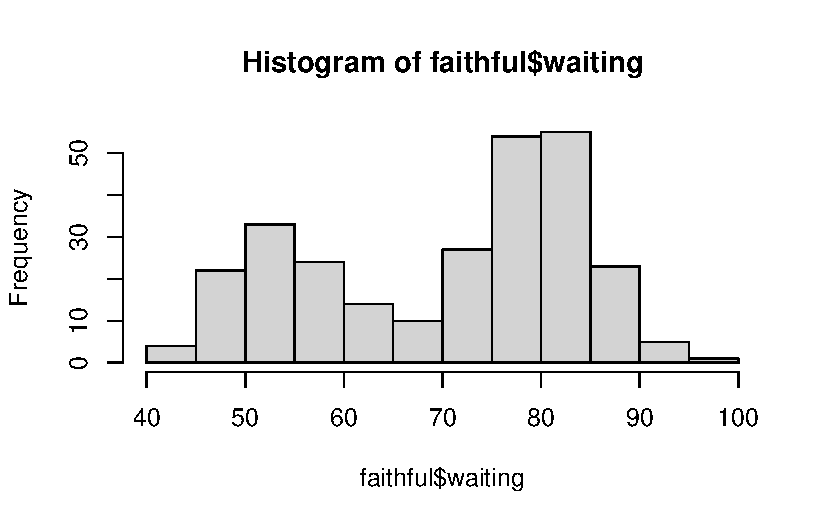
\includegraphics{misturas_files/figure-pdf/unnamed-chunk-8-1.pdf}

É possível notar classes, uma com tempo e entre erupções menor que 70
com tempo maior. Temos as seguintes estimativas iniciais:

\begin{Shaded}
\begin{Highlighting}[]
\DocumentationTok{\#\# elementos na classe 1}
\NormalTok{x }\OtherTok{\textless{}{-}}\NormalTok{ faithful}\SpecialCharTok{$}\NormalTok{waiting}
\NormalTok{z }\OtherTok{\textless{}{-}}\NormalTok{ x }\SpecialCharTok{\textless{}} \DecValTok{70}
\CommentTok{\# proporção na classe 1}
\FunctionTok{mean}\NormalTok{(z)}
\end{Highlighting}
\end{Shaded}

\begin{verbatim}
[1] 0.3786765
\end{verbatim}

\begin{Shaded}
\begin{Highlighting}[]
\CommentTok{\# média e desvio padrão na classe 1}
\FunctionTok{mean}\NormalTok{( x[z])}
\end{Highlighting}
\end{Shaded}

\begin{verbatim}
[1] 55.15534
\end{verbatim}

\begin{Shaded}
\begin{Highlighting}[]
\FunctionTok{sd}\NormalTok{( x[z])}
\end{Highlighting}
\end{Shaded}

\begin{verbatim}
[1] 6.266558
\end{verbatim}

\begin{Shaded}
\begin{Highlighting}[]
\DocumentationTok{\#\# elementos na classe 2}
\CommentTok{\# proporção na classe 2}
\FunctionTok{mean}\NormalTok{(z}\SpecialCharTok{==}\NormalTok{F)}
\end{Highlighting}
\end{Shaded}

\begin{verbatim}
[1] 0.6213235
\end{verbatim}

\begin{Shaded}
\begin{Highlighting}[]
\CommentTok{\# média e desvio padrão na classe 2}
\FunctionTok{mean}\NormalTok{( x[z}\SpecialCharTok{==}\NormalTok{F])}
\end{Highlighting}
\end{Shaded}

\begin{verbatim}
[1] 80.49112
\end{verbatim}

\begin{Shaded}
\begin{Highlighting}[]
\FunctionTok{sd}\NormalTok{( x[z}\SpecialCharTok{==}\NormalTok{F])}
\end{Highlighting}
\end{Shaded}

\begin{verbatim}
[1] 5.456667
\end{verbatim}

Vamos considerar que as duas componentes possuem distribuição normal.
Para cada componente, teremos as seguintes prioris:

\[\pi(\mu_i,\phi_i)=\frac{\phi^{1/2}_i}{\sqrt{2\pi C}}e^{-\frac{\phi_i}{2C}(\mu_i-m_i)^2}\frac{b^a}{\Gamma(a)}\phi_i^{a-1}e^{b\phi_i},\]

\[p\sim\hbox{Beta}(r,s)\]

\[z_i\sim\hbox{Bernoulli}(p)\]

O modelo aumentado é
\[f(x_i|\mu,\phi,z_{i})=\left[\frac{\phi_1^{1/2}}{\sqrt{2\pi}}e^{-\frac{\phi_1}{2}(x_i-\mu_1)}\right]^{z_i}\left[\frac{\phi_2^{1/2}}{\sqrt{2\pi}}e^{-\frac{\phi_2}{2}(x_i-\mu_2)}\right]^{1-z_i}\]
As condicionais completas são:

\[\begin{align}f(\mu_1|resto) &\propto \exp\left\{-\frac{\phi_1}{2}\sum_{i=1}^n z_i(x_i-\mu_1)^2\right\}\exp\left\{-\frac{\phi_1}{2C} z_i(\mu_1-m_1)^2\right\}\\&\propto \exp\left\{-\frac{\phi_1}{2}\left(\sum_{i=1}^n z_i+C^{-1}\right) \left(\mu_1-\frac{\sum_{i=1}^{n}x_iz_i+m_1C^{-1}}{\sum_{i=1}^n z_i+C^{-1}}\right)^2\right\}\end{align}\]

\[\begin{align}f(\mu_2|resto) &\propto \exp\left\{-\frac{\phi_2}{2}\sum_{i=1}^n (1-z_i)(x_i-\mu_2)^2\right\}\exp\left\{-\frac{\phi_2}{2C} (1-z_i)(\mu_2-m_2)^2\right\}\\&\propto \exp\left\{-\frac{\phi_2}{2}\left(\sum_{i=1}^n (1-z_i)+C^{-1}\right) \left(\mu_2-\frac{\sum_{i=1}^{n}x_i(1-z_i)+m_1C^{-1}}{\sum_{i=1}^n (1-z_i)+C^{-1}}\right)^2\right\}\end{align}\]

\[\begin{align}f(\phi_2|resto)&\propto \phi_2^{-\frac{1}{2}\sum_{i=1}^{n}z_i}
e^{-\frac{\phi_2}{2}\sum_{i=1}^n (1-z_i)(x_i-\mu_2)^2}\phi^{-1/2}_2e^{-\frac{\phi_2}{2}(\mu_2-m_2)^2}\phi_2^{a/2-1}e^{-\phi_2 b/2}\\ &\propto \phi_2^{\frac{1}{2}(1+a+\sum_{i=1}^{n}(1-z_i)-1}e^{-\frac{\phi_2}{2}[\sum_{i=1}^n(1-z_i)(x_i-\mu_2)^2 +(\mu_2-m_2)^2 + b]}\end{align}\]
\[\begin{align}f(\phi_1|resto)&\propto \phi^{-\frac{1}{2}\sum_{i=1}^{n}z_i}
e^{-\frac{\phi_1}{2}\sum_{i=1}^n z_i(x_i-\mu_1)^2}\phi^{-1/2}e^{-\frac{\phi_1}{2}(\mu_1-m_1)^2}\phi_1^{a/2-1}e^{-\phi_1 b/2}\\ &\propto \phi_1^{\frac{1}{2}(1+a+\sum_{i=1}^{n}z_i)-1}e^{-\frac{\phi_1}{2}[\sum_{i=1}^nz_i(x_i-\mu_1)^2 +(\mu_1-m_1)^2 + b]}\end{align}\]

\[\begin{align}f(p|resto)\propto \prod_{i=1}^n p^{z_i}(1-p)^{1-z_i}p^{r-1}(1-p)^{s-1}\propto p^{r+\sum_{i=1}^n z_i-1}(1-p)^{s+\sum_{i=1}^n (1-z_i)-1}\end{align}\]

\[f(z_i|resto)\propto\left[ p\frac{\phi_1^{1/2}}{\sqrt{2\pi}}e^{-\frac{\phi_1}{2}(x_i-\mu_1)^2}\right]^{z_i}\left[ (1-p)\frac{\phi_2^{1/2}}{\sqrt{2\pi}}e^{-\frac{\phi_2}{2}(x_i-\mu_2)^2}\right]^{1-z_i}\]

Abaixo implementamos o amostrador de Gibbs

\begin{Shaded}
\begin{Highlighting}[]
\NormalTok{B }\OtherTok{\textless{}{-}} \DecValTok{50000}

\CommentTok{\# hiperparmametros}
\NormalTok{m1 }\OtherTok{\textless{}{-}} \DecValTok{65}
\NormalTok{m2 }\OtherTok{\textless{}{-}} \DecValTok{80}
\NormalTok{C }\OtherTok{\textless{}{-}} \DecValTok{1000}
\NormalTok{r}\OtherTok{=} \DecValTok{4}\NormalTok{; s }\OtherTok{=} \DecValTok{6}
\NormalTok{a }\OtherTok{=} \DecValTok{1}\NormalTok{; b }\OtherTok{=}\NormalTok{ .}\DecValTok{1}

\CommentTok{\# valores iniciais}
\NormalTok{z }\OtherTok{\textless{}{-}}\NormalTok{ x }\SpecialCharTok{\textless{}} \DecValTok{70}
\NormalTok{phi1 }\OtherTok{\textless{}{-}} \DecValTok{1}\SpecialCharTok{/}\DecValTok{36}
\NormalTok{phi2 }\OtherTok{\textless{}{-}} \DecValTok{1}\SpecialCharTok{/}\DecValTok{25}
\NormalTok{mu1 }\OtherTok{=}\NormalTok{ mu2 }\OtherTok{=}\NormalTok{  p }\OtherTok{=} \ConstantTok{NULL}

\ControlFlowTok{for}\NormalTok{(i }\ControlFlowTok{in} \DecValTok{1}\SpecialCharTok{:}\NormalTok{B)\{}
  \CommentTok{\# mu dado o resto}
\NormalTok{  m1\_post }\OtherTok{\textless{}{-}}\NormalTok{ ( }\FunctionTok{sum}\NormalTok{(x}\SpecialCharTok{*}\NormalTok{z) }\SpecialCharTok{+}\NormalTok{ m1}\SpecialCharTok{/}\NormalTok{C) }\SpecialCharTok{/}\NormalTok{ ( }\FunctionTok{sum}\NormalTok{(z) }\SpecialCharTok{+} \DecValTok{1}\SpecialCharTok{/}\NormalTok{C )}
\NormalTok{  m2\_post }\OtherTok{\textless{}{-}}\NormalTok{ ( }\FunctionTok{sum}\NormalTok{(x}\SpecialCharTok{*}\NormalTok{(}\DecValTok{1}\SpecialCharTok{{-}}\NormalTok{z)) }\SpecialCharTok{+}\NormalTok{ m1}\SpecialCharTok{/}\NormalTok{C) }\SpecialCharTok{/}\NormalTok{ ( }\FunctionTok{sum}\NormalTok{(}\DecValTok{1}\SpecialCharTok{{-}}\NormalTok{z) }\SpecialCharTok{+} \DecValTok{1}\SpecialCharTok{/}\NormalTok{C )}
\NormalTok{  s1\_post }\OtherTok{\textless{}{-}} \DecValTok{1} \SpecialCharTok{/}\NormalTok{ ( ( }\FunctionTok{sum}\NormalTok{(z) }\SpecialCharTok{+} \DecValTok{1}\SpecialCharTok{/}\NormalTok{C )}\SpecialCharTok{*}\NormalTok{phi1[i] )}
\NormalTok{  s2\_post }\OtherTok{\textless{}{-}} \DecValTok{1} \SpecialCharTok{/}\NormalTok{ ( ( }\FunctionTok{sum}\NormalTok{(}\DecValTok{1}\SpecialCharTok{{-}}\NormalTok{z) }\SpecialCharTok{+} \DecValTok{1}\SpecialCharTok{/}\NormalTok{C )}\SpecialCharTok{*}\NormalTok{phi2[i] )}
  
\NormalTok{  mu1[i}\SpecialCharTok{+}\DecValTok{1}\NormalTok{] }\OtherTok{\textless{}{-}} \FunctionTok{rnorm}\NormalTok{(}\DecValTok{1}\NormalTok{, m1\_post, }\FunctionTok{sqrt}\NormalTok{( s1\_post) )}
\NormalTok{  mu2[i}\SpecialCharTok{+}\DecValTok{1}\NormalTok{] }\OtherTok{\textless{}{-}} \FunctionTok{rnorm}\NormalTok{(}\DecValTok{1}\NormalTok{, m2\_post, }\FunctionTok{sqrt}\NormalTok{( s2\_post) )}
  
  \CommentTok{\# phi dado resto}
\NormalTok{  phi1[i}\SpecialCharTok{+}\DecValTok{1}\NormalTok{] }\OtherTok{\textless{}{-}} \FunctionTok{rgamma}\NormalTok{(}\DecValTok{1}\NormalTok{, }\DecValTok{1} \SpecialCharTok{+}\NormalTok{ a }\SpecialCharTok{+} \FunctionTok{sum}\NormalTok{(z), }\FunctionTok{sum}\NormalTok{( z}\SpecialCharTok{*}\NormalTok{(x }\SpecialCharTok{{-}}\NormalTok{ mu1[i}\SpecialCharTok{+}\DecValTok{1}\NormalTok{])}\SpecialCharTok{\^{}}\DecValTok{2}\NormalTok{ ) }\SpecialCharTok{+}\NormalTok{ (mu1[i}\SpecialCharTok{+}\DecValTok{1}\NormalTok{]}\SpecialCharTok{{-}}\NormalTok{m1)}\SpecialCharTok{\^{}}\DecValTok{2} \SpecialCharTok{+}\NormalTok{ b)}
\NormalTok{  phi2[i}\SpecialCharTok{+}\DecValTok{1}\NormalTok{] }\OtherTok{\textless{}{-}} \FunctionTok{rgamma}\NormalTok{(}\DecValTok{1}\NormalTok{, }\DecValTok{1} \SpecialCharTok{+}\NormalTok{ a }\SpecialCharTok{+} \FunctionTok{sum}\NormalTok{(}\DecValTok{1}\SpecialCharTok{{-}}\NormalTok{z), }\FunctionTok{sum}\NormalTok{( (}\DecValTok{1}\SpecialCharTok{{-}}\NormalTok{z)}\SpecialCharTok{*}\NormalTok{(x }\SpecialCharTok{{-}}\NormalTok{ mu2[i}\SpecialCharTok{+}\DecValTok{1}\NormalTok{])}\SpecialCharTok{\^{}}\DecValTok{2}\NormalTok{ ) }\SpecialCharTok{+}\NormalTok{ (mu2[i}\SpecialCharTok{+}\DecValTok{1}\NormalTok{]}\SpecialCharTok{{-}}\NormalTok{m2)}\SpecialCharTok{\^{}}\DecValTok{2} \SpecialCharTok{+}\NormalTok{ b)}
  
  \CommentTok{\# p dado resto}
\NormalTok{  p[i}\SpecialCharTok{+}\DecValTok{1}\NormalTok{] }\OtherTok{\textless{}{-}} \FunctionTok{rbeta}\NormalTok{(}\DecValTok{1}\NormalTok{, r }\SpecialCharTok{+} \FunctionTok{sum}\NormalTok{(z), s }\SpecialCharTok{+} \FunctionTok{sum}\NormalTok{(}\DecValTok{1}\SpecialCharTok{{-}}\NormalTok{z) )}
  
  \CommentTok{\# z dado resto}
\NormalTok{  aux1 }\OtherTok{\textless{}{-}}\NormalTok{ p[i}\SpecialCharTok{+}\DecValTok{1}\NormalTok{]}\SpecialCharTok{*}\FunctionTok{dnorm}\NormalTok{(x,mu1[i}\SpecialCharTok{+}\DecValTok{1}\NormalTok{], }\DecValTok{1}\SpecialCharTok{/}\FunctionTok{sqrt}\NormalTok{(phi1[i}\SpecialCharTok{+}\DecValTok{1}\NormalTok{]))}
\NormalTok{  aux2 }\OtherTok{\textless{}{-}}\NormalTok{ (}\DecValTok{1}\SpecialCharTok{{-}}\NormalTok{p[i}\SpecialCharTok{+}\DecValTok{1}\NormalTok{])}\SpecialCharTok{*}\FunctionTok{dnorm}\NormalTok{(x,mu2[i}\SpecialCharTok{+}\DecValTok{1}\NormalTok{], }\DecValTok{1}\SpecialCharTok{/}\FunctionTok{sqrt}\NormalTok{(phi2[i}\SpecialCharTok{+}\DecValTok{1}\NormalTok{]))}
  
\NormalTok{  z }\OtherTok{\textless{}{-}} \FunctionTok{rbinom}\NormalTok{(}\FunctionTok{length}\NormalTok{(x), }\DecValTok{1}\NormalTok{, aux1}\SpecialCharTok{/}\NormalTok{( aux1 }\SpecialCharTok{+}\NormalTok{ aux2))}
\NormalTok{\}}
\CommentTok{\# }
\end{Highlighting}
\end{Shaded}

\begin{Shaded}
\begin{Highlighting}[]
\FunctionTok{hist}\NormalTok{(mu1[}\FunctionTok{seq}\NormalTok{(B}\SpecialCharTok{/}\DecValTok{2}\NormalTok{,B,}\DecValTok{30}\NormalTok{)])}
\end{Highlighting}
\end{Shaded}

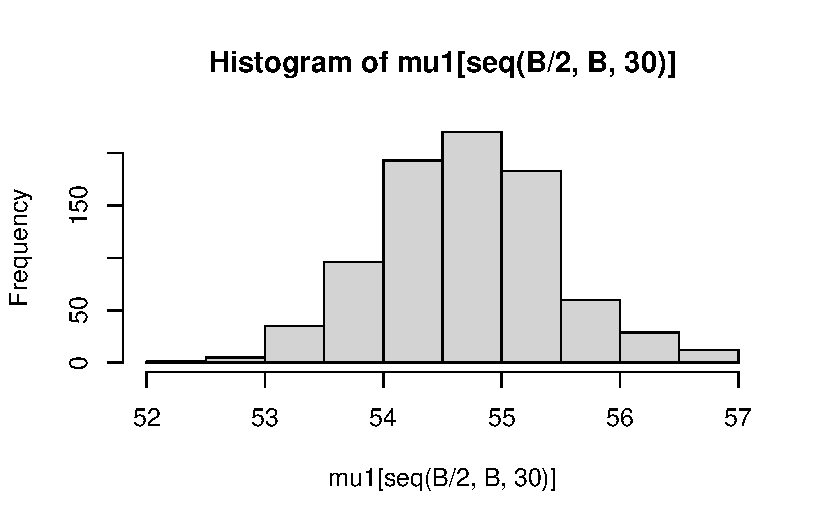
\includegraphics{misturas_files/figure-pdf/unnamed-chunk-12-1.pdf}

\begin{Shaded}
\begin{Highlighting}[]
\FunctionTok{hist}\NormalTok{(mu2[}\FunctionTok{seq}\NormalTok{(B}\SpecialCharTok{/}\DecValTok{2}\NormalTok{,B,}\DecValTok{30}\NormalTok{)])}
\end{Highlighting}
\end{Shaded}

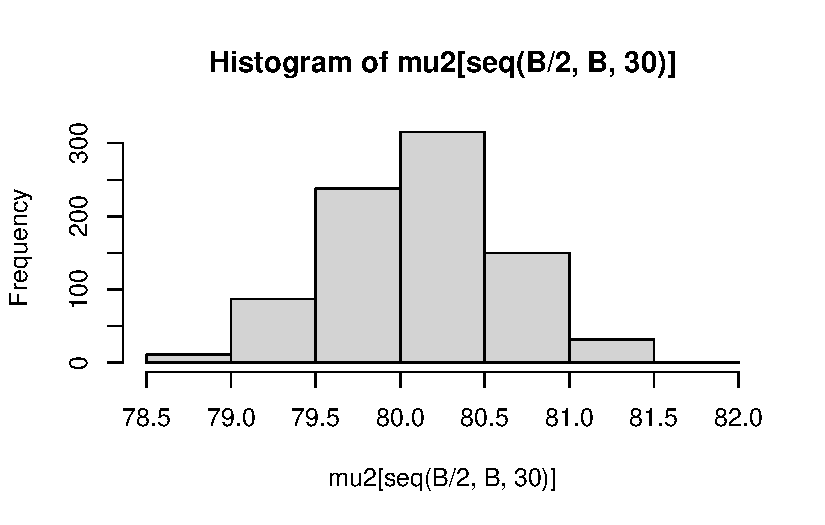
\includegraphics{misturas_files/figure-pdf/unnamed-chunk-12-2.pdf}

\bookmarksetup{startatroot}

\chapter{O modelo Poisson}\label{o-modelo-poisson-1}

\section{Sobre o modelo}\label{sobre-o-modelo-1}

Seja \(N(t)\) o número de ocorrências observadas no intervalo de tempo
\([0,t]\) (considere que \(N(0)=0\)). Note que o número de eventos no
intervalo \((s,t]\) é dado por \(N(t)-N(s)\).

Dizemos que \(N(t)\) tem incrementos independentes se, para quaisquer
intervalos disjuntos \((s_0,t_0]\) e \((s_1,t_1]\), as contagens
\(N(t_0)-N(s_0)\) e \(N(t_1)-N(s_1)\) são independentes.

\(N(t)\) é denominado Processo de Poisson quando ele possui incrementos
indepentes e, para qualquer intervalo \((s,t]\),

\[P(N(t)-N(s)=x)=\frac{e^{-\lambda(t-s)[\lambda(t-s)]^x}}{x!},\] onde
\(x=0,1,\ldots\) e \(\lambda>0\). Isto implica que
\[E(N(t))=\lambda t,\] ou seja, o número esperado de ocorrências até o
tempo \(t\) é diretamente proporcional à \(t\) e \(\lambda\) representa
a taxa de crescimento. Para este processo, é verdade que
\[\lim_{\delta\rightarrow 0}P(N(t+\delta)-N(t)>1)=0,\] ou seja, não é
possível observar duas ou mais ocorrências simultaneamente.

Em geral, os experimentos são desenhados para registrar contagens em
intervalos regulares e disjuntos de tempo, como semanas ou anos.
Considere que tais intervalos são
\([0,s_1],(s_1,s_2],\ldots,(s_{n-1},t]\) e seja \(c\) o comprimento
destes intervalos. Em geral, os dados são apresentados como contagens
dentro destes intevalos, gerando as seguintes variáveis:

\begin{itemize}
\tightlist
\item
  \(X_1=N(s_1)\sim\hbox{Poisson}(\lambda c)\)
\item
  \(X_2=N(s_2)-N(s_1)\sim\hbox{Poisson}(\lambda c)\)
\item
  \(\cdots\)
\item
  \(X_n=N(t)-N(s_{n-1})\sim\hbox{Poisson}(\lambda c)\) ou seja,
  \(X_1,\ldots,X_n\) são uma amostra aleatória do modelo
  Poisson(\(\lambda c\)). Na prática, \(c=1\) por ser a unidade de
  medida de tempo associada ao experimento (uma semana, um ano, etc).
\end{itemize}

\subsection{Tempos de chegadas e tempos de
espera}\label{tempos-de-chegadas-e-tempos-de-espera-1}

Para um processo de Poisson \(N(t)\), definimos o tempo de chegadas como
o tempo entre duas observações consecutivas. Denotaremos o tempo de
chegadas entre a \(i\)-ésima e a \(i-1\) ésima ocorrência por \(T_i\).

É possível mostrar que \(T_i\) é independente de \(T_j\), para
\(i\neq j\) e que \(T_i\sim\hbox{Exponencial}(\lambda)\). Por isso, para
uma amostra aleatória de um modelo Exponencial(\(\lambda\)), o parâmetro
\(\lambda\) é demoninado taxa.

Definimos por tempo de espera da ocorrência \(n\) como o tempo
transcorrido desde o início do processo até a ocorrência do \(n\)-ésimo
evento. Este tempo de espera é denotado por \(S_n\). Exsitem dois
resultados importantes relacionados ao tempo de espera:

\begin{itemize}
\item
  \(S_n=T_1+\cdots+T_n\) tem distribuição Gama(\(n,\lambda\))
\item
  Dado que \(N(t)=n\), os tempos de espera dos eventos estão
  uniformemente distribuídos dentro do intervalo \((0,t)\).
\end{itemize}

\subsection{Ocorrências de diversas
classes}\label{ocorruxeancias-de-diversas-classes-1}

Suponha que as ocorrências observadas podem ser classificadas em \(k\)
categorias. Suponha que qualquer ocorrência tem probabilidade \(p_j\) de
pertencer a categoria \(j\). Então

\begin{itemize}
\item
  O número de ocorrências da classe \(j\) é um processo de Poisson com
  taxa \(\lambda p_j\)
\item
  O número de ocorrências da classe \(j\) é independente do número de
  ocorrências da classe \(i\), com \(i\neq j\)
\end{itemize}

\subsection{O processo de Poisson
Espacial}\label{o-processo-de-poisson-espacial-1}

Seja \(N(A)\) o número de ocorrências observadas em uma região de área
\(A\). \(N(A)\) é denominado Processo de Poisson Espacial quando
\(N(A)\sim\hbox{Poisson}(\lambda A)\) e, para duas regiões distintas de
áreas \(B\) e \(C\), \(N(B)\) e \(N(C)\) são independentes.

Note que, para um Processo de Poisson Espaical, dado \(N(A)=n\) as \(n\)
ocorrências estão uniformemente distribuídas dentro da região \(A\)

\section{Verossimilhança e priori
conjugada}\label{verossimilhanuxe7a-e-priori-conjugada-1}

Seja \(X_1,\ldots,X_n\) uma amostra aleatória do modelo
Poisson\((\lambda)\). A verossimilhança deste modelo é dada por

\[L(\theta)=\frac{e^{-n\theta}\theta^{\sum_{i=1}^{n}x_i}}{\prod_{i=1}^{n}x_i!}\propto \theta^{\sum_{i=1}^n x_i}e^{-n\theta}.\]
O modelo Poisson pertence à família exponencial e sua priori conjugada é
\(\theta\sim\hbox{Gama}(r,s)\) e a posteriori é
\(\hbox{Gama}(r+\sum_{i=1}^n x_i+r, s+n)\), conforme já discutido na
Introdução. Os hiperparâmetros \(r\) e \(s\) podem ser interpretados
como o total da contagem e o tamanho da amostra a priori.

A média da posteriori é
\[E(\theta|\mathbf{x})=\frac{\sum_{i=1}^{n}x_i+r}{n+s}=\frac{n}{n+s}\bar{x}+\frac{s}{n+s}E(\theta),\]
onde fica claro que este estimador é uma média ponderada das informações
provenientes das duas fontes de informação (sendo \(\bar{x}\) a
estimativa de máxima verossimilhança e \(E(\theta)\) a média a priori).

Se \(n\gg s\), então a média a posteriori dará maior peso para a
informação dos dados.

\section{Preditiva a posteriori}\label{preditiva-a-posteriori-1}

A inferência bayesiana é baseada em duas fontes de informação:
verossimilhança e priori. Já discutimos que, na maioria dos casos,
estamos interessados em deixar a verossimilhança ter mais peso na
posteriori. Agora, vamos discutir como verificar se a verossimilhança é
adequada ao problema.

Seja \(\boldsymbol{x}=\{x_1,\ldots,x_n\}\) a amostra observada e
\(f(\theta|\boldsymbol{x})\) a posteriori obtida. Supondo que a
informação sobre os parâmetros foi capturada de forma adequada, é de se
esperar que uma nova observação \(x^*\) se comporte de modo semelhante a
amostra observada. Podemos então obter a seguinte distribuição,
denominada preditiva a posteriori:

\[\begin{align}f(x^*|\boldsymbol{x})=\int f(x^*|\theta)f(\theta|\boldsymbol{x})d\theta.\end{align}\]

Podemos comparar as características preditiva a posteriori com
estatísticas livres de modelos como box-plots, histogramas, etc.

\textbf{Preditiva a posteriori para o modelo Poisson}

Para o modelo Poisson(\(\lambda\)) e para a posteriori
Gama\((r_1,s_1)\), onde \(r_1=r+\sum_{i=1}^n x_i\) e \(s_1=n+s\),
\[\begin{align}
f(x^*|\boldsymbol{x})&=\int_0^\infty f(x^*|\lambda)f(\lambda|\boldsymbol{x})d\lambda\\
&=\int_0^\infty\frac{e^{-\lambda}\lambda^{x^*}}{x^*!}\frac{s_1^{r_1}}{\Gamma(r_1)}\lambda^{r_1-1}e^{-s_1\lambda}d\lambda\\
&=\frac{s_1^{r_1}}{\Gamma(r_1)x^*!}\int_0^\infty \lambda^{r_1+x^*-1}e^{-\lambda(s_1+1)}d\lambda\\
&=\frac{\Gamma(r_1+x^*)}{\Gamma(r_1)x^*!}\left(\frac{s_1}{1+s_1}\right)^{r_1}\left(1 - \frac{s_1}{s_1+1}\right)^{x^*}
\end{align}\] ou seja, a preditiva a posteriori tem distribuição

\[\hbox{Binomial Negativa}\left(r_1,\frac{s_1}{1+s_1}\right).\]

\begin{example}[]\protect\hypertarget{exm-}{}\label{exm-}

\textbf{A Blitz e os Bombardeios de Londres}

Durante a Segunda Guerra Mundial, Londres sofreu intensos bombardeios
aéreos pela Alemanha Nazista (conhecido como ``Blitz''). Estatísticos
analisaram a distribuição das quedas de 537 bombas pela cidade para
procurar padrões.

Uma questão chave era se as bombas caíam aleatoriamente ou se havia
algum padrão de alvo. Se as quedas de bombas fossem aleatórias, elas
deveriam seguir uma distribuição de Poisson. Londres foi dividida em uma
grade de com 576 setores de áreas iguais. O número de quedas de bombas
em cada setor foi registrado.

\begin{longtable}[]{@{}
  >{\raggedright\arraybackslash}p{(\columnwidth - 2\tabcolsep) * \real{0.3529}}
  >{\centering\arraybackslash}p{(\columnwidth - 2\tabcolsep) * \real{0.6471}}@{}}
\caption{Quedas de bombas em Londres durante o Blitz.}\tabularnewline
\toprule\noalign{}
\begin{minipage}[b]{\linewidth}\raggedright
Número de bombas
\end{minipage} & \begin{minipage}[b]{\linewidth}\centering
Número de setores com x bombas
\end{minipage} \\
\midrule\noalign{}
\endfirsthead
\toprule\noalign{}
\begin{minipage}[b]{\linewidth}\raggedright
Número de bombas
\end{minipage} & \begin{minipage}[b]{\linewidth}\centering
Número de setores com x bombas
\end{minipage} \\
\midrule\noalign{}
\endhead
\bottomrule\noalign{}
\endlastfoot
0 & 229 \\
1 & 211 \\
2 & 93 \\
3 & 35 \\
4 & 7 \\
5 ou mais & 1 \\
\end{longtable}

Supondo que os dados seguem uma distribuição Poisson(\(\lambda\)),
teremos \[L(\lambda)\propto e^{-576\lambda}\lambda^{537}.\] Considerando
a priori \(\lambda\sim\hbox{Gama}(1,1)\), teremos a posteriori
Gama\((538,577)\). A preditiva a posteriori para problema é

\[\hbox{Binomial Negativa}(538,.9982).\]

Observe que podemos estimar a frequência relativa dos eventos da tabela.
Podemos comparar esses resultados com o que seria esperado da preditiva.
O resultado é dado a seguir.

\begin{Shaded}
\begin{Highlighting}[]
\NormalTok{r1 }\OtherTok{=} \DecValTok{538}
\NormalTok{p }\OtherTok{=} \DecValTok{577}\SpecialCharTok{/}\DecValTok{578}
\StringTok{\textasciigrave{}}\AttributeTok{Número de bombas no setor}\StringTok{\textasciigrave{}} \OtherTok{\textless{}{-}} \FunctionTok{c}\NormalTok{(}\DecValTok{0}\NormalTok{,}\DecValTok{1}\NormalTok{,}\DecValTok{2}\NormalTok{,}\DecValTok{3}\NormalTok{,}\DecValTok{4}\NormalTok{,}\StringTok{\textquotesingle{}\textgreater{}4\textquotesingle{}}\NormalTok{)}
\StringTok{\textasciigrave{}}\AttributeTok{Frequência relativa}\StringTok{\textasciigrave{}} \OtherTok{\textless{}{-}} \FunctionTok{c}\NormalTok{(}\DecValTok{229}\NormalTok{,}\DecValTok{211}\NormalTok{,}\DecValTok{93}\NormalTok{,}\DecValTok{35}\NormalTok{,}\DecValTok{7}\NormalTok{,}\DecValTok{1}\NormalTok{)}\SpecialCharTok{/}\DecValTok{576}
\StringTok{\textasciigrave{}}\AttributeTok{Preditiva a posteriori}\StringTok{\textasciigrave{}} \OtherTok{\textless{}{-}} \FunctionTok{c}\NormalTok{(}\FunctionTok{dnbinom}\NormalTok{( }\DecValTok{0}\SpecialCharTok{:}\DecValTok{4}\NormalTok{, }\AttributeTok{size=}\NormalTok{r1, }\AttributeTok{prob =}\NormalTok{ p), }\DecValTok{1}\SpecialCharTok{{-}}\FunctionTok{pnbinom}\NormalTok{(}\DecValTok{4}\NormalTok{,}\AttributeTok{size=}\NormalTok{r1,}\AttributeTok{prob=}\NormalTok{p))}

\NormalTok{dt }\OtherTok{\textless{}{-}} \FunctionTok{data.frame}\NormalTok{(}\StringTok{\textasciigrave{}}\AttributeTok{Número de bombas no setor}\StringTok{\textasciigrave{}}\NormalTok{, }\StringTok{\textasciigrave{}}\AttributeTok{Frequência relativa}\StringTok{\textasciigrave{}}\NormalTok{,}\StringTok{\textasciigrave{}}\AttributeTok{Preditiva a posteriori}\StringTok{\textasciigrave{}}\NormalTok{)}

\FunctionTok{print}\NormalTok{(dt)}
\end{Highlighting}
\end{Shaded}

\begin{verbatim}
  Número.de.bombas.no.setor Frequência.relativa Preditiva.a.posteriori
1                         0         0.397569444            0.393922155
2                         1         0.366319444            0.366661107
3                         2         0.161458333            0.170960499
4                         3         0.060763889            0.053240294
5                         4         0.012152778            0.012458045
6                        >4         0.001736111            0.002757901
\end{verbatim}

A proximidade entre as frequências relativas e os resultados obtidos
através da preditiva a posteriori dão evidências de que o modelo Poisson
é adequado, ou ainda, que as bombas foram lançadas ao acaso.

\end{example}

\phantomsection\label{exm}
\textbf{Número de suicídios revisitado}

Na introdução, apresentamos o número de suicídios no Amazonas para os
anos 2021, 2022 e 2023. Os dados podem ser vistos abaixo.

\begin{Shaded}
\begin{Highlighting}[]
\NormalTok{no\_suicidios }\OtherTok{\textless{}{-}} \FunctionTok{c}\NormalTok{(}\DecValTok{19}\NormalTok{, }\DecValTok{26}\NormalTok{, }\DecValTok{30}\NormalTok{, }\DecValTok{28}\NormalTok{, }\DecValTok{25}\NormalTok{, }\DecValTok{23}\NormalTok{,}\DecValTok{23}\NormalTok{, }\DecValTok{21}\NormalTok{,}
\DecValTok{22}\NormalTok{, }\DecValTok{27}\NormalTok{, }\DecValTok{31}\NormalTok{, }\DecValTok{22}\NormalTok{, }\DecValTok{23}\NormalTok{, }\DecValTok{21}\NormalTok{, }\DecValTok{29}\NormalTok{, }\DecValTok{27}\NormalTok{, }\DecValTok{26}\NormalTok{, }\DecValTok{23}\NormalTok{,}
\DecValTok{36}\NormalTok{, }\DecValTok{27}\NormalTok{, }\DecValTok{24}\NormalTok{, }\DecValTok{21}\NormalTok{, }\DecValTok{18}\NormalTok{, }\DecValTok{22}\NormalTok{, }\DecValTok{34}\NormalTok{, }\DecValTok{27}\NormalTok{, }\DecValTok{26}\NormalTok{, }\DecValTok{26}\NormalTok{, }\DecValTok{34}\NormalTok{,}
\DecValTok{22}\NormalTok{, }\DecValTok{27}\NormalTok{, }\DecValTok{25}\NormalTok{, }\DecValTok{32}\NormalTok{, }\DecValTok{36}\NormalTok{, }\DecValTok{28}\NormalTok{, }\DecValTok{22}\NormalTok{ )}
\end{Highlighting}
\end{Shaded}

Analisamos estes dados e obtivemos a posteriori Gama(953.8, 37.1) para a
taxa. A distribuição da preditiva a posteriori é Binomial
Negativa\((953.8\;,\;0,9737)\).

A figura abaixo apresenta a função de distribuição empírica dos dados
comparada com a função de distribuição da preditiva a posteriori. A
aproximação é razoável o suficiente para aceitarmos o modelo proposto
como válido.

\begin{Shaded}
\begin{Highlighting}[]
\FunctionTok{plot}\NormalTok{( }\FunctionTok{ecdf}\NormalTok{(no\_suicidios), }\AttributeTok{main =} \StringTok{\textquotesingle{}\textquotesingle{}}\NormalTok{, }\AttributeTok{ylab=}\StringTok{\textquotesingle{}Função de distribuição\textquotesingle{}}\NormalTok{, }\AttributeTok{xlab=}\FunctionTok{expression}\NormalTok{(x))}
\FunctionTok{curve}\NormalTok{(}\FunctionTok{pnbinom}\NormalTok{(x,}\FunctionTok{sum}\NormalTok{(no\_suicidios)}\SpecialCharTok{+}\DecValTok{1}\NormalTok{,}\DecValTok{37}\SpecialCharTok{/}\DecValTok{38}\NormalTok{), }\AttributeTok{add=}\NormalTok{T, }\AttributeTok{lwd =} \DecValTok{2}\NormalTok{, }\AttributeTok{col =} \StringTok{\textquotesingle{}tomato\textquotesingle{}}\NormalTok{)}
\FunctionTok{legend}\NormalTok{(}\StringTok{\textquotesingle{}bottomright\textquotesingle{}}\NormalTok{, }\FunctionTok{c}\NormalTok{(}\StringTok{\textquotesingle{}Empírica\textquotesingle{}}\NormalTok{,}\StringTok{\textquotesingle{}Preditia a posteriori\textquotesingle{}}\NormalTok{), }\AttributeTok{col=}\FunctionTok{c}\NormalTok{(}\DecValTok{1}\NormalTok{,}\StringTok{\textquotesingle{}tomato\textquotesingle{}}\NormalTok{), }\AttributeTok{bty=}\StringTok{\textquotesingle{}n\textquotesingle{}}\NormalTok{)}
\end{Highlighting}
\end{Shaded}

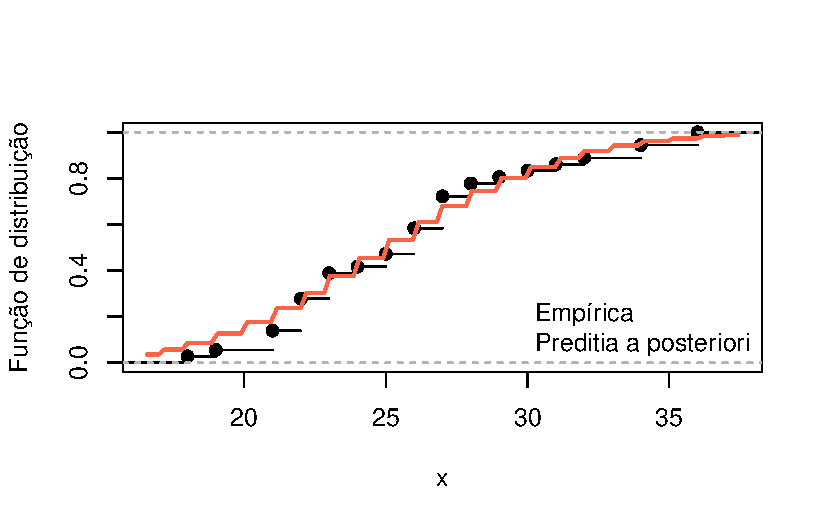
\includegraphics{poisson_files/figure-pdf/unnamed-chunk-3-1.pdf}

\section{O modelo Poisson para
taxas}\label{o-modelo-poisson-para-taxas-1}

A taxa é o cociente entre o número de casos de um evento em determinado
intervalo de tempo e a população em risco, definida em um espaço e no
mesmo intervalo de tempo ``pessoas-tempo''. Note que, pela definição, a
taxa é uma estatística.

Seja \(N\) o tamanho da população no espaço/tempo e seja \(y\) o número
de casos do evento de interesse. Então,

\[\hbox{taxa} = \frac{y}{N}\]

Contudo, como \(N\) tende a ser muito maior que \(y\), é comum reportar
a taxa vezes \(10^k\), para algum \(k>0\).

Exemplo: Segundo o Anuário de Segurança Pública 2022, em 2021 houveram
68.885 casos de estupro. Considerando uma população de 212,7 milhões de
habitantes, a taxa de estupro para aquele ano foi de
\[\frac{68.885}{212.700.000}=3,23\times 10^{-4}\] casos por pessoa-ano.

Multiplicando a taxa por \(10^5\), temos uma taxa de 32,3 casos para
cada 100.000 habitantes.

Agora,considere que \(\lambda\) é o parâmetro taxa (ou seja, caso por
\(10^k\) pessoas). Então,

\[\hat{\lambda}=\frac{y}{N}\] é a estimativa para \(\lambda\). Como
\(y\) é uma contagem, é razoável supor que
\[\lambda =\frac{1}{N}E(Y|\lambda),\] e um modelo com essa
parametrização seria \(y|\lambda\sim\hbox{Poisson}(\lambda n)\).

Agora, considere que a população está particionada em \(m\) localidades.
Para um dado intervalo de tempo, sejam \(N_i\) e \(y_i\) a população da
localidade \(i\) e seu respectivo número de casos observados. Suponha
ainda que a taxa \(\lambda\) é comum para a população e que \(y_i\) e
\(y_j\) são independentes dado \(\lambda\). Assumindo a distribuição
Poisson, teremos

\[L(\lambda)=\prod_{i=1}^m\frac{e^{-\lambda n_i}(\lambda N_i)^{y_i}}{y_i!}\varpropto \lambda^{\sum_{i=1}^m y_i}e^{-\lambda \sum_{i=1}^m N_i}=\lambda^{\sum_{i=1}^n y_i}e^{-\lambda N},\]
onde \(N=\sum_{i=1}^m N_i\) é o tamanho da população. Como a
verossimilhança pertence à família exponencial, temos que o modelo
Gama\((r,s)\) é conjugado gerando a posteriori

\[\lambda|\mathbf{y}\sim\hbox{Gama}\left(\sum_{i=1}^{m}y_i+r,N+s\right)\equiv \hbox{Gamma}(r_1,s_1).\]

Considere agora um novo valor observado da localidade \(i\). Sua
preditiva a posteriori é dada por

\[\begin{align}
f(y^*_i|\boldsymbol{y})&=\int_0^\infty f(y^*_i|\lambda)f(\lambda|\boldsymbol{y})d\lambda\\
&\int_0^\infty \frac{e^{-\lambda N_i}(\lambda N_i)^{y_i^*}}{y_i^*!}\frac{s_1^{r_1}}{\Gamma(r_1)}\lambda^{r_1-1}e^{-\lambda s_1}d\lambda\\
&=\frac{\Gamma(r_1+y_i^*)}{y_i^*!\Gamma(r_1)}\left(\frac{s_i}{N_i+s_i}\right)^{r_1}\left(1-\frac{s_i}{N_i+s_i}\right)^{y_i^*},
\end{align}\] ou seja,
\[y_i^*|\boldsymbol{y}\sim\text{Binomial Negativa}\left(r_1,\frac{s_1}{N_i+s_1}\right),\]
cujo valor esperado é \[E(y_i^*|\boldsymbol{y})=\frac{r_1}{s_1}N_i.\]
Observe que \(y_1^*\) e \(y_j^*\) possuem a mesma distribuição somente
se \(N_i=N_j\).

\phantomsection\label{exm}
\begin{longtable}[]{@{}ll@{}}
\toprule\noalign{}
Unidade Federativa & População Estimada (1º de Julho de 2024) \\
\midrule\noalign{}
\endhead
\bottomrule\noalign{}
\endlastfoot
São Paulo & 45.973.194 \\
Minas Gerais & 21.322.691 \\
Rio de Janeiro & 17.219.679 \\
Bahia & 14.850.513 \\
Paraná & 11.824.665 \\
Rio Grande do Sul & 11.229.915 \\
Pernambuco & 9.539.029 \\
Ceará & 9.233.656 \\
Pará & 8.664.306 \\
Santa Catarina & 8.058.441 \\
Goiás & 7.350.483 \\
Maranhão & 7.010.960 \\
Amazonas & 4.281.209 \\
Paraíba & 4.145.040 \\
Espírito Santo & 4.102.129 \\
Mato Grosso & 3.836.399 \\
Rio Grande do Norte & 3.446.071 \\
Piauí & 3.375.646 \\
Alagoas & 3.220.104 \\
Distrito Federal & \\
Mato Grosso do Sul & 2.901.895 \\
Sergipe & 2.291.077 \\
Rondônia & 1.746.227 \\
Tocantins & 1.577.342 \\
Acre & 880.631 \\
Amapá & 802.837 \\
Roraima & 716.793 \\
\end{longtable}

\phantomsection\label{exm}
\textbf{Crime de estupro de vulnerável no interior do Amazonas}

Os dados a seguir foram cedidos pelo Observatório de Violência de Gênero
no Amazonas e compreendem os anos entre 2010 e 2012. A população em
risco é o número de mulheres co menos de 14 anos.

\begin{longtable}[]{@{}lll@{}}
\toprule\noalign{}
Cidade & Vítimas & Populacao feminina \\
\midrule\noalign{}
\endhead
\bottomrule\noalign{}
\endlastfoot
Amatura & 3 & 639 \\
Atalaia do Norte & 6 & 905 \\
Barreirinha & 12 & 1899 \\
Benjamin Constant & 2 & 2036 \\
Boa Vista do Ramos & 6 & 1060 \\
Fonte Boa & 0 & 1438 \\
Jutai & 1 & 1143 \\
Maues & 13 & 3421 \\
Nhamunda & 9 & 1168 \\
Parintins & 20 & 6700 \\
Santo Antonio do Ica & 7 & 1608 \\
Sao Paulo de Olivenca & 5 & 2033 \\
Tabatinga & 8 & 3095 \\
Tonantins & 1 & 1186 \\
\end{longtable}

Abaixo, organizamos os dados. A população é dividida por \(10^5\) para
que a taxa seja interpretada como número de casos para cada 100.000
mulheres menores de 14 anos.

\begin{Shaded}
\begin{Highlighting}[]
\CommentTok{\# banco de dados}
\NormalTok{casos }\OtherTok{\textless{}{-}} \FunctionTok{c}\NormalTok{( }\DecValTok{3}\NormalTok{, }\DecValTok{6}\NormalTok{, }\DecValTok{12}\NormalTok{, }\DecValTok{2}\NormalTok{, }\DecValTok{6}\NormalTok{, }\DecValTok{0}\NormalTok{, }\DecValTok{1}\NormalTok{, }\DecValTok{13}\NormalTok{, }\DecValTok{9}\NormalTok{, }\DecValTok{20}\NormalTok{, }\DecValTok{7}\NormalTok{, }\DecValTok{5}\NormalTok{, }\DecValTok{8}\NormalTok{, }\DecValTok{1}\NormalTok{ )   }

\NormalTok{pop }\OtherTok{\textless{}{-}} \FunctionTok{c}\NormalTok{(}\DecValTok{639}\NormalTok{, }\DecValTok{905}\NormalTok{, }\DecValTok{1899}\NormalTok{, }\DecValTok{2036}\NormalTok{, }\DecValTok{1060}\NormalTok{, }\DecValTok{1438}\NormalTok{, }\DecValTok{1143}\NormalTok{, }\DecValTok{3421}\NormalTok{, }\DecValTok{1168}\NormalTok{, }\DecValTok{6700}\NormalTok{, }\DecValTok{1608}\NormalTok{, }\DecValTok{2033}\NormalTok{, }\DecValTok{3095}\NormalTok{, }\DecValTok{1186}\NormalTok{)}
\NormalTok{pop }\OtherTok{\textless{}{-}}\NormalTok{ pop}\SpecialCharTok{/}\DecValTok{10}\SpecialCharTok{\^{}}\DecValTok{5}

\NormalTok{municipios }\OtherTok{\textless{}{-}} \FunctionTok{c}\NormalTok{( }\StringTok{\textquotesingle{}Amaturá\textquotesingle{}}\NormalTok{, }\StringTok{\textquotesingle{}Ataláia do Norte\textquotesingle{}}\NormalTok{, }\StringTok{\textquotesingle{}Barreirinha\textquotesingle{}}\NormalTok{, }\StringTok{\textquotesingle{}Benjamin Constant\textquotesingle{}}\NormalTok{,}\StringTok{\textquotesingle{}Boa Vista do Ramos\textquotesingle{}}\NormalTok{, }\StringTok{\textquotesingle{}Fonte Boa\textquotesingle{}}\NormalTok{, }\StringTok{\textquotesingle{}Jutaí\textquotesingle{}}\NormalTok{, }\StringTok{\textquotesingle{}Maués\textquotesingle{}}\NormalTok{, }\StringTok{\textquotesingle{}Nhamunda\textquotesingle{}}\NormalTok{, }\StringTok{\textquotesingle{}Parintins\textquotesingle{}}\NormalTok{, }\StringTok{\textquotesingle{}Sto Antônio do Iça\textquotesingle{}}\NormalTok{, }\StringTok{\textquotesingle{}São Paulo de Olivença\textquotesingle{}}\NormalTok{, }\StringTok{\textquotesingle{}Tabatinga\textquotesingle{}}\NormalTok{,}\StringTok{\textquotesingle{}Tonantins\textquotesingle{}}\NormalTok{)}
\end{Highlighting}
\end{Shaded}

A veromissilhança é dada por
\[L(\lambda)\propto \lambda^{93}e^{-0,28331\lambda }.\] Utilizando a
priori \(\lambda\sim\hbox{Gama}(.5,.00001)\), teremos a posteriori
\(\lambda\sim\hbox{Gama}(93.5,0.28332)\)

Vamos calcular o número de casos esperado segundo a preditiva a
posteriori para cada município.

\begin{Shaded}
\begin{Highlighting}[]
\NormalTok{r }\OtherTok{\textless{}{-}}\NormalTok{ .}\DecValTok{5}
\NormalTok{s }\OtherTok{\textless{}{-}}\NormalTok{ .}\DecValTok{00001}

\NormalTok{r1 }\OtherTok{\textless{}{-}} \FunctionTok{sum}\NormalTok{(casos) }\SpecialCharTok{+}\NormalTok{ r}
\NormalTok{s1 }\OtherTok{\textless{}{-}} \FunctionTok{sum}\NormalTok{(pop) }\SpecialCharTok{+}\NormalTok{ s}

\NormalTok{esperado }\OtherTok{\textless{}{-}}\NormalTok{ r1 }\SpecialCharTok{*}\NormalTok{ pop }\SpecialCharTok{/}\NormalTok{ s1}
\end{Highlighting}
\end{Shaded}

O gráfico abaixo apresenta o valor da média da preditiva a posteriori
contra o número de casos observados. Como esperado, os pares ordenados
flutuam em torno da linha \(y=x\).

\begin{Shaded}
\begin{Highlighting}[]
\FunctionTok{plot}\NormalTok{(casos, esperado, }\AttributeTok{xlab =} \StringTok{\textquotesingle{}Casos observados\textquotesingle{}}\NormalTok{, }\AttributeTok{ylab =} \StringTok{\textquotesingle{}Casos esperados\textquotesingle{}}\NormalTok{)}
\FunctionTok{abline}\NormalTok{(}\DecValTok{0}\NormalTok{,}\DecValTok{1}\NormalTok{,}\AttributeTok{lty =} \DecValTok{2}\NormalTok{)}
\end{Highlighting}
\end{Shaded}

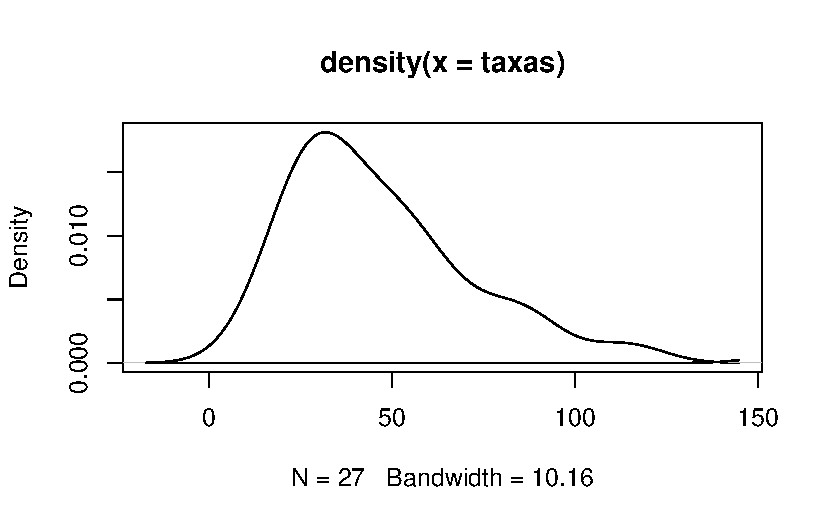
\includegraphics{poisson_files/figure-pdf/unnamed-chunk-6-1.pdf}

Mesmo que os pontos no gráfico acima estejam flutuando em torno da reta
\(y=x\), é importante determinar se sua distância até a reta é razoável.
Podemos construir intervalos de 95\% (de predição) para \(y^*_i\)
utilizando os quantis da preditiva a posteriori, ou seja, encontrando
\(q_1\) e \(q_2\) tais que \[\begin{align}
P(Y_i^*\leq q_1|\boldsymbol{y})&=0,025\\
P(Y_i^*\leq q_2|\boldsymbol{y})&=0,975.
\end{align}
\]

Observe ainda que
\[0,95\approx P(q_1\leq Y_i^*\leq q_2|\boldsymbol{y})=P\left(\frac{q_1}{N_i}\leq \frac{Y_i^*}{N_i}\leq \frac{q_2}{N_i}|\boldsymbol{y}\right),\]
o que implica que \((q_1,q_2)/N_i\) é um intervalo para taxa esperada.
Abaixo construímos os intervalos de 95\% (de predição) e colocamos o
número de casos observados.

\begin{Shaded}
\begin{Highlighting}[]
\CommentTok{\# limites do intervalo}
\NormalTok{lim\_inf }\OtherTok{\textless{}{-}} \FunctionTok{qnbinom}\NormalTok{(.}\DecValTok{025}\NormalTok{, }\AttributeTok{size =}\NormalTok{ r1, }\AttributeTok{prob =}\NormalTok{ s1}\SpecialCharTok{/}\NormalTok{(pop}\SpecialCharTok{+}\NormalTok{s1))}

\NormalTok{lim\_sup }\OtherTok{\textless{}{-}} \FunctionTok{qnbinom}\NormalTok{(.}\DecValTok{975}\NormalTok{, }\AttributeTok{size =}\NormalTok{ r1, }\AttributeTok{prob =}\NormalTok{ s1}\SpecialCharTok{/}\NormalTok{(pop}\SpecialCharTok{+}\NormalTok{s1))}

\CommentTok{\# gráfico}
\FunctionTok{plot.new}\NormalTok{()}
\FunctionTok{plot.window}\NormalTok{( }\AttributeTok{xlim =} \FunctionTok{c}\NormalTok{(}\SpecialCharTok{{-}}\DecValTok{500}\NormalTok{,}\DecValTok{1000}\NormalTok{), }\AttributeTok{ylim=}\FunctionTok{c}\NormalTok{(}\DecValTok{0}\NormalTok{,}\DecValTok{15}\NormalTok{))}
\FunctionTok{segments}\NormalTok{(lim\_inf}\SpecialCharTok{/}\NormalTok{pop,}\DecValTok{1}\SpecialCharTok{:}\DecValTok{14}\NormalTok{,lim\_sup}\SpecialCharTok{/}\NormalTok{pop,}\DecValTok{1}\SpecialCharTok{:}\DecValTok{14}\NormalTok{, }\AttributeTok{lwd =} \DecValTok{2}\NormalTok{)}
\FunctionTok{text}\NormalTok{(}\SpecialCharTok{{-}}\DecValTok{500}\NormalTok{,}\DecValTok{1}\SpecialCharTok{:}\DecValTok{14}\NormalTok{, municipios, }\AttributeTok{adj =}\DecValTok{0}\NormalTok{ )}
\FunctionTok{points}\NormalTok{(casos}\SpecialCharTok{/}\NormalTok{pop, }\DecValTok{1}\SpecialCharTok{:}\DecValTok{14}\NormalTok{, }\AttributeTok{pch =} \DecValTok{22}\NormalTok{, }\AttributeTok{cex =}\NormalTok{.}\DecValTok{9}\NormalTok{, }\AttributeTok{bg =} \StringTok{\textquotesingle{}red\textquotesingle{}}\NormalTok{)}
\end{Highlighting}
\end{Shaded}

\includegraphics{poisson_files/figure-pdf/unnamed-chunk-7-1.pdf}

Alguns municípios, como Nanhunda, foram substimados, enquanto outros,
como Fonte Boa, foram superestimados. Para estes 14 intervalos, é
esperado que \(14\times 0,05=0,7\) deles não cubram \(y_i\), o que não
está ocorrendo. Portanto, considerar que todos os municípios possuem a
mesma taxa pode ser um equívoco.

\section{Exercícios}\label{exercuxedcios-3}

\subsection{Mortes por coice de
cavalo}\label{mortes-por-coice-de-cavalo-1}

Ladislaus Bortkiewicz é o responsável pela popularização da distribuição
Poisson. Em seu livro intitulado A Lei dos Pequenos Números, é
apresentado um conjunto de dados no qual foi rastreado o número de
mortes por coice de cavalo em 14 corpos do exército prussiano ao longo
de 20 anos (de 1875 a 1894).

\begin{longtable}[]{@{}lllll@{}}
\toprule\noalign{}
Mortes por corpo \(\times\) ano & 0 & 1 & 2 & 3 \\
\midrule\noalign{}
\endhead
\bottomrule\noalign{}
\endlastfoot
109 & 65 & 22 & 3 & 1 \\
\end{longtable}

Determine se a distribuição Poisson é adequada para este conjunto de
dados. Em caso afirmativo, estime a taxa e dê um intervalo de
credibilidade de 95\%.

\subsection{Suicídios no Amazonas considerando capital e
interior}\label{suicuxeddios-no-amazonas-considerando-capital-e-interior-1}

O Amazonas possui uma característica peculiar: aproximadamente 50\% da
população vive na capital. Vimos anteriormente que o número de
suicídios, considerando os anos entre 2021 e 2023, podem ser modelados
por uma Poisson. A tabela abaixo divide esses dados entre capital e
interior.

\begin{longtable}[]{@{}lllll@{}}
\caption{Número de suicídios divididos entre capital e
interior}\tabularnewline
\toprule\noalign{}
Ano & 2021 & 2022 & 2023 & Total \\
\midrule\noalign{}
\endfirsthead
\toprule\noalign{}
Ano & 2021 & 2022 & 2023 & Total \\
\midrule\noalign{}
\endhead
\bottomrule\noalign{}
\endlastfoot
Capital & 133 & 124 & 138 & 395 \\
Interior & 164 & 173 & 201 & 538 \\
\end{longtable}

Determine se há evidências de que essas taxas são diferentes.

\bookmarksetup{startatroot}

\chapter*{References}\label{references}
\addcontentsline{toc}{chapter}{References}

\markboth{References}{References}

\phantomsection\label{refs}
\begin{CSLReferences}{1}{0}
\bibitem[\citeproctext]{ref-polack2020safety}
Polack, Fernando P, Stephen J Thomas, Nicholas Kitchin, Judith Absalon,
Alejandra Gurtman, Stephen Lockhart, John L Perez, et al. 2020.
{``Safety and Efficacy of the BNT162b2 mRNA Covid-19 Vaccine.''}
\emph{New England Journal of Medicine} 383 (27): 2603--15.

\end{CSLReferences}




\end{document}
